\documentclass[10pt]{article}
\usepackage[vietnamese]{babel}
\usepackage[utf8]{inputenc}
\usepackage[T5]{fontenc}
\usepackage{amsmath}
\usepackage{amsfonts}
\usepackage{amssymb}
\usepackage[version=4]{mhchem}
\usepackage{stmaryrd}
\usepackage{graphicx}
\usepackage[export]{adjustbox}
\graphicspath{ {./images/} }
\usepackage{caption}
\usepackage{multirow}

\def\AA{\mathring{\mathrm{A}}}

\begin{document}
\captionsetup{singlelinecheck=false}
1.5. Hiện tượng nào sau đây là hiện tượng vật lí, hiện tượng nào là hiện tượng hoá học?\\
a) Vào mùa hè, băng ở hai cực Trái Đất tan dần.\\
b) Thổi hơi thở của chúng ta vào nước vôi trong làm nước vôi trong vẩn đục.\\
c) Đốt cháy đường mía tạo thành chất màu đen và có mùi khét.\\
d) Sắt bị nam châm hút ra khỏi hỗn hợp gồm bột sắt (iron) và lưu huỳnh (sulfur).\\
e) Đun nóng hỗn hợp gồm sắt và lưu huỳnh trong ống nghiệm. Hỗn hợp nóng sáng lên và chuyển dần thành chất rắn màu đen.\\
1.6. Hãy phân tích và chỉ ra ở giai đoạn nào diễn ra quá trình biến đổi vật lí, giai đoạn nào diễn ra quá trình biến đổi hoá học trong các hiện tượng sau: "Khi sản xuất vôi sông, người ta đập đá vôi thành những cục nhỏ có kích thước thích hợp cho vào lò nung, nung đá vôi ta được vôi sống và khí carbonic. Khuấy vôi sống với ît nước ta được nước vôi đặc, thêm nước vào nước vôi đặc ta được nước vôi loãng."\\
1.7. Thanh sắt được nung nóng, dát mỏng, kéo dài thành dây sắt. Sau đó tiếp tục nung nóng dây sắt thi thu được chất bột màu nâu. Hãy chỉ ra đâu là hiện tượng vật lí, đâu là hiện tượng hoá học.\\
1.8. Hãy lập sơ đồ tư duy để hệ thống hoá kiến thức "Bài 1. Nhập môn hoá học" trong SGK.

\section*{Dữ kiện sử dụng cho bài tập 1.9 và 1.10.}
Để nghiên cứu thành phần hoá học, hoạt tính kháng oxi hoá và hoạt tính kháng khuẩn của tinh dầu vỏ chanh, các nhà nghiên cứu đã thực hiện các công việc sau:

\begin{itemize}
  \item Tìm hiểu về cây chanh, công dụng và tác dụng dược lí của chanh cũng như hoạt tính kháng oxi hoá, kháng vi sinh vật của nó thông qua các công bố khoa học trong và ngoài nước.
  \item Thu hái mẫu vỏ chanh tại vườn chanh.
  \item Khảo sát sự trích li tinh dầu bằng phương pháp chưng cất lôi cuốn hơi nước.
  \item Thử hoạt tính kháng oxi hoá, thử hoạt tính kháng vi sinh vật.\\
1.9. Hãy cho biết trong nghiên cứu trên, các nhà nghiên cứu đã sử dụng phương pháp nghiên cứu nào? Hãy chỉ phương pháp sử dụng cho mỗi công việc trên.\\
1.10. Hãy chỉ rõ các bước nghiên cứu trong nghiên cứu trên tương ứng với những bước nào trong phương pháp nghiên cứu hoá học.
\end{itemize}

\section*{Chương 1. CẤU TẬO NGUYÊN TỬ}
\section*{2 THÀNH PHẦN CỦA NGUYÊN TỬ}
2.1. Phát biểu nào dưới đây không đúng?\\
A. Nguyên tử được cấu thành từ các hạt cơ bản là proton, neutron và electron.\\
B. Hầu hết hạt nhân nguyên tử được cấu thành từ các hạt proton và neutron.\\
C. Vỏ nguyên tử được cấu thành bởi các hạt electron.\\
D. Nguyên tử có cấu trúc đặc khít, gồm vỏ nguyên tử và hạt nhân nguyên tử.\\
2.2. Cho 1 mol kim loại X . Phát biểu nào dưới đây đúng?\\
A. $1 \mathrm{~mol} X$ chứa số lượng nguyên tử bằng số lượng nguyên tử trong 1 mol nguyên tử hydrogen.\\
B. $1 \mathrm{~mol} X$ chứa số lượng nguyên tử bằng số lượng nguyên tử trong $\frac{1}{12} \mathrm{~mol}$ carbon.\\
C. 1 mol X có khối lượng bằng khối lượng 1 mol hydrogen.\\
D. $1 \mathrm{~mol} X$ có khối lượng bằng $\frac{1}{2}$ khối lượng 1 mol carbon.\\
2.3. Thành phần nào không bị lệch hướng trong trường điện?\\
A. Tia $\alpha$.\\
B. Proton.\\
C. Nguyên tử hydrogen.\\
D. Tia âm cực.\\
2.4. Phát biểu nào sai khi nói về neutron?\\
A. Tồn tại trong hạt nhân nguyên tử.\\
B. Có khối lượng bằng khối lượng proton.\\
C. Có khối lượng lớn hơn khối lượng electron.\\
D. Không mang điện.\\
2.5. Nguyên tử $R$ có điện tích lớp vỏ nguyên tử là $-41,6 \cdot 10^{-19} \mathrm{C}$. Điều khẳng định nào sau đây là không chính xác?\\
A. Lớp vỏ nguyên tử $R$ có 26 electron.\\
B. Hạt nhân nguyên tử $R$ có 26 proton.\\
C. Hạt nhân nguyên tử $R$ có 26 neutron.\\
D. Nguyên tử $R$ trung hoà về điện.\\
2.6. Hạt nhân của nguyên tử nguyên tố A có 24 hạt, trong đó số hạt không mang điện là 12. Số electron trong A là\\
A. 12 .\\
B. 24.\\
C. 13.\\
D. 6 .\\
2.7. Trong nguyên tử Al , số hạt mang điện tích dương là 13 , số hạt không mang điện là 14. Số hạt electron trong Al là bao nhiêu?\\
A. 13 .\\
B. 15.\\
C. 27 .\\
D. 14 .\\
2.8. Đặc điểm của electron là\\
A. mang điện tích dương và có khối lượng.\\
B. mang điện tích âm và có khối lượng.\\
C. không mang điện và có khối lượng.\\
D. mang điện tích âm và không có khối lượng.\\
2.9. Nhận định nào sau đây không đúng?\\
A. Tất cả các hạt nhân nguyên tử đều chứa proton và neutron.\\
B. Nguyên tử có kích thước vô cùng nhỏ và trung hoà về điện.\\
C. Lớp vỏ nguyên tử chứa electron mang điện tích âm.\\
D. Khối lượng nguyên tử hầu hết tập trung ở hạt nhân.\\
2.10. Cho các phát biểu sau:\\
(1) Tất cả các hạt nhân nguyên tử đều đươc cấu tạo từ các hạt proton và neutron.\\
(2) Khối lượng nguyên tử tập trung phần lớn ở lớp vỏ.\\
(3) Trong nguyên tử, số electron bằng số proton.\\
(4) Trong hạt nhân nguyên tử, hạt mang điện là proton và electron.\\
(5) Trong nguyên tử, hạt electron có khối lượng không đáng kể so với các hạt còn lại.\\
Số phát biểu đúng là\\
A. 1 .\\
B. 2 .\\
C. 3.\\
D. 4.\\
2.11. Kết quả nào trong thí nghiệm bắn phá lá vàng của Rutherford chỉ ra sự tồn tại của hạt nhân nguyên tử?\\
2.12. Hãy điền những dữ liệu còn thiếu vào các chỗ trống trong các câu sau:\\
a) Trong ống tia âm cực, tia âm cực được phát ra từ điện cực âm được gọi là (1)\\
b) Đơn vị nhỏ nhất của một nguyên tố có thể tồn tại đơn lẻ hoặc tồn tại trong các phân tử được gọi là (2).\\
c) Hạt mang điện tích dương được tìm thấy trong hạt nhân nguyên tử được gọi là (3)...\\
d) Hạt không mang điện tồn tại trong hạt nhân nguyên tử được gọi là (4) $\_\_\_\_$\\
e) Hạt trong nguyên tử có khối lượng nhỏ nhất và khối lượng lớn nhất, tương ứng là (5) $\_\_\_\_$ và (6). $\_\_\_\_$\\
2.13. Tia âm cực phát ra trong ống âm cực bị lệch hướng khi đặt trong trường từ. Một dây dẫn mang điện cũng có thể bị hút bởi trường từ. Tia âm cực bị lệch hướng khi đặt gần một vật mang điện âm. Tính chất nào của tia âm cực được thể hiện qua các hiện tượng này?\\
2.14. Electron sinh ra trong ống tia âm cực chứa khí neon có khác electron sinh ra trong ống tia âm cực chứa khí chlorine không? Vì sao?\\
2.15. Nguyên tử mang điện tích dương, điện tích âm hay trung hoà? Giải thích vì sao một nguyên tử có thể tồn tại ở trạng thái này.\\
2.16. $X$ là nguyên tố hoá học có trong thành phần của chất có tác dụng oxi hoá và sát khuẩn cực mạnh, thường được sử dụng với mục đích khử trùng và tẩy trắng trong lĩnh vực thuỷ sản, dệt nhuộm, xử lí nước cấp, nước thải, nước bể bơi. Nguyên tử $X$ có tổng số các loại hạt bằng 52 , trong đó số hạt mang điện nhiều hơn số hạt không mang điện là 16 hạt. Xác định thành phần cấu tạo của nguyên tử $X$.\\
2.17. Các hợp chất của nguyên tố $Y$ được sử dụng như là vật liệu chịu lửa trong các lò sản xuất sắt, thép, kim loại màu, thuỷ tinh và xi măng. Oxide của $Y$ và các hợp chất khác cũng được sử dụng trong nông nghiệp, công nghiệp hoá chất và xây dựng. Nguyên tử Y có tổng số các hạt là 36. Số hạt không mang điện bằng một nửa hiệu số giữa tổng số hạt với số hạt mang điện tích âm. Xác định thành phần cấu tạo của nguyên tử Y.\\
2.18. Nitrogen giúp bảo quản tinh trùng, phôi, máu và tế bào gốc. Biết nguyên tử nitrogen có tổng số hạt là 21 . Số hạt không mang điện chiếm $33,33 \%$. Xác định số đơn vị điện tích hạt nhân của nitrogen.\\
2.19. Magnesium oxide ( MgO ) được sử dụng để làm dịu cơn đau ợ nóng và chua của chứng đau dạ dày. Tổng số hạt mang điện trong hợp chất MgO là 40 . Số hạt mang điện trong nguyên tử Mg nhiều hơn số hạt mang điện trong nguyên tử O là 8 . Xác định điện tích hạt nhân của Mg và O .\\
2.20. Helium là một khí hiếm được sử dụng rộng rãi trong nhiều ngành công nghiệp như hàng không, hàng không vũ trụ, điện tử, điện hạt nhân và chăm sóc sức khoẻ. Nguyên tử helium có 2 proton, 2 neutron và 2 electron. Cho biết khối lượng của electron trong nguyên tử helium chiếm bao nhiêu phần trăm khối lượng nguyên tử.\\
2.21*. Khi phóng chùm tia $\alpha$ vào một lá vàng mỏng, người ta thấy rằng trong khoảng $10^{8}$ hạt $\alpha$ có một hạt gặp hạt nhân.\\
a) Một cách gần đúng, hãy xác định đường kính của hạt nhân so với đường kính của nguyên tử.\\
b) Với sự thừa nhận kết quả trên, hãy tính đường kính của nguyên tử nếu ta coi hạt nhân có kích thước như một quả bóng bàn có đường kính bằng 3 cm .\\
2.22*. Calcium là một loại khoáng chất có vai trò rất quan trọng trong cơ thể người. Trong cơ thể, calcium chiếm 1,5-2\% trọng lượng, 99\% lượng calcium tồn tại trong xương, răng, móng và $1 \%$ trong máu. Calcium kết hợp với phosphorus là thành phần cấu tạo cơ bản của xương và răng, làm cho xương và răng chắc khoẻ. Khối lượng riêng của calcium kim loại là $1,55 \mathrm{~g} / \mathrm{cm}^{3}$. Giả thiết rằng, trong tinh thể calcium, các nguyên tử là những hình cầu chiếm $74 \%$ thể tích tinh thể, phần còn lại là khe rỗng. Xác định bán kính nguyên tử calcium. Cho nguyên tử khối của calcium là 40 .\\
Cho biết công thức tính thể tích hình cầu là $V=\frac{4 \pi r^{3}}{3}$, trong đó $r$ là bán kính hình cầu.\\
2.23*. Bán kính nguyên tử và khối lượng mol nguyên tử iron lần lượt là 1,28 Å và $56 \mathrm{~g} / \mathrm{mol}$. Tính khối lượng riêng của iron. Biết rằng trong tinh thể, các tinh thể iron chiếm $74 \%$ thể tích còn lại là phần rổng.\\
2.24*. Nguyên tử Fe ở $20^{\circ} \mathrm{C}$ có khối lượng riêng là $7,87 \mathrm{~g} / \mathrm{cm}^{3}$. Với giả thiết này, tinh thể nguyên tử Fe là những hình cầu chiếm $75 \%$ thể tích tinh thể, phần còn lại là những khe rỗng giữa các quả cầu. Cho biết khối lượng nguyên tử của Fe là 55,847 . Tính bán kính nguyên tử gần đúng của Fe .\\
$2.25^{*}$. Nguyên tử kẽm $(\mathrm{Zn})$ có nguyên tử khối bằng 65 u. Thực tế hầu như toàn bộ khối lượng nguyên tử tập trung ở hạt nhân, với bán kính $\mathrm{r}=2 \times 10^{-15} \mathrm{~m}$. Khối lượng riêng của hạt nhân nguyên tử kẽm là bao nhiêu tấn trên một centimet khối (tấn/ $\mathrm{cm}^{3}$ )?

\section*{3 NGUYÊN TỐ HOÁ HỌC}
3.1. Cho các phát biểu sau:\\
(1) Trong một nguyên tử luôn có số proton bằng số electron và bằng số đơn vị điện tích hạt nhân.\\
(2) Tổng số proton và số electron trong một hạt nhân được gọi là số khối.\\
(3) Số khối là khối lượng tuyệt đối của nguyên tử.\\
(4) Số proton bằng số đơn vị điện tích hạt nhân.\\
(5) Đồng vị là các nguyên tố có cùng số proton nhưng khác nhau về số neutron.

Số phát biểu không đúng là\\
A. 1 .\\
B. 2 .\\
C. 3.\\
D. 4 .\\
3.2. Cho các phát biểu sau, phát biểu nào đúng về đồng vị?\\
A. Những phân tử có cùng số hạt proton nhưng khác nhau về số hạt neutron là đồng vị của nhau.\\
B. Những ion có cùng số hạt proton nhưng khác nhau về số hạt electron là đồng vị của nhau.\\
C. Những chất có cùng số hạt proton nhưng khác nhau về số hạt neutron là đồng vị của nhau.\\
D. Những nguyên tử có cùng số hạt proton nhưng khác nhau về số hạt neutron là đồng vị của nhau.\\
3.3. Có những phát biểu sau đây về các đồng vị của một nguyên tố hoá học:\\
(1) Các đồng vị có tính chất hoá học giống nhau.\\
(2) Các đồng vị có tính chất vật lí khác nhau.\\
(3) Các đồng vị có cùng số electron ở vỏ nguyên tử.\\
(4) Các đồng vị có cùng số proton nhưng khác nhau về số khối.

Trong các phát biểu trên, số phát biểu đúng là\\
A. 1 .\\
B. 2 .\\
C. 3 .\\
D. 4 .\\
3.4. Nguyên tử của nguyên tố $A$ có 56 electron, trong hạt nhân có 81 neutron. Kí hiệu của nguyên tử nguyên tố $A$ là\\
A. ${ }_{56}^{137} \mathrm{~A}$.\\
B. ${ }_{137}^{56} \mathrm{~A}$.\\
C. ${ }_{56}^{81} \mathrm{~A}$.\\
D. ${ }_{81}^{56} \mathrm{~A}$.\\
3.5. Trong tự nhiên, oxygen có 3 đồng vị là ${ }^{16} \mathrm{O},{ }^{17} \mathrm{O},{ }^{18} \mathrm{O}$. Có bao nhiêu loại phân tử $\mathrm{O}_{2}$ ?\\
A. 3 .\\
B. 6.\\
C. 9.\\
D. 12 .\\
3.6. Có 3 nguyên tử: ${ }_{6}^{12} X,{ }_{7}^{14} Y,{ }_{6}^{14} Z$. Những nguyên tử nào là đồng vị của một nguyên tố?\\
A. $X, Y$.\\
B. $Y, Z$.\\
C. $X, Z$.\\
D. $X, Y, Z$.\\
3.7. Boron có trong một số loại trái cây, thực phẩm mà chúng ta nạp vào cơ thể hằng ngày. Chúng có tác dụng rất tốt cho việc cải thiện một số chức năng của não bộ và cấu trúc, mật độ của xương. Nguyên tử boron có khối lượng nguyên tử là 10,81 amu. Tuy nhiên, không có nguyên tử boron nào có khối lượng chính xác là 10,81 amu. Hãy giải thích điều đó.\\
3.8. Hoàn thành các thông tin trong bảng sau:

\begin{center}
\begin{tabular}{|l|l|l|l|l|l|l|}
\hline
Nguyên tố & Kí hiệu & Số hiệu nguyên tử & Số khối & Số proton & Số neutron & Số electron \\
\hline
Sodium & Na & 11 & 22 & ? & ? & ? \\
\hline
Fluorine & F & 9 & 19 & ? & ? & ? \\
\hline
Bromine & Br & ? & 80 & ? & 45 & ? \\
\hline
Calcium & Ca & ? & 40 & 20 & ? & ? \\
\hline
Hydrogen & H & ? & 1 & ? & ? & 1 \\
\hline
Radon & Rn & 86 & ? & ? & 136 & ? \\
\hline
\end{tabular}
\end{center}

3.9. Một nguyên tố X tồn tại dưới dạng ba đồng vị tự nhiên có thông tin được cho trong bảng dưới đây:

\begin{center}
\begin{tabular}{|l|l|l|}
\hline
Đồng vị & \% số nguyên tử trong tự nhiên & Số khối \\
\hline
1 & 90,51 & 20 \\
\hline
2 & 0,27 & 21 \\
\hline
3 & 9,22 & 22 \\
\hline
\end{tabular}
\end{center}

Tính nguyên tử khối trung bình của nguyên tố $X$.\\
3.10. Hoàn thành những thông tin còn thiếu trong bảng sau:

\begin{center}
\begin{tabular}{|l|l|l|l|}
\hline
Nguyên tử & Kí hiệu nguyên tử & Số hiệu nguyên tử & Số khối \\
\hline
Europium & \( { }_{63}^{151} \mathrm{Eu} \) & ? & ? \\
\hline
Silver & ? & 47 & 109 \\
\hline
Tellurium & \( { }_{52}^{?} \mathrm{Te} \) & ? & 128 \\
\hline
\end{tabular}
\end{center}

3.11. Cho biết số proton, neutron và electron của nguyên tử ${ }_{30}^{65} \mathrm{Zn}$.\\
3.12. Nguyên tử Mg có ba đồng vị ứng với thành phần phần trăm về số nguyên tử như sau:

\begin{center}
\begin{tabular}{|c|c|c|c|}
\hline
Đồng vị & ${ }^{24} \mathbf{M g}$ & ${ }^{25} \mathbf{M g}$ & ${ }^{26} \mathbf{M g}$ \\
\hline
$\%$ & 78,6 & 10,1 & 11,3 \\
\hline
\end{tabular}
\end{center}

Giả sử trong hỗn hợp nói trên có 50 nguyên tử ${ }^{25} \mathrm{Mg}$, số nguyên tử tương ứng của hai đồng vị ${ }^{24} \mathrm{Mg}$ và ${ }^{26} \mathrm{Mg}$ lần lượt là:\\
A. 389 và 56 .\\
B. 56 và 389 .\\
C. 495 và 56 .\\
D. 56 và 495 .\\
3.13*. Hãy so sánh:\\
a) Số lượng hợp chất và số lượng nguyên tố.\\
b) Số lượng nguyên tố và số lượng đồng vị.

Giải thích.\\
3.14*. Oxide của kim loại $\mathrm{M}\left(\mathrm{M}_{2} \mathrm{O}\right)$ được ứng dụng rất nhiều trong ngành hoá chất như sản xuất xi măng, sản xuất phân bón, ... Trong sản xuất phân bón, chúng ta thường thấy $\mathrm{M}_{2} \mathrm{O}$ có màu trắng, tan nhiều trong nước và là thành phần không thể thiếu cho mọi loại cây trồng. Tổng số hạt cơ bản trong phân tử $X$ có công thức $\mathrm{M}_{2} \mathrm{O}$ là 140 , trong phân tử $X$ có tổng số hạt mang điện nhiều hơn số hạt không mang điện là 44. Xác định công thức phân tử của $\mathrm{M}_{2} \mathrm{O}$.\\
3.15*. Hợp chất $X Y_{2}$ phổ biến trong sử dụng để làm cơ chế đánh lửa bằng bánh xe trong các dạng súng cổ. Mỗi phân tử $X Y_{2}$ có tổng các hạt proton, neutron, electron bằng 178; trong đó, số hạt mang điện nhiều hơn số hạt không mang điện là 54, số hạt mang điện của $X$ ít hơn số hạt mang điện của $Y$ là 12. Hãy xác định kí hiệu hoá học của $\mathrm{X}, \mathrm{Y}$.

\section*{Bai \\
 4 \\
 CẤU TRÚC LỚP VỎ ELECTRON CỦA NGUYÊN TỬ}
4.1. Theo mô hình nguyên tử Rutherford - Bohr, vị trí nào trong số các vị trí $\mathrm{A}, \mathrm{B}$, $\mathrm{C}, \mathrm{D}$ trong hình sau mà electron không xuất hiện?\\
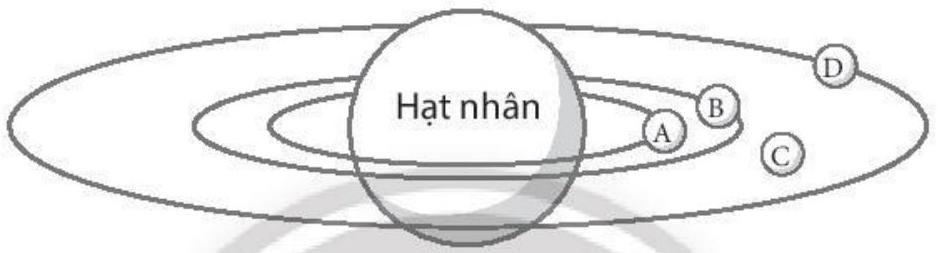
\includegraphics[max width=\textwidth, center]{2025_10_23_883c4b146e2332109fcdg-09}\\
A. Vị trí A.\\
B. Vị trí B.\\
C. Vị trí C.\\
D. Vị trí D.\\
4.2. Lớp electron thứ 3 có bao nhiêu phân lớp?\\
A. 1 .\\
B. 2 .\\
C. 3 .\\
D. 4 .\\
4.3. Phát biểu nào sao đây đúng?\\
A. Số phân lớp electron có trong lớp N là 4 .\\
B. Số phân lớp electron có trong lớp M là 4 .\\
C. Số orbital có trong lớp N là 9 .\\
D. Số orbital có trong lớp M là 8 .\\
4.4. Phát biểu nào sau đây đúng?\\
A. Lớp K là lớp xa hạt nhân nhất.\\
B. Các electron trong cùng một lớp có mức năng lượng bằng nhau.\\
C. Các electron trên cùng phân lớp có mức năng lượng bằng nhau.\\
D. Lớp N có 4 orbital.\\
4.5. Phát biểu nào đúng khi nói về các orbital trong một phân lớp electron?\\
A. Có cùng sự định hướng không gian.\\
B. Có cùng mức năng lượng.\\
C. Khác nhau về mức năng lượng.\\
D. Có hình dạng không phụ thuộc vào đặc điểm mỗi phân lớp.\\
4.6. Phát biểu nào sau đây không đúng?\\
A. Lớp $M$ có 9 phân lớp.\\
B. Lớp L có 4 orbital.\\
C. Phân lớp p có 3 orbital.\\
D. Năng lượng của electron trên lớp K là thấp nhất.\\
4.7. Cấu hình electron nào sau đây viết sai?\\
A. $1 s^{2} 2 s^{2} 2 p^{5}$.\\
B. $1 s^{2} 2 s^{2} 2 p^{6} 3 s^{2} 3 p^{6} 4 s^{1}$.\\
C. $1 s^{2} 2 s^{2} 2 p^{6} 3 s^{2} 3 p^{6} 4 s^{2} 4 p^{5}$.\\
D. $1 s^{2} 2 s^{2} 2 p^{6} 3 s^{2} 3 p^{6} 3 d^{3} 4 s^{2}$.\\
4.8. Hợp kim cobalt được sử dụng rộng rãi cho các bộ phận động cơ máy bay vì độ bền nhiệt độ cao là một yếu tố quan trọng. Nguyên tử cobalt có cấu hình electron ngoài cùng là $3 \mathrm{~d}^{7} 4 \mathrm{~s}^{2}$. Số hiệu nguyên tử của cobalt là\\
A. 24 .\\
B. 25.\\
C. 27 .\\
D. 29 .\\
4.9. Nguyên tử Fe có kí hiệu ${ }_{26}^{56} \mathrm{Fe}$. Cho các phát biểu sau về Fe :\\
(1) Nguyên tử của nguyên tố Fe có 8 electron ở lớp ngoài cùng.\\
(2) Nguyên tử của nguyên tố Fe có 30 neutron trong hạt nhân.\\
(3) Fe là một phi kim.\\
(4) Fe là nguyên tố d.

Trong các phát biểu trên, phát biểu đúng là\\
A. (1), (2), (3) và (4).\\
B. (1), (2) và (4).\\
C. (2) và (4).\\
D. (2), (3) và (4).\\
4.10. Cấu hình electron của nguyên tử nguyên tố $X$ có dạng $1 s^{2} 2 s^{2} 2 p^{6} 3 s^{2} 3 p^{3}$. Phát biểu nào sau đây là sai?\\
A. $X$ ở ô số 15 trong bảng tuần hoàn.\\
B. X Ià một phi kim.\\
C. Nguyên tử của nguyên tố $X$ có 9 electron $p$.\\
D. Nguyên tử của nguyên tố $X$ có 3 phân lớp electron.\\
4.11. Cho biết các trường hợp sau đây đã vi phạm nội dung gì của nguyên lí Pauli hoặc quy tắc Hund:\\
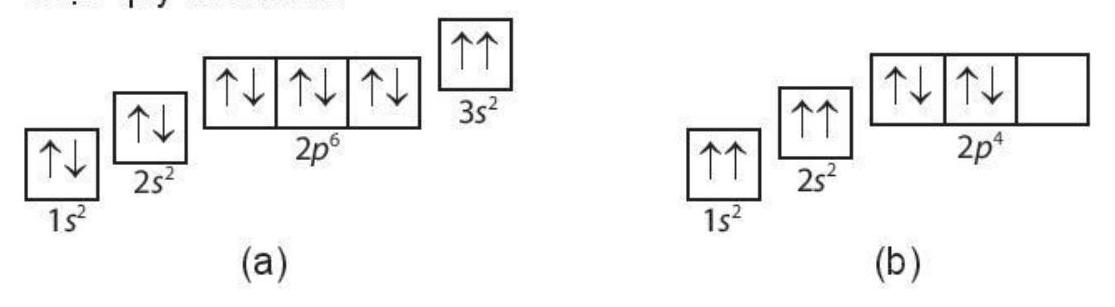
\includegraphics[max width=\textwidth, center]{2025_10_23_883c4b146e2332109fcdg-10}\\
4.12. Viết cấu hình electron của nguyên tử các nguyên tố: ${ }_{6} \mathrm{C},{ }_{8} \mathrm{O},{ }_{10} \mathrm{Ne},{ }_{11} \mathrm{Na},{ }_{13} \mathrm{Al}$, ${ }_{17} \mathrm{Cl},{ }_{29} \mathrm{Cu}$. Hãy cho biết các nguyên tố này là kim loại, phi kim hay khí hiếm.\\
4.13. Viết cấu hình electron dưới dạng ô lượng tử của các nguyên tử ${ }_{12} \mathrm{Mg}$ và ${ }_{24} \mathrm{Cr}$. Hãy cho biết các nguyên tố này là kim loại, phi kim hay khí hiếm.\\
4.14. Nguyên tố $X$ được sử dụng rộng rãi để chống đóng băng và khử băng như một chất bảo quản. Nguyên tố Y là nguyên tố thiết yếu cho các cơ thể sống, đồng thời nó được sử dụng nhiều trong việc sản xuất phân bón. Nguyên tử của nguyên tố $X$ có electron ở mức năng lượng cao nhất là $3 p$. Nguyên tử của nguyên tố $Y$ có một electron ở lớp ngoài cùng $4 s$. Nguyên tử $X$ và $Y$ có số electron hơn kém nhau là 3 . Nguyên tử $X, Y$ lần lượt là\\
A. khí hiếm và kim loại.\\
B. kim loại và khí hiếm.\\
C. kim loại và kim loại.\\
D. phi kim và kim Ioại.\\
4.15. $X$ được dùng làm chất bán dẫn trong kĩ thuật vô tuyến điện, chế tạo pin mặt trời. Nguyên tử của nguyên tố $X$ có 3 lớp electron. Lớp ngoài cùng có 4 electron. Xác định số hiệu nguyên tử của $X$ và tên nguyên tố $X$. Viết cấu hình electron của $X$.\\
4.16*. $X$ được dùng để làm vỏ phủ vệ tinh nhân tạo hay khí cầu nhằm tăng nhiệt độ nhờ có tính hấp thụ bức xạ điện từ mặt trời khá tốt. Y là một trong những thành phần để điều chế nước Javen tầy trắng quần áo, vải sợi. Nguyên tử của nguyên tố $X$ có tổng số hạt electron trong các phân lớp $p$ là 7 . Số hạt mang điện của một nguyên tử $Y$ nhiều hơn số hạt mang điện của một nguyên tử $X$ là 8 hạt. Tìm các nguyên tố $X$ và $Y$.\\
4.17*. Một nguyên tố mà nguyên tử có 4 lớp electron, có phân lớp d, lớp ngoài cùng đã bão hoà electron. Hãy tính tổng số electron $s$ và electron $p$ của nguyên tố này.\\
4.18*. A được dùng để chế tạo đèn có cường độ sáng cao. Nguyên tử A có electron ở phân lớp 3d chỉ bằng một nửa phân lớp 4s. Viết cấu hình electron của nguyên tử $A$ và tên nguyên tố $A$.\\
4.19*. Nguyên tố $A$ có cấu hình electron lớp ngoài cùng là $4 \mathrm{~s}^{1}$. Nguyên tố $B$ có phân lớp cuối là $3 p^{5}$. Viết cấu hình electron đầy đủ của $A, B$. Xác định tên $A, B$.

\section*{ÔN TẬP CHƯONG 1}
OT1.1. Nguyên tử là phần tử nhỏ nhất của chất và\\
A. không mang điện.\\
B. mang điện tích dương.\\
C. mang điện tích âm.\\
D. có thể mang điện hoặc không mang điện.

OT1.2. Phát biểu nào sau đây không đúng?\\
A. Chỉ có hạt nhân nguyên tử oxygen mới có 8 proton.\\
B. Chỉ có hạt nhận nguyên tử oxygen mới có 8 neutron.\\
C. Chỉ có nguyên tử oxygen mới có 8 electron.\\
D. CảA và C.

OT1.3. Số hiệu nguyên tử cho biết\\
A. số proton trong hạt nhân nguyên tử hoặc số đơn vị điện tích hạt nhân nguyên tử.\\
B. số electron trong lớp vỏ nguyên tử.\\
C. số thứ tự của nguyên tố trong bảng tuần hoàn.\\
D. cả $A, B$ và $C$ đều đúng.

OT1.4. Cấu hình electron nào sau đây là của nguyên tử fluorine $(Z=9)$ ?\\
A. $1 s^{2} 2 s^{2} 2 p^{3}$.\\
B. $1 s^{2} 2 s^{2} 2 p^{4}$.\\
C. $1 s^{2} 2 s^{3} 2 p^{4}$.\\
D. $1 s^{2} 2 s^{2} 2 p^{5}$.

OT1.5. Nguyên tử của nguyên tố phosphorus $(Z=15)$ có số electron độc thân là\\
A. 1 .\\
B. 2 .\\
C. 3 .\\
D. 4 .

OT1.6. Trong tự nhiên, bromine có 2 đồng vị ${ }_{35}^{79} \mathrm{Br}$ có hàm lượng $50,7 \%$ và ${ }_{35}^{81} \mathrm{Br}$ có hàm lượng $49,3 \%$. Tính nguyên tử khối trung bình của bromine.

OT1.7. Lithium trong tự nhiên có 2 đồng vị là ${ }_{3}^{7} \mathrm{Li}$ và ${ }_{3}^{6} \mathrm{Li}$. Nguyên tử khối trung bình của lithium là 6,94 . Tính thành phần phần trăm của mỗi đồng vị lithium trong tự nhiên.

OT1.8. Điện tích của electron là $-1,602 \cdot 10^{-19} \mathrm{C}$ (coulomb). Tính điện tích của hạt nhân nguyên tử carbon theo đơn vị coulomb.

OT1.9*. Hợp chất Y có công thức $\mathrm{MX}_{2}$ (là hợp chất được sử dụng làm cơ chế đánh lửa bằng bánh xe trong các dạng súng cồ), trong đó $M$ chiếm $46,67 \%$ về khối lượng. Trong hạt nhân M có số neutron nhiều hơn số proton là 4 hạt. Trong hạt nhân nguyên tử X , số neutron bằng số proton. Tổng số proton trong $\mathrm{MX}_{2}$ là 58 .\\
a) Tìm $A_{M}$ và $A_{X}$.\\
b) Xác định công thức phân tử của $\mathrm{MX}_{2}$.

OT1.10*. Hợp chất có công thức phân tử $\mathrm{M}_{2} \mathrm{X}$ (được ứng dụng trong sản xuất xi măng, phân bón) có tổng số hạt là 140. Trong đó, số hạt mang điện nhiều hơn số hạt không mang điện là 44. Số khối của nguyên tử M lớn hơn số khối của nguyên tử $X$ là 23. Tổng số hạt trong nguyên từ $M$ nhiều hơn trong nguyên tử $X$ là 34. Viết cấu hình electron của các nguyên tử $M$ và $X$. Viết công thức phân tử của hợp chất $\mathrm{M}_{2} \mathrm{X}$.

\section*{Chương 2. BẢNG TUẨN HOÀN CÁC NGUYÊN TỐ HOÁ HOC}
\section*{Bai \\
 5 CẤU TẠO BẢNG TUẦN HOÀN CÁC NGUYÊN TỐ HOÁ HỌC}
5.1. X là nguyên tố rất cần thiết cho sự chuyển hoá của calcium, phosphorus, sodium, potassium, vitamin $C$ và các vitamin nhóm B. Ơ trạng thái cơ bản, cấu hình electron lớp ngoài cùng của nguyên tử X là $3 \mathrm{~s}^{2}$. Số hiệu nguyên tử của nguyên tố X là\\
A. 12 .\\
B. 13.\\
C. 11 .\\
D. 14 .\\
5.2. Chu kì là\\
A. dãy các nguyên tố mà nguyên tử của chúng có cùng số lớp electron, được xếp theo chiều khối lượng nguyên tử tăng dần.\\
B. dãy các nguyên tố mà nguyên tử của chúng có cùng số lớp electron, được xếp theo chiều số khối tăng dần.\\
C. dãy các nguyên tố mà nguyên tử của chúng có cùng số lớp electron, được xếp theo chiều điện tích hạt nhân nguyên tử tăng dần.\\
D. dãy các nguyên tố mà nguyên tử của chúng có cùng số lớp electron, được xếp theo chiều số neutron tăng dần.\\
5.3. Nhóm nguyên tố là\\
A. tập hợp các nguyên tố mà nguyên tử có cấu hình electron giống nhau, được xếp ở cùng một cột.\\
B. tập hợp các nguyên tố mà nguyên tử có cấu hình electron gần giống nhau, do đó có tính chất hoá học giống nhau và được xếp thành một cột.\\
C. tập hợp các nguyên tố mà nguyên tử có cấu hình electron tương tự nhau, do đó có tính chất hoá học gần giống nhau và được xếp thành một cột.\\
D. tập hợp các nguyên tố mà nguyên tử có tính chất hoá học giống nhau và được xếp cùng một cột.\\
5.4. Trong bảng tuần hoàn, các nguyên tố được sắp xếp không theo nguyên tắc nào?\\
A. Theo chiều tăng của điện tích hạt nhân.\\
B. Các nguyên tố có cùng số lớp electron trong nguyên tử được xếp thành một hàng.\\
C. Các nguyên tố có cùng số electron hoá trị trong nguyên tử được xếp thành một cột.\\
D. Theo chiều tăng khối lượng nguyên tử.\\
5.5. Sulfur dạng kem bôi được sử dụng để điều trị mụn trứng cá. Nguyên tử sulfur có phân lớp electron ngoài cùng là $3 \mathrm{p}^{4}$. Phát biểu nào sau đây là sai khi nói về nguyên tử sulfur?\\
A. Lớp ngoài cùng của sulfur có 6 electron.\\
B. Hạt nhân nguyên tử sulfur có 16 electron.\\
C. Trong bảng tuần hoàn sulfur nằm ở chu kì 3 .\\
D. Sulfur nằm ở nhóm VIA.\\
5.6. Hãy cho biết ý nghĩa của các thông tin có trong ô nguyên tố sau:\\
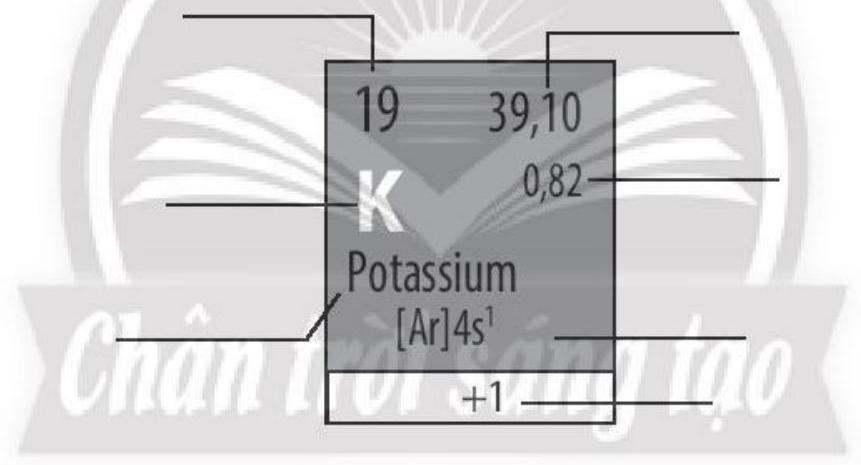
\includegraphics[max width=\textwidth, center]{2025_10_23_883c4b146e2332109fcdg-15}\\
5.7. Sử dụng bảng tuần hoàn các nguyên tố hoá học trong SGK (Hình 5.2 trang 37), hoàn thành những thông tin còn thiếu trong bảng sau:

\begin{center}
\begin{tabular}{|l|l|l|l|}
\hline
Hợp chất & Khối lượng Fe (g) & Khối lượng O (g) & Tỉ lệ khối lượng O : Fe \\
\hline
FeO &  &  &  \\
\hline
$\mathrm{Fe}_{2} \mathrm{O}_{3}$ &  &  &  \\
\hline
$\mathrm{Fe}_{3} \mathrm{O}_{4}$ &  &  &  \\
\hline
\end{tabular}
\end{center}

5.8. Hãy giải thích vì sao chu kì 3 chỉ có 8 nguyên tố.\\
5.9. Xác định vị trí của nguyên tố (ô, chu kì và nhóm) của nguyên tố có\\
a) số hiệu nguyên tử là 20 , là nguyên tố giúp xương chắc khoẻ, phòng ngừa những bệnh loãng xương, giảm tình trạng đau nhức và khó khăn trong vận động, làm nhanh lành các vết nứt gãy trên xương.\\
b) 9 electron, được sử dụng để điều chế một số dẫn xuất hydrocarbon, làm sản phẩm trung gian để sản xuất ra chất dẻo.\\
c) 28 proton, được dùng trong việc chế tạo hợp kim chống ăn mòn.\\
d) số khối là 52 và 28 neutron, dùng chế tạo thép không gỉ.\\
5.10. Viết cấu hình electron nguyên đử của các nguyên tố và xác định tên nguyên tố:\\
a) Chu kì 3 , nhóm IIIA, được dùng trong ngành công nghiệp chế tạo, cụ thể là tạo ra các chi tiết cho xe ô tô, xe tải, tàu hoả, tàu biển và cả máy bay.\\
b) Chu kì 4 , nhóm IB, được sử dụng rất nhiều trong sản xuất các nguyên liệu như dây điện, que hàn, tay cầm, các đồ dùng nội thất trong nhà, các tượng đúc, nam châm điện từ, các động cơ máy móc, ...\\
5.11. Một hợp chất có công thức $X Y_{2}$, trong đó $X$ chiếm $50 \%$ về khối lượng. Trong hạt nhân của $X$ và $Y$ đều có số proton bằng số neutron. Tổng số proton trong phân tử $X Y_{2}$ là 32. Hợp chất này được sử dụng như chất trung gian để sản xuất sulfuric acid.\\
a) Viết cấu hình electron của $X$ và $Y$.\\
b) Xác định vị trí của $X$ và $Y$ trong bảng tuần hoàn và công thức phân tử hợp chất $X Y_{2}$.\\
5.12. Hai nguyên tố $X$ và $Y$ đứng kế tiếp nhau trong cùng một chu kì, có tổng số điện tích hạt nhân bằng 25.\\
a) Hãy viết cấu hình electron của nguyên tử $X, Y$.\\
b) Xác định vị trí của $X, Y$ trong bảng tuần hoàn và tên nguyên tố $X, Y$.\\
5.13. $X, Y$ là hai nguyên tố thuộc cùng nhóm $A$ ở hai chu kì liên tiếp trong bảng tuần hoàn, có tổng số proton trong hai hạt nhân là 32. Viết cấu hình electron của nguyên tử $X$ và $Y$. Xác định tên $X, Y$.\\
5.14*. $X$ và $Y$ là hai nguyên tố thuộc chu kì nhỏ, thuộc hai nhóm $A$ kế tiếp nhau trong bảng tuần hoàn. Ở trạng thái đơn chất, $X$ và $Y$ phản ứng được với nhau. Tổng số proton trong hạt nhân nguyên tử của $X$ và $Y$ là 23. Biết rằng $X$ đứng sau $Y$ trong bảng tuần hoàn. Xác định tên nguyên tố $X, Y$.\\
5.15*. Hoà tan hoàn toàn 6,645 gam hỗn hợp muối chloride của hai kim loại kiềm thuộc hai chu kì kế tiếp nhau vào nước được dung dịch $X$. Cho toàn bộ dung dịch $X$ tác dụng hoàn toàn với dung dịch $\mathrm{AgNO}_{3}(\mathrm{du})$, thu được 18,655 gam kết tủa. Xác định 2 kim loại kiềm.

\section*{XU HUỚNG BIẾN ĐỔI MỘT SỐ TÍNH CHẤT CỦA NGUYÊN TỬ CÁC NGUYÊN TỐ, THÀNH PHẦN VÀ MỘT SỐ TÍNH CHẤT CỦA HỢ CHẤT TRONG MỘT CHU Kİ VÀ NHÓM}
6.1. Dãy nguyên tố nào sau đây sắp xếp theo chiều tăng dần của bán kính nguyên tử?\\
A. Be, F, O, C, Mg.\\
B. $\mathrm{Mg}, \mathrm{Be}, \mathrm{C}, \mathrm{O}, \mathrm{F}$.\\
C. F, O, C, Be, Mg.\\
D. F, Be, C, Mg, O.\\
6.2. Nguyên tử của nguyên tố nào có bán kính lớn nhất trong các nguyên tử sau đây?\\
A. Al.\\
B. P.\\
C. S.\\
D. K.\\
6.3. Dãy nguyên tố nào sau đây sắp xếp theo chiều tăng dần độ âm điện của nguyên tử?\\
A. Li, F, N, Na, C.\\
B. F, Li, Na, C, N.\\
C. Na, Li, C, N, F.\\
D. N, F, Li, C, Na.\\
6.4. Nguyên tử của nguyên tố nào sau đây có độ âm điện lớn nhất? Cho biết nguyên tố này được sử dụng trong công nghệ hàn, sản xuất thép và methanol.\\
A. B.\\
B. N.\\
C. O.\\
D. Mg.\\
6.5. Nguyên tử của nguyên tố nào sau đây có tính kim loại mạnh nhất? Cho biết nguyên tố này được sử dụng trong đồng hồ nguyên tử, với độ chính xác ở mức giây trong hàng nghìn năm.\\
A. Hydrogen.\\
B. Beryllium.\\
C. Caesium.\\
D. Phosphorus.\\
6.6. Nguyên tử của nguyên tố nào sau đây có tính phi kim mạnh nhất? Cho biết nguyên tố này có trong thành phần của hợp chất teflon, được sử dụng để tráng chảo chống dính.\\
A. Fluorine.\\
B. Bromine.\\
C. Phosphorus.\\
D. Iodine.\\
6.7. Hydroxide nào có tính base mạnh nhất trong các hydroxide sau đây? Cho biết hợp chất này được sử dụng làm chất phụ gia cho dầu bôi trơn của động cơ đốt trong.\\
A. Calcium hydroxide.\\
B. Barium hydroxide.\\
C. Strontium hydroxide.\\
D. Magnesium hydroxide.\\
6.8. Hydroxide nào có tính acid mạnh nhất trong các hydroxide sau đây? Cho biết hợp chất này được dùng để phân huỷ các quặng phức tạp; phân tích khoáng vật hoặc làm chất xúc tác.\\
A. Silicic acid.\\
B. Sulfuric acid.\\
C. Phosphoric acid.\\
D. Perchloric acid.\\
6.9. Cho các nguyên tố $X, Y, Z$ với số hiệu nguyên tử lần lượt là 4, 12, 20. Phát biểu nào sau đây sai?\\
A. Các nguyên tố này đều là các kim loại mạnh nhất trong chu kì.\\
B. Các nguyên tố này không cùng thuộc một chu kì.\\
C. Thứ tự tăng dần tính base là: $\mathrm{X}(\mathrm{OH})_{2}, \mathrm{Y}(\mathrm{OH})_{2}, \mathrm{Z}(\mathrm{OH})_{2}$.\\
D. Thứ tự tăng dần độ âm điện là: $Z, Y, X$.\\
6.10. Hãy cho biết:\\
a) Sự biến đổi tính kim loại và tính phi kim của nguyên tử một nguyên tố.\\
b) Quan hệ giữa tính phi kim và độ âm điện của nguyên tử một nguyên tố.\\
c) Quan hệ giữa sự biến đổi độ âm điện và tính phi kim của nguyên tử các nguyên tố nhóm A trong bảng tuần hoàn.\\
6.11. Quan sát hình sau:

\section*{$\begin{array}{lll}\text { A } & \text { B } & \text { C }\end{array}$}
3 quả cầu $A, B, C$ tượng trưng cho nguyên tử các nguyên tố helium, krypton và radon. Quả cầu nào là krypton?\\
6.12. Sắp xếp các nguyên tử sau đây theo thứ tự tăng dần độ âm điện: $\mathrm{Cl}, \mathrm{Al}, \mathrm{Na}$, P, F.\\
6.13. Sắp xếp các nguyên tử sau đây theo thứ tự giảm dần tính kim loại: Na, AI, $\mathrm{Si}, \mathrm{Mg}, \mathrm{P}, \mathrm{Cl}, \mathrm{S}, \mathrm{F}$.\\
6.14. Viết phương trình phản ứng của các chất sau với nước (nếu có): $\mathrm{Na}_{2} \mathrm{O}, \mathrm{SO}_{3}$, $\mathrm{Cl}_{2} \mathrm{O}_{7}, \mathrm{CO}_{2}, \mathrm{CaO}, \mathrm{N}_{2} \mathrm{O}_{5}$. Nhận xét về tính base, tính acid của các sản phẩm tạo thành.\\
6.15*. Dựa vào Hình 6.1 và Bảng 6.1 trong SGK, hãy vẽ đồ thị hoặc biểu đồ đối với hai đại lượng bán kính nguyên tử và độ âm điện trong bảng số liệu trên. Quan sát và cho biết hai đại lượng này biến thiên như thế nào. Giải thích.

\section*{ĐINH LUẬT TUẦN HOÀN Ý NGHĨA CỦA BẢNG TUẦN HOÀN CÁC NGUYÊN TỐ HOÁ HỌC}
7.1. Cấu hình electron nguyên tử iron: $[\mathrm{Ar}] 3 \mathrm{~d}^{6} 4 \mathrm{~s}^{2}$. Iron ở\\
A. ô 26, chu kì 4, nhóm VIIIA.\\
B. ô 26, chu kì 4, nhóm VIIIB.\\
C. ô 26, chu kì 4, nhóm IIA.\\
D. ô 26 , chu kì 4 , nhóm IIB.\\
7.2. Nguyên tố $X$ có số hiệu nguyên tử là 8 .\\
a) Nguyên tử của nguyên tố $X$ có cấu hình electron là\\
A. $1 s^{2} 2 s^{2} 2 p^{3}$.\\
B. $1 s^{2} 2 s^{1} 2 p^{5}$.\\
C. $1 s^{1} 2 s^{2} 2 p^{5}$.\\
D. $1 s^{2} 2 s^{2} 2 p^{4}$.\\
b) Nguyên tố $X$ thuộc chu kì\\
A. 1 .\\
B. 2 .\\
C. 3 .\\
D. 4 .\\
c) Nguyên tố $X$ thuộc nhóm\\
A. VIIIB.\\
B. VIB.\\
C. VIIA.\\
D. VIA.\\
7.3. Nguyên tố $X$ thuộc chu kì 3 , nhóm IIA. Nguyên tử của nguyên tố $X$ có cấu hình electron là\\
A. $1 s^{2} 2 s^{2} 2 p^{6} 3 s^{1}$.\\
B. $1 s^{2} 2 s^{2} 2 p^{6}$.\\
C. $1 s^{2} 2 s^{2} 2 p^{5} 3 s^{4}$.\\
D. $1 s^{2} 2 s^{2} 2 p^{6} 3 s^{2}$.\\
7.4. Nguyên tử của nguyên tố $X$ có cấu hình electron: $1 s^{2} 2 s^{2} 2 p^{6} 3 s^{2} 3 p^{3}$.\\
a) Số electron lớp ngoài cùng của $X$ là\\
A. 3 .\\
B. 2.\\
C. 6 .\\
D. 5 .\\
b) $X$ thuộc chu kì\\
A. 1 .\\
B. 2.\\
C. 3 .\\
D. 4 .\\
c) X thuộc nhóm\\
A. IA.\\
B. VA.\\
C. IIIA.\\
D. IVA.\\
7.5. Phosphorus được dùng vào mục đích quân sự như sản xuất bom, đạn cháy, đạn khói. Nguyên tố phosphorus ở ô số 15 , chu kì 3 , nhóm VA trong bảng tuần hoàn. Hãy cho biết:

\begin{itemize}
  \item Cấu hình electron của phosphorus.
  \item Số electron lớp ngoài cùng của nguyên tử phosphorus.
  \item Phosphorus là kim loại hay phi kim.
  \item Công thức oxide cao nhất của phosphorus.
  \item Công thức hợp chất khí của phosphorus với hydrogen.
  \item Công thức hydroxide cao nhất của phosphorus.
  \item Oxide và hydroxide cao nhất của phosphorus có tính acid hay base.\\
7.6. Hợp chất khí với hydrogen của nguyên tố X có công thức $\mathrm{XH}_{4}$, được sử dụng làm tác nhân ghép nối để bám dính các sợi như sợi thuỷ tinh và sợi carbon. Oxide cao nhất của $X$ chứa $53,3 \%$ oxygen về khối lượng, thường được dùng để sản xuất kính cửa sồ, lọ thuỷ tinh.\\
a) Tính nguyên tử khối của $X$.\\
b) $X$ là nguyên tố nào?\\
7.7. Một nguyên tố tạo hợp chất khí với hydrogen có công thức $\mathrm{RH}_{3}$, được sử dụng để trung hoà các thành phần acid của dầu thô, bảo vệ thiết bị không bị ăn mòn trong ngành công nghiệp dầu khí. Nguyên tố này chiếm $25,93 \%$ về khối lượng trong oxide cao nhất. Xác định tên nguyên tố.\\
7.8. Oxide cao nhất của nguyên tố R thuộc nhóm VIA có $60 \%$ oxygen về khối lượng, là một sản phẩm trung gian để sản xuất acid $\mathrm{H}_{2} \mathrm{SO}_{4}$ có tầm quan trọng bậc nhất trong công nghiệp. Hãy xác định nguyên tố $R$ và viết công thức oxide cao nhất.\\
7.9 Oxide cao nhất của nguyên tố $R$ có dạng $R_{2} O_{5}$, được sử dụng làm chất hút ẩm cho chất lỏng và khí. Hợp chất của $R$ với hydrogen ở thể khí có chứa $8,82 \%$ hydrogen về khối lượng, là khí rất độc, gây chết với các triệu chứng khó hô hấp, đau đầu, chóng mặt, buồn nôn. Xác định công thức phân tử của hợp chất khí của $R$ với hydrogen.\\
7.10*. Oxide cao nhất của một nguyên tố $R$ chứa $72,73 \%$ oxygen. Tuy không phải là khí quá độc nhưng với nồng độ lớn thì sẽ làm giảm nồng độ oxygen trong không khí, gây ra các tác hại như mệt mỏi, khó thở, kích thích thần kinh, tăng nhịp tim và các rối loạn khác. Hợp chất khí với hydrogen chứa $75 \%$ nguyên tố đó. Hợp chất này thường được sử dụng làm nhiên liệu cho các lò nướng, nhà cửa, máy nước nóng, lò nung, xe ô tô. Viết công thức oxide cao nhất và hợp chất khí với hydrogen của nguyên tố $R$.
\end{itemize}

\section*{ÔN TẬP CHƯONG 2}
OT2.1. Sắt (iron) là vật liệu dùng làm bộ khung cho các công trình xây dựng, các khung giàn cho các loại cầu vượt, cầu bắc qua sông, cầu đi bộ, ... Nguyên tố sắt nằm ở ô 26 trong bảng tuần hoàn. Cấu hình electron của nguyên tử iron là\\
A. $1 s^{2} 2 s^{2} 2 p^{6} 3 s^{2} 3 p^{6} 3 d^{6} 4 s^{2}$.\\
B. $1 s^{2} 2 s^{2} 2 p^{6} 3 s^{2} 3 p^{6} 3 d^{8}$.\\
C. $1 s^{2} 2 s^{2} 2 p^{6} 3 s^{2} 3 p^{6} 4 s^{2} 4 p^{6}$.\\
D. $1 s^{2} 2 s^{2} 2 p^{6} 3 s^{2} 3 p^{6} 3 d^{7} 4 s^{1}$.

OT2.2. Các muối của nguyên tố chromium được dùng trong ngành thuộc da, làm phụ gia cho xăng, chất nhuộm màu xanh lục hay màu hồng ngọc cho đồ gốm, trang thiết bị trong dàn khoan, thuốc nhuộm, sơn và chất vệ sinh cho đồ dùng thuỷ tinh trong phòng thí nghiệm. Nguyên tử nguyên tố Cr có cấu hình $1 s^{2} 2 s^{2} 2 p^{6} 3 s^{2} 3 p^{6} 3 d^{5} 4 s^{1}$. Vị trí của nguyên tố Cr trong bảng tuần hoàn:\\
A. ô 24 , chu kì 3 , nhóm IA.\\
B. ô 24 , chu kì 4 , nhóm VIB.\\
C. ô 24, chu kì 4, nhóm VIA.\\
D. ô 24 , chu kì 4 , nhóm IB.

Dữ kiện sử dụng cho OT2.3 và OT2.4. Cho các nguyên tố: Ca, C, F, O, Be.\\
OT2.3. Dãy các nguyên tố nào sau đây sắp xếp theo chiều tăng dần độ âm điện của nguyên tử?\\
A. C, F, Ca, O, Be.\\
B. $\mathrm{Ca}, \mathrm{Be}, \mathrm{C}, \mathrm{O}, \mathrm{F}$.\\
C. F, O, C, Be, Ca.\\
D. O, C, F, Ca, Be.

OT2.4. Dãy các nguyên tố nào sau đây sắp xếp theo chiều tăng dần bán kính nguyên tử?\\
A. C, F, Ca, O, Be.\\
B. $\mathrm{Ca}, \mathrm{Be}, \mathrm{C}, \mathrm{O}, \mathrm{F}$.\\
C. $F, O, C, B e, C a$.\\
D. O, C, F, Ca, Be.

OT2.5. Silicon được dùng trong công nghệ sản xuất chip máy tính hiện đại. Aluminium được dùng đề làm vỏ phủ vệ tinh nhân tạo hay khí cầu nhằm tăng nhiệt độ nhờ nó có tính hấp thụ bức xạ điện từ Mặt Trời khá tốt. Phosphorus là một khoáng chất thiết yếu đối với sự phát triển của xương và răng. Hãy so sánh tính phi kim của $\mathrm{Si}, \mathrm{Al}$ và P .

OT2.6. Sodium hydroxide được ứng dụng trong khâu loại bỏ acid béo để tinh chế dầu thực vật, động vật trước khi dùng để sản xuất thực phẩm. Magnesium hydroxide là một thành phần phổ biến của các thuốc kháng acid cũng như các thuốc nhuận tràng. Aluminium hydroxide được dùng trong sản xuất gốm sứ, thuỷ tinh và sản xuất giấy. So sánh tính base của $\mathrm{NaOH}, \mathrm{Mg}(\mathrm{OH})_{2}, \mathrm{Al}(\mathrm{OH})_{3}$.

OT2.7. Oxide cao nhất của một nguyên tố là $\mathrm{RO}_{3}$. Nó có trong thành phần của oleum, được sử dụng trong sản xuất nhiều chất nổ. Trong hợp chất khí của R với hydrogen có $5,88 \%$ hydrogen về khối lượng. Xác định nguyên tố $R$.

OT2.8. Hợp chất khí với hydrogen của nguyên tố R là $\mathrm{RH}_{4}$. Oxide cao nhất của R chứa $53,3 \%$ oxygen về khối lượng. Oxide này được sử dụng trong ngành xây dựng, như sản xuất bê tông. Tìm nguyên tố $R$.

OT2.9*. Trong sản xuất thịt chế biến sẵn, người ta thường bổ sung một hợp chất có công thức dạng $X_{2} Y$ để ức chế sự sinh sôi phát triển của vi khuẩn trong thịt, giúp thịt lâu hư, tránh các trường hợp ngộ độc thực phẩm do thịt bị ôi thiu. Phân tử $X_{2} Y$ có tổng số proton là 23 . Biết $X, Y$ ở hai nhóm $A$ liên tiếp trong cùng một chu kì. Tìm công thức phân tử của $X_{2} Y$.

OT2.10*. Có hai nguyên tố $X, Y$ thuộc cùng nhóm và ở hai chu kì liên tiếp, tổng số đơn vị điện tích hạt nhân của $X$ và $Y$ là 58. Trong đó, một nguyên tố đóng vai trò quan trọng đối với hệ thần kinh, đặc biệt ở người già thiếu chất này dễ bị suy nhược thần kinh, trí nhớ kém, tinh thần không ổn định, đau đầu. Oxide của nguyên tố còn lại nhờ tính ổn định nhiệt cao nên được ứng dụng nhiều trong ngành công nghiệp gốm sứ, thuỷ tinh và quang học. Xác định $\mathrm{X}, \mathrm{Y}$.

\section*{Chương 3. LIÊN KẾT HOÁ HỌC}
\section*{Bai}
\section*{8 QUY TẮC OCTET}
8.1. Vì sao các nguyên tử lại liên kết với nhau thành phân tử?\\
A. Để mỗi nguyên tử trong phân tử đạt được cơ cấu electron ổn định, bền vững.\\
B. Để mỗi nguyên tử trong phân tử đều đạt 8 electron ở lớp ngoài cùng.\\
C. Để tổng số electron ngoài cùng của các nguyên tử trong phân tử là 8 .\\
D. Để lớp ngoài cùng của mỗi nguyên tử trong phân tử có nhiều electron độc thân nhất.\\
8.2. Nguyên tử nào sau đây có khuynh hướng đạt cấu hình electron bền của khí hiếm neon khi tham gia hình thành liên kết hoá học?\\
A. Chlorine.\\
B. Sulfur.\\
C. Oxygen.\\
D. Hydrogen.\\
8.3. Sodium hydride $(\mathrm{NaH})$ là một hợp chất được sử dụng như một chất Iưu trữ hydrogen trong các phương tiện chạy bằng pin nhiên liệu do khả năng giải phóng hydrogen của nó. Trong sodium hydride, nguyên tử sodium có cấu hình electron bền của khí hiếm\\
A. helium.\\
B. argon.\\
C. krypton.\\
D. neon.\\
8.4. Khi tham gia hình thành liên kết hoá học, các nguyên tử lithium và chlorine có khuynh hướng đạt cấu hình electron bền của lần lượt các khí hiếm nào dưới đây?\\
A. Helium và argon.\\
B. Helium và neon.\\
C. Neon và argon.\\
D. Argon và helium.\\
8.5. Trong phân tử HBr , nguyên tử hydrogen và bromine đã lần lượt đạt cấu hình electron bền của các khí hiếm nào dưới đây?\\
A. Neon và argon.\\
B. Helium và xenon.\\
C. Helium và radon.\\
D. Helium và krypton.\\
8.6. Trong các hợp chất, nguyên tử magnesium đã đạt được cấu hình bền của khí hiếm gần nhất bằng cách\\
A. cho đi 2 electron.\\
B. nhận vào 1 electron.\\
C. cho đi 3 electron.\\
D. nhận vào 2 electron.\\
8.7. Cho các phân tử sau: $\mathrm{Cl}_{2}, \mathrm{H}_{2} \mathrm{O}, \mathrm{NaF}$ và $\mathrm{CH}_{4}$. Có bao nhiêu nguyên tử trong các phân tử trên đạt cấu hình electron bền của khí hiếm neon?\\
A. 3 .\\
B. 2 .\\
C. 5.\\
D. 4 .\\
8.8. Nguyên tử trong phân tử nào dưới đây ngoại lệ với quy tắc octet?\\
A. $\mathrm{H}_{2} \mathrm{O}$.\\
B. $\mathrm{NH}_{3}$.\\
C. HCl .\\
D. $\mathrm{BF}_{3}$.\\
8.9. Em hãy nêu tên và công thức hoá học của 1 chất ở thể rắn, 1 chất ở thể lỏng và 1 chất ở thể khí (trong điều kiện thường), trong đó nguyên tử oxygen đạt được cấu hình bền của khí hiếm neon.\\
8.10. Potassium iodide (KI) được sử dụng như một loại thuốc long đờm, giúp làm lỏng và phá vỡ chất nhầy trong đường thở, thường dùng cho các bệnh nhân hen suyễn, viêm phế quản mãn tính. Trong trường hợp bị nhiễm phóng xạ, KI còn giúp ngăn tuyến giáp hấp thụ iodine phóng xạ, bảo vệ và giảm nguy cơ ung thư tuyến giáp. Trong phân tử KI , các nguyên tử K và I đều đã đạt được cơ cấu bền của khí hiếm gần nhất. Đó lần lượt là những khí hiếm nào?

\section*{Baii 9 LIÊN KẾT ION}
9.1. Điều nào dưới đây đúng khi nói về ion $\mathrm{S}^{2-}$ ?\\
A. Có chứa 18 proton.\\
B. Có chứa 18 electron.\\
C. Trung hoà về điện.\\
D. Được tạo thành khi nguyên tử sulfur ( S ) nhận vào 2 proton.\\
9.2. Điều nào dưới đây không đúng khi nói về hợp chất sodium oxide ( $\mathrm{Na}_{2} \mathrm{O}$ )?\\
A. Trong phân tử $\mathrm{Na}_{2} \mathrm{O}$, các ion sodium $\mathrm{Na}^{+}$và ion oxide $\mathrm{O}^{2-}$ đều đạt cấu hình electron bền vững của khí hiếm neon.\\
B. Phân tử $\mathrm{Na}_{2} \mathrm{O}$ tạo bởi lực hút tĩnh điện giữa hai ion $\mathrm{Na}^{+}$và một ion $\mathrm{O}^{2-}$.\\
C. Là chất rắn trong điều kiện thường.\\
D. Không tan trong nước, chỉ tan trong dung môi không phân cực như benzene, carbon tetrachloride, ...\\
9.3. Tính chất nào dưới đây đúng khi nói về hợp chất ion?\\
A. Hợp chất ion có nhiệt độ nóng chảy thấp.\\
B. Hợp chất ion tan tốt trong dung môi không phân cực.\\
C. Hợp chất ion có cấu trúc tinh thể.\\
D. Hợp chất ion dẫn điện ở trạng thái rắn.\\
9.4. Hợp chất A có các tính chất sau: Ở thể rắn trong điều kiện thường, dể tan trong nước tạo dung dịch dẫn điện được. Hợp chất A là\\
A. sodium chloride.\\
B. glucose.\\
C. sucrose.\\
D. fructose.\\
9.5. Tính chất nào sau đây không phải của magnesium oxide ( MgO )?\\
A. Có nhiệt độ nóng chảy cao hơn so với NaCl .\\
B. Chất khí ở điều kiện thường.\\
C. Có cấu trúc tinh thể.\\
D. Phân tử tạo bởi lực hút tĩnh điện giữa ion $\mathrm{Mg}^{2+}$ và $\mathrm{O}^{2-}$.\\
9.6. Sodium sulfide $\left(\mathrm{Na}_{2} \mathrm{~S}\right)$ là một hợp chất hoá học được sử dụng trong ngành công nghiệp giấy và bột giấy, xử lí nước, công nghiệp dệt may và các quy trình sản xuất hoá chất khác như sản xuất cao su, thuốc nhuộm lưu huỳnh và thu hồi dầu, ... Điều thú vị là sodium sulfide đã được chứng minh là có vai trò trong bảo vệ tim mạch, chống lại chứng thiếu máu cục bộ ở tim và giúp bảo vệ phổi, chống lại tổn thương phổi do máy thở. Trình bày sự tạo thành sodium sulfide khi cho sodium phản ứng với sulfur.\\
9.7. Chỉ ra cấu trúc đúng của ô mạng tinh thể sodium chloride:\\
A.\\
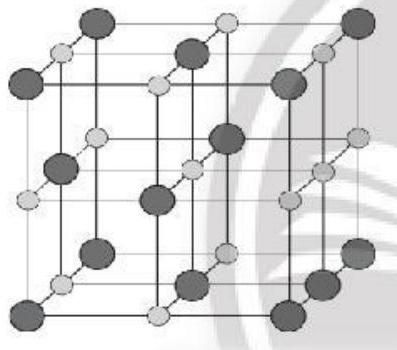
\includegraphics[max width=\textwidth, center]{2025_10_23_883c4b146e2332109fcdg-26(1)}\\
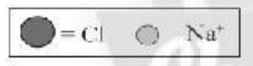
\includegraphics[max width=\textwidth, center]{2025_10_23_883c4b146e2332109fcdg-26}\\
B.\\
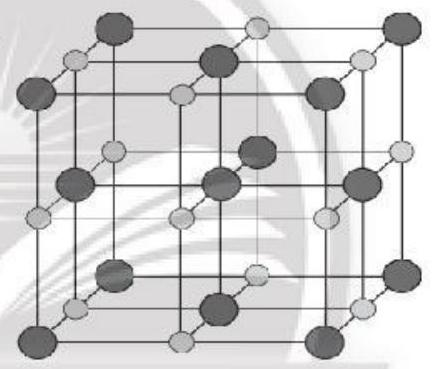
\includegraphics[max width=\textwidth, center]{2025_10_23_883c4b146e2332109fcdg-26(3)}\\
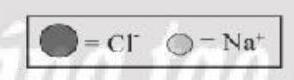
\includegraphics[max width=\textwidth, center]{2025_10_23_883c4b146e2332109fcdg-26(2)}\\
C.\\
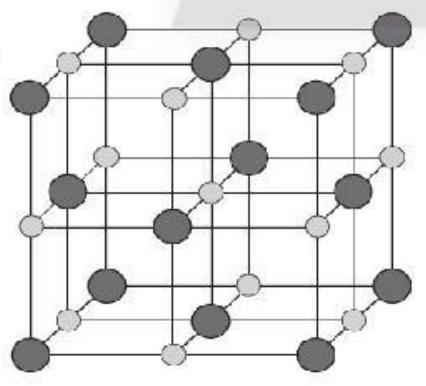
\includegraphics[max width=\textwidth, center]{2025_10_23_883c4b146e2332109fcdg-26(4)}\\
$-\mathrm{Cl}^{-} \quad \mathrm{O}=\mathrm{Na}^{+}$\\
D.\\
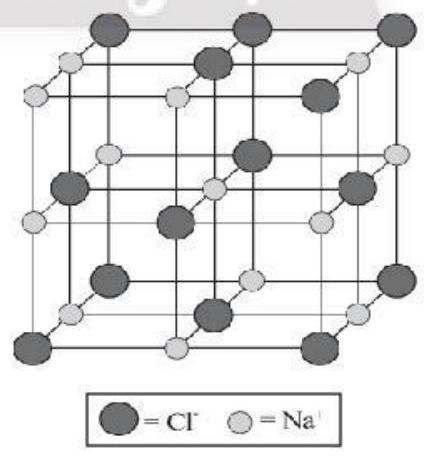
\includegraphics[max width=\textwidth, center]{2025_10_23_883c4b146e2332109fcdg-26(5)}\\
9.8. Magnesium chloride là một chất xúc tác phổ biến trong hoá học hữu cơ. Trình bày sự hình thành phân tử $\mathrm{MgCl}_{2}$ khi cho magnesium tác dụng với chlorine.\\
9.9. Trong đời sống, muối ăn ( NaCl ) và các gia vị, phụ gia ( $\mathrm{C}_{5} \mathrm{H}_{8} \mathrm{NO}_{4} \mathrm{Na}$ : bột ngọt; $\mathrm{C}_{7} \mathrm{H}_{5} \mathrm{O}_{2} \mathrm{Na}$ : chất bảo quản thực phẩm) đều có chứa ion sodium. Hiệp hội Tim mạch Hoa Kỳ khuyến cáo các cá nhân nên hạn chế lượng sodium xuống dưới 2300 mg mỗi ngày vì nếu tiêu thụ nhiều hơn sẽ ảnh hưởng đến tim mạch và thận. Nếu trung bình mỗi ngày, một người dùng tổng cộng 5,0 gam muối ăn; 0,5 gam bột ngọt và 0,05 gam chất bảo quản thì lượng sodium tiêu thụ có vượt mức giới hạn cho phép nói trên không?\\
9.10. Trình bày cách vẽ một ô mạng tinh thể NaCl .\\
9.11*. Biểu đồ dưới đây cho biết mối quan hệ giữa năng lượng của hệ các ion trái dấu so với khoảng cách giữa chúng:\\
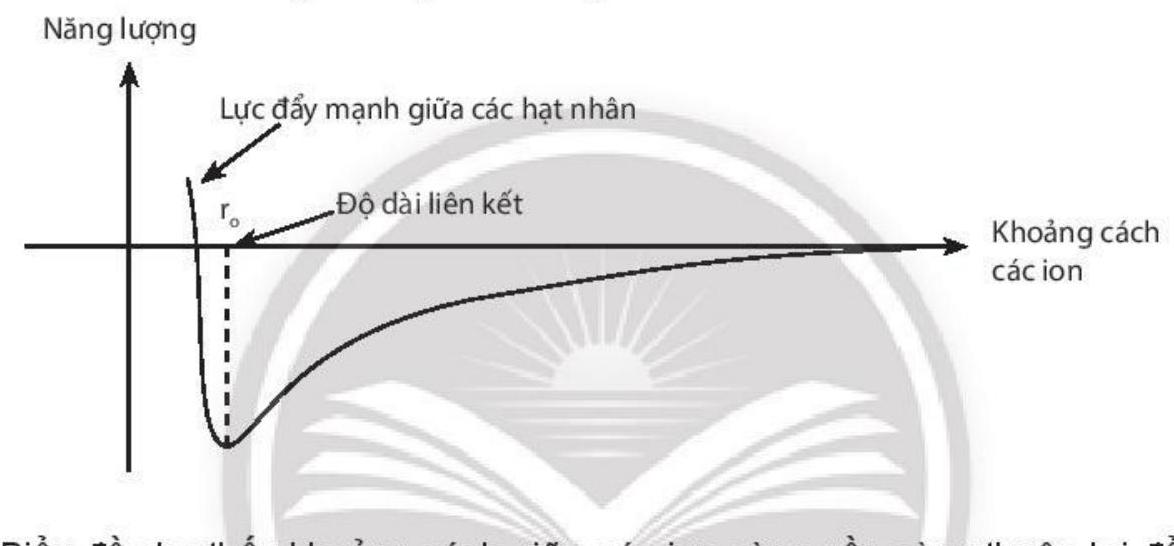
\includegraphics[max width=\textwidth, center]{2025_10_23_883c4b146e2332109fcdg-27}

Biểu đồ cho thấy khoảng cách giữa các ion càng gần càng thuận lợi để hệ đạt được trạng thái năng lượng tối thiểu (bền vững). Tuy nhiên, ở khoảng cách nhỏ quá, các ion lại đẩy nhau do hạt nhân của các ion đều mang điện tích dương.\\
Năng lượng tối thiểu đại diện cho độ bền liên kết và khoảng cách $r_{\circ}$ tại mức năng lượng tối thiểu gọi là độ dài liên kết. Bằng cách thực hiện một loạt các phép tính, người ta thấy rằng các hợp chất ion được hình thành bởi các ion có điện tích lớn hơn sẽ tạo ra liên kết mạnh hơn và các hợp chất ion có độ dài liên kết ngắn hơn sẽ hình thành liên kết mạnh hơn.\\
Sử dụng nhận định trên để dự đoán và giải thích độ bền liên kết giữa các hợp chất ion sau:\\
a) NaCl và $\mathrm{Na}_{2} \mathrm{O}$.\\
b) NaCl và NaF .\\
9.12*. $\mathrm{X}, \mathrm{Y}, \mathrm{Z}$ là các hợp chất ion thuộc trong số các chất sau: $\mathrm{NaF}, \mathrm{MgO}$ và $\mathrm{MgCl}_{2}$. Nhiệt độ nóng chảy của các hợp chất $X, Y, Z$ được thể hiện qua biểu đồ:\\
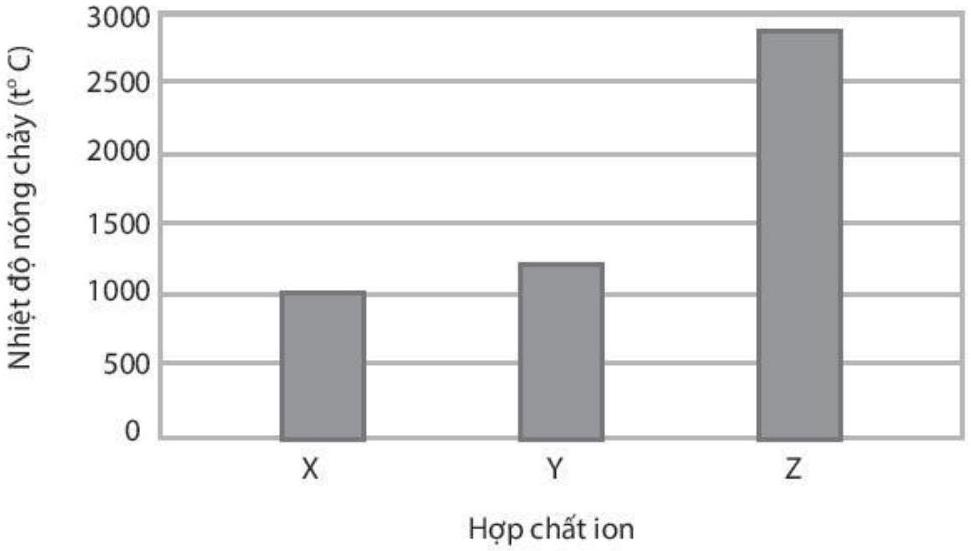
\includegraphics[max width=\textwidth, center]{2025_10_23_883c4b146e2332109fcdg-28}

Trình bày cách xác định các chất $X, Y, Z$.\\
9.13. Cho biết lực hút tĩnh điện được tính theo công thức sau: $F=k \frac{\left|q_{1}\right|\left|q_{2}\right|}{r^{2}}\left(q_{1}\right.$, $\mathrm{q}_{2}$ là giá trị điện tích của hai điện tích điểm, đơn vị là C (coulomb); r là khoảng cách giữa hai điện tích điểm, đơn vị là m (meter); $k$ là hằng số coulomb). Dựa vào công thức trên, hãy so sánh gần đúng lực hút tĩnh điện giữa các ion trái dấu trong phân tử NaCl và phân tử MgO . Từ đó, cho biết nhiệt độ nóng chảy và nhiệt độ sôi của hợp chất nào cao hơn.\\
9.14. Hình dạng và cấu trúc tinh thể của mọi hợp chất ion có giống nhau không? Giải thích.\\
9.15. Vì sao các hợp chất ion thường tồn tại ở trạng thái rắn và cứng trong điều kiện thường, nhưng lại giòn, dễ vỡ?\\
9.16. Vì sao nói sodium chloride có cấu trúc mạng tinh thể kiểu lập phương tâm diện?

\section*{LIÊN KẾT CộNG HOÁ TRỊ}
10.1. Trong phân tử ammonia $\left(\mathrm{NH}_{3}\right)$, số cặp electron chung giữa nguyên tử nitrogen và các nguyên tử hydrogen là\\
A. 3 .\\
B. 2 .\\
C. 1.\\
D. 4 .\\
10.2. Biết nguyên tử chlorine có 7 electron hoá trị, công thức electron của phân tử chlorine là\\
A.\\
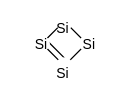
\includegraphics{smile-fceb65d9546d5a894720e73ad67bc570d357c4c2}\\
B. : $\ddot{C}|:: \ddot{C}|$ :\\
C. :CÄ::Cöl:\\
D.\\
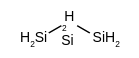
\includegraphics{smile-e90efded0fc5444409a710e3e1a693a3ef80a076}\\
10.3. Chất nào sau đây không có liên kết cộng hoá trị phân cực?\\
A. $\mathrm{O}_{2}$.\\
B. $\mathrm{CO}_{2}$.\\
C. $\mathrm{NH}_{3}$.\\
D. HCl .\\
10.4. Chất vừa có liên kết cộng hoá trị phân cực, vừa có liên kết cộng hoá trị không phân cực là\\
A. $\mathrm{CO}_{2}$.\\
B. $\mathrm{H}_{2} \mathrm{O}$.\\
C. $\mathrm{NH}_{3}$.\\
D. $\mathrm{C}_{2} \mathrm{~F}_{6}$.

Sử dụng giá trị độ âm điện các nguyên tố được cho trong bảng sau để trả lời các câu 10.5, 10.6, 10.7.

\begin{center}
\begin{tabular}{|l|l|l|l|}
\hline
Nguyên tố & Độ âm điện & Nguyên tố & Độ âm điện \\
\hline
Na & 0,93 & $\bigcirc$ & 3,44 \\
\hline
H & 2,20 & Br & 2,96 \\
\hline
C & 2,55 & Cl & 3,16 \\
\hline
N & 3,04 & F & 3,98 \\
\hline
\end{tabular}
\end{center}

10.5. Liên kết nào dưới đây là liên kết cộng hoá trị không phân cực?\\
A. $\mathrm{Na}-\mathrm{O}$.\\
B. $\mathrm{O}-\mathrm{H}$.\\
C. Na-C.\\
D. $\mathrm{C}-\mathrm{H}$.\\
10.6. Lực kéo electron về phía nguyên tử nitrogen mạnh nhất ở liên kết nào dưới đây?\\
A. $\mathrm{N}-\mathrm{H}$.\\
B. N-F.\\
C. $\mathrm{N}-\mathrm{Cl}$.\\
D. $\mathrm{N}-\mathrm{Br}$.\\
10.7. Liên kết nào trong các liên kết sau là phân cực nhất?\\
A. $\mathrm{C}-\mathrm{H}$.\\
B. C-F.\\
C. $\mathrm{C}-\mathrm{Cl}$.\\
D. $\mathrm{C}-\mathrm{Br}$.\\
10.8. Hợp chất nào sau đây chứa cả liên kết cộng hoá trị và liên kết ion?\\
A. $\mathrm{CH}_{2} \mathrm{O}$.\\
B. $\mathrm{CH}_{4}$.\\
C. $\mathrm{Na}_{2} \mathrm{O}$.\\
D. KOH .\\
10.9. Các liên kết trong phân tử nitrogen được tạo thành do sự xen phủ của\\
A. các orbital $s$ với nhau.\\
B. 2 orbital $s$ và 1 orbital $p$ với nhau.\\
C. 1 orbital $s$ và 2 orbital $p$ với nhau.\\
D. 3 orbital p giống nhau về hình dạng và kích thước, chỉ khác nhau về sự định hướng trong không gian.\\
10.10. Điều nào sau đây sai khi nói về tính chất của hợp chất cộng hoá trị?\\
A. Các hợp chất cộng hoá trị có nhiệt độ nóng chảy và nhiệt độ sôi thấp hơn các hợp chất ion.\\
B. Các hợp chất cộng hoá trị có thể ở thể rắn, lỏng hoặc khí trong điều kiện thường.\\
C. Các hợp chất cộng hoá trị đều dẫn điện tốt.\\
D. Các hợp chất cộng hoá trị không phân cực tan được trong dung môi không phân cực.\\
10.11. Đặt độ dài các liên kết $N-N, N=N$ và $N \equiv N$ lần lượt là $I_{1} ; I_{2}$ và $I_{3}$. Thứ tự tăng dần độ dài các liên kết là\\
A. $I_{1} ; I_{2} ; I_{3}$.\\
B. $I_{1} ; I_{3} ; I_{2}$.\\
C. $I_{2} ; I_{1} ; I_{3}$.\\
D. $I_{3} ; I_{2} ; I_{1}$.\\
10.12. Phát biểu nào sau đây đúng với độ bền của một liên kết?\\
A. Khi nhiều liên kết được hình thành giữa hai nguyên tử, độ bền của liên kết sẽ giảm.\\
B. Độ bền của liên kết tăng khi độ dài của liên kết tăng.\\
C. Độ bền của liên kết tăng khi độ dài của liên kết giảm.\\
D. Độ bền của liên kết không phụ thuộc vào độ dài liên kết.\\
10.13. Ammonia $\left(\mathrm{NH}_{3}\right)$ khan (nguyên chất) được bơm vào đất ở dạng khí, là nguồn phân đạm phổ biến ở Bắc Mỹ do giá thành và tuổi thọ tương đối lâu trong đất so với các dạng phân đạm khác. Do tính ổn định của ammonia khan trên đất lạnh, nông dân trồng ngô thường bón ammonia khan vào mùa thu để bắt đầu hoạt động gieo trồng vào mùa xuân. Giải thích sự tạo thành liên kết trong phân tử ammonia.\\
10.14. Viết công thức electron, công thức Lewis và công thức cấu tạo của:\\
a) $\mathrm{H}_{2} \mathrm{O}$.\\
b) $\mathrm{NH}_{3}$.\\
c) $\mathrm{CO}_{2}$.\\
10.15. Ozone $\left(\mathrm{O}_{3}\right)$ là một loại khí có tính oxi hoá mạnh, phân tử gồm ba nguyên tử oxygen. Ozone xuất hiện ở tầng đối lưu và tầng bình lưu của khí quyển. Tuỳ thuộc vào vị trí của ozone trong các tầng trên mà nó ảnh hưởng đến sự sống trên Trái Đất theo các cách tốt, xấu khác nhau. Phân tử ozone có sự hiện diện liên kết cho - nhận. Viết công thức Lewis và công thức cấu tạo của ozone.\\
10.16. Ammonium $\left(\mathrm{NH}_{4}^{+}\right)$là chất thải của quá trình trao đổi chất ở động vật. Với cá và động vật không xương sông dưới nước, ion ammonium được bài tiết trực tiếp vào nước. Ở động vật có vú, cá mập và động vật lưỡng cư, ion ammonium được chuyền đổi trong chu trình urea thành urea $\left(\mathrm{NH}_{2}\right)_{2} \mathrm{CO}$. Ở chim, bò sát và ốc trên cạn, ion ammonium được chuyển hoá thành uric acid. Ion ammonium là nguồn cung cấp nitrogen quan trọng cho nhiều loài thực vật. Trình bày liên kết cho - nhận trong ion ammonium.\\
10.17. Nhận xét điểm giống nhau và khác nhau giữa liên kết ion và liên kết cộng hoá trị. Cho ví dụ.\\
10.18. Hydrogen sulfide $\left(\mathrm{H}_{2} \mathrm{~S}\right)$ là một chất khí không màu, mùi trứng thối, độc. Theo tài liệu của Cơ quan Quản lí an toàn và sức khoẻ nghề nghiệp Hoa Kì, nồng độ $\mathrm{H}_{2} \mathrm{~S}$ khoảng 100 ppm gây kích thích màng phổi. Nồng độ khoảng $400-700 \mathrm{ppm}, \mathrm{H}_{2} \mathrm{~S}$ gây nguy hiểm đến tính mạng chỉ trong 30 phút. Nồng độ trên 800 ppm gây mất ý thức và nguy cơ làm tử vong ngay lập tức.\\
a) Viết công thức Lewis và công thức cấu tạo của $\mathrm{H}_{2} \mathrm{~S}$.\\
b) Em hiểu thế nào về nồng độ ppm của $\mathrm{H}_{2} \mathrm{~S}$ trong không khí?\\
c) Một gian phòng trống ( $25^{\circ} \mathrm{C}$; 1 bar) có kích thước $3 \mathrm{~m} \times 4 \mathrm{~m} \times 6 \mathrm{~m}$ bị nhiễm 10 gam khí $\mathrm{H}_{2} \mathrm{~S}$. Tính nồng độ ppm của $\mathrm{H}_{2} \mathrm{~S}$ trong gian phòng trên. Đánh giá mức độ độc hại của $\mathrm{H}_{2} \mathrm{~S}$ trong trường hợp này. Cho biết 1 mol khí ở $25^{\circ} \mathrm{C}$ và 1 bar có thể tích $24,79 \mathrm{~L}$.\\
10.19. Vẽ sơ đồ biểu diễn sự xen phủ giữa orbital 1 s của nguyên tử hydrogen và orbital $3 p$ của nguyên tử chlorine trong sự hình thành liên kết $\sigma$ trong phân tử hydrogen chloride ( HCl ).\\
10.20. Nhận xét mối tương quan giữa độ dài liên kết và năng lượng liên kết dựa theo kết quả bảng sau:

\begin{center}
\begin{tabular}{|c|c|c|c|}
\hline
 & $\mathrm{C}-\mathrm{C}$ & $\mathrm{C}=\mathrm{C}$ & $\mathrm{C}=\mathrm{C}$ \\
\hline
Độ dài liên kết $(\AA)$ & 1,54 & 1,34 & 1,20 \\
\hline
Năng lượng liên kêt $(\mathrm{kJ} / \mathrm{mol})$ & 347 & 614 & 839 \\
\hline
\end{tabular}
\end{center}

10.21. Giải thích vì sao độ âm điện của nitrogen là 3,04 xấp xỉ với độ âm điện của chlorine là 3,16 nhưng ở điều kiện thường, nitrogen kém hoạt động hơn nhiều so với chlorine.\\
10.22. Dưới đây là biểu đồ tương tác của hai nguyên tử hydrogen ở thể khí so với khoảng cách hạt nhân giữa chúng:\\
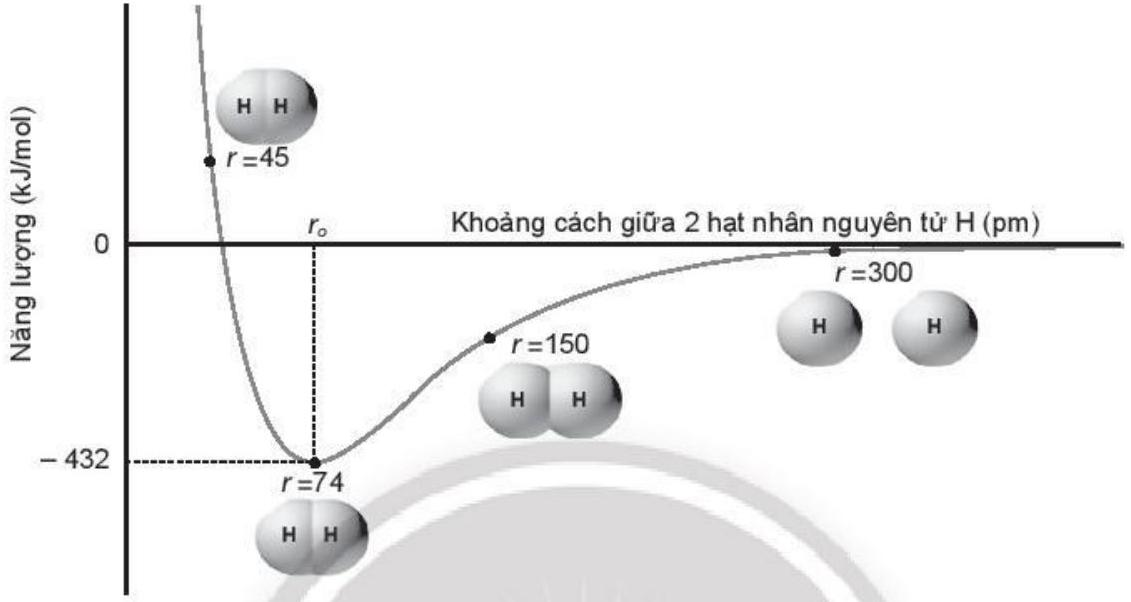
\includegraphics[max width=\textwidth, center]{2025_10_23_883c4b146e2332109fcdg-32(5)}

Cho biết năng lượng liên kết của phân tử hydrogen $\left(\mathrm{H}_{2}\right)$ và độ dài liên kết $\mathrm{H}-\mathrm{H}$ là bao nhiêu? Giải thích.\\
10.23. Sodium chloride tan được trong nước hay trong dầu hoả? Giải thích.\\
10.24. Vì sao benzene $\left(\mathrm{C}_{6} \mathrm{H}_{6}\right)$ không tan trong nước nhưng tan tốt trong các dung môi hữu cơ như tetrachloromethane $\left(\mathrm{CCl}_{4}\right)$, hexane $\left(\mathrm{C}_{6} \mathrm{H}_{14}\right), \ldots$ ?\\
10.25*. Biết phân tử $\mathrm{BF}_{3}$ có cấu trúc phẳng, phân tử $\mathrm{CCl}_{4}$ có cấu trúc hình tứ diện đều. Hãy cho biết có bao nhiêu phân tử phân cực và không phân cực trong hình dưới đây? Giải thích.\\
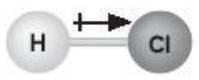
\includegraphics[max width=\textwidth, center]{2025_10_23_883c4b146e2332109fcdg-32(1)}\\
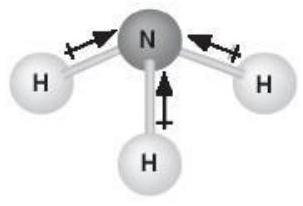
\includegraphics[max width=\textwidth, center]{2025_10_23_883c4b146e2332109fcdg-32(4)}\\
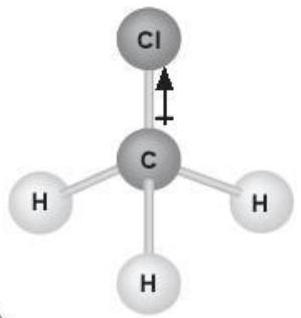
\includegraphics[max width=\textwidth, center]{2025_10_23_883c4b146e2332109fcdg-32(3)}\\
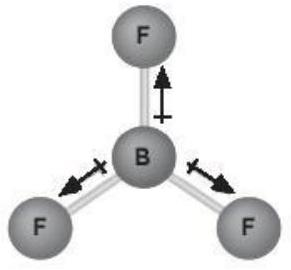
\includegraphics[max width=\textwidth, center]{2025_10_23_883c4b146e2332109fcdg-32}\\
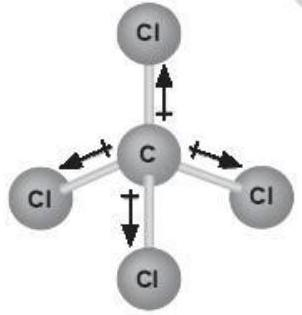
\includegraphics[max width=\textwidth, center]{2025_10_23_883c4b146e2332109fcdg-32(2)}\\
10.26*.\\
a) Ở $25^{\circ} \mathrm{C}$ và $0,99 \mathrm{~atm}$, khả năng tan của carbon dioxide ( $\mathrm{CO}_{2}$ ) trong nước là $1,45 \mathrm{gam} / \mathrm{L}$, kém hơn nhiều so với sulfur dioxide $\left(\mathrm{SO}_{2}\right)$ là 94 gam $/ \mathrm{L}$. Giải thích nguyên nhân sự khác biệt.\\
b) Nhận xét độ tan của carbon dioxide trong nước theo nhiệt độ dựa trên đồ thị sau:\\
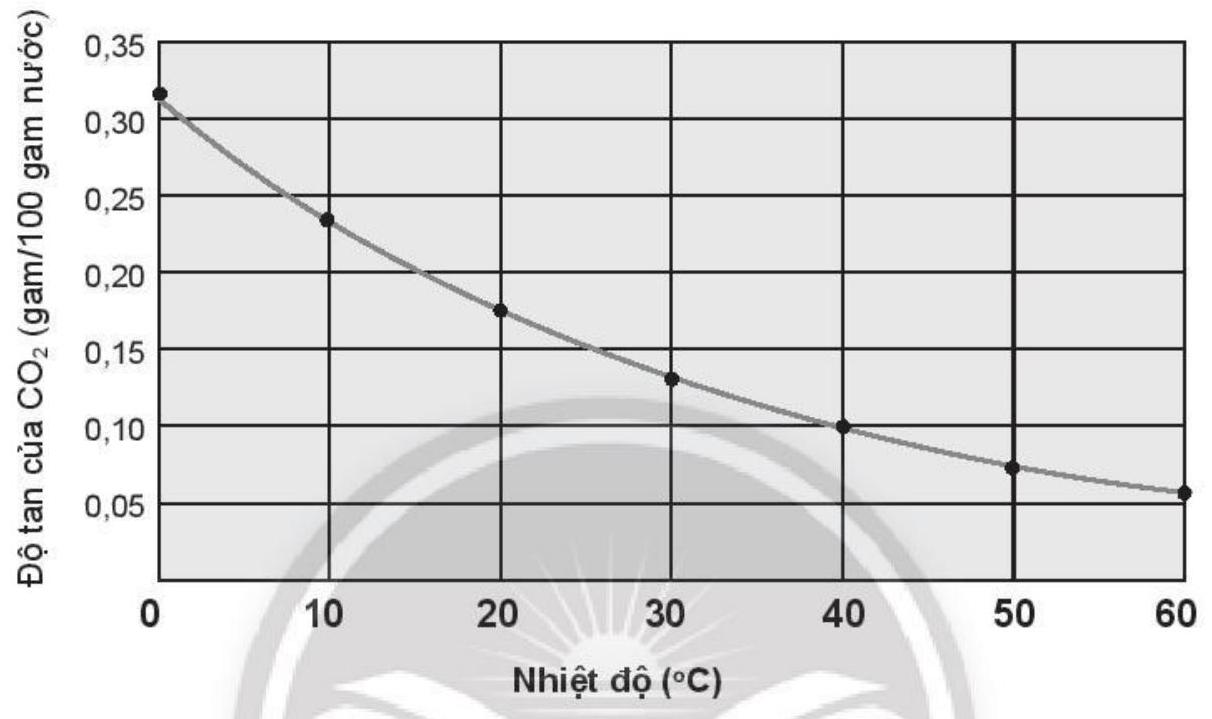
\includegraphics[max width=\textwidth, center]{2025_10_23_883c4b146e2332109fcdg-33}\\
c) Nước giải khát có gas là gi? Vì sao người ta thường ướp lạnh các loại nước giải khát có gas trước khi sử dụng?\\
d) Vì sao trong những ngày hè nóng bức, cá thường phải ngoi lên mặt nước để thở, trong khi vào mùa lạnh, điều này không xảy ra?

\section*{Bai \\
 11}
\section*{LIÊN KẾT HYDROGEN VÀ TƯƠNG TÁC VAN DER WAALS}
11.1. Hợp chất nào sau đây tạo được liên kết hydrogen liên phân tử?\\
A. $\mathrm{H}_{2} \mathrm{~S}$.\\
B. $\mathrm{PH}_{3}$.\\
C. HI.\\
D. $\mathrm{CH}_{3} \mathrm{OH}$.\\
11.2. Mặc dù chlorine có độ âm điện là 3,16 xấp xỉ với nitrogen là 3,04 nhưng giữa các phân tử HCl không tạo được liên kết hydrogen với nhau, trong khi giữa các phân tử $\mathrm{NH}_{3}$ tạo được liên kết hydrogen với nhau, nguyên nhân là do\\
A. độ âm điện của chlorine nhỏ hơn của nitrogen.\\
B. phân tử $\mathrm{NH}_{3}$ chứa nhiều nguyên tử hydrogen hơn phân tử HCl .\\
C. tổng số nguyên tử trong phân tử $\mathrm{NH}_{3}$ nhiều hơn so với phân tử HCl .\\
D. kích thước nguyên tử chlorine lớn hơn nguyên tử nitrogen nên mật độ điện tích âm trên chlorine không đủ lớn để hình thành liên kết hydrogen.\\
11.3. Sơ đồ nào sau đây thể hiện đúng liên kết hydrogen giữa 2 phân tử hydrogen fluoride (HF)?\\
A. $\mathrm{H}^{8+}-\mathrm{F}^{8-} \ldots \mathrm{H}^{3+}-\mathrm{F}^{8-}$.\\
B. $\mathrm{H}^{\delta+}-\mathrm{F}^{\delta+} . . \mathrm{H}^{\delta-}-\mathrm{F}^{\delta-}$.\\
C. $\mathrm{H}^{\delta-}-\mathrm{F}^{\delta+} \ldots \mathrm{H}^{\delta-}-\mathrm{F}^{\delta+}$.\\
D. $\mathrm{H}^{\delta+}-\mathrm{F}^{\delta-} \ldots \mathrm{H}^{\delta-}-\mathrm{F}^{\delta+}$.\\
11.4. Điều nào sau đây đúng khi nói về liên kết hydrogen liên phân tử?\\
A. Là lực hút tĩnh điện giữa nguyên tử H (thường trong các liên kết $\mathrm{H}-\mathrm{F}, \mathrm{H}-\mathrm{N}$, $\mathrm{H}-\mathrm{O}$ ở phân tử này) với một trong các nguyên tử có độ âm điện mạnh (thường là $\mathrm{N}, \mathrm{O}, \mathrm{F}$ ) ở một phân tử khác.\\
B. Là lực hút giữa các phân tử khác nhau.\\
C. Là lực hút tĩnh điện giữa các ion trái dấu.\\
D. Là lực hút giữa các nguyên tử trong một hợp chất cộng hoá trị.\\
11.5. Điều nào sau đây đúng khi nói về liên kết hydrogen nội phân tử?\\
A. Là lực hút giữa các proton của nguyên tử này với các electron ở nguyên tử khác.\\
B. Là lực hút tĩnh điện giữa nguyên tử H (thường trong các liên kết $\mathrm{H}-\mathrm{F}, \mathrm{H}-\mathrm{N}$, $\mathrm{H}-\mathrm{O}$ ) ở một phân tử với một trong các nguyên tử có độ âm điện mạnh (thường là $\mathrm{N}, \mathrm{O}, \mathrm{F}$ ) ở ngay chính phân tử đó.\\
C. Là lực hút giữa các ion trái dấu.\\
D. Là lực hút giữa các phân tử có chứa nguyên tử hydrogen.\\
11.6. Tương tác van der Waals xuất hiện là do sự hình thành các lưỡng cực tạm thời cũng như các lưỡng cực cảm ứng. Các lưỡng cực tạm thời xuất hiện là do sự chuyển động của\\
A. các nguyên tử trong phân tử.\\
B. các electron trong phân tử.\\
C. các proton trong hạt nhân.\\
D. các neutron và proton trong hạt nhân.\\
11.7. Trong các khí hiếm sau, khí hiếm có nhiệt độ sôi cao nhất là\\
A. Ne.\\
B. Xe .\\
C. Ar.\\
D. Kr.\\
11.8. Biểu diễn liên kết hydrogen giữa các phân tử sau:\\
a) methanol $\left(\mathrm{CH}_{3} \mathrm{OH}\right)$ và nước.\\
b) ethylene glycol $\left(\mathrm{HOCH}_{2} \mathrm{CH}_{2} \mathrm{OH}\right)$ và nước.

Từ đó nhận xét tính tan của methanol và ethylene glycol trong nước.\\
11.9. Ethylene glycol $\left(\mathrm{HOCH}_{2} \mathrm{CH}_{2} \mathrm{OH}\right)$ là một chất chống đông trong công nghiệp ô tô, hàng không do có khả năng can thiệp vào liên kết hydrogen của nước, làm các phân tử nước khó liên kết hơn, khiến nước khó đóng băng hơn. Biểu diễn liên kết hydrogen liên phân tử và nội phân tử trong ethylene glycol.\\
11.10. Hãy so sánh tương tác van der Waals với liên kết ion.\\
11.11. Thiết bị chụp cộng hưởng từ hạt nhân (NMR) sử dụng nitrogen lỏng để làm mát nam châm siêu dẫn. Nitrogen lỏng sôi ở $^{\prime} 195,8^{\circ} \mathrm{C}$. Dự đoán nhiệt độ sôi của oxygen lỏng sẽ cao hay thấp hơn so với nitrogen lỏng? Giải thích.\\
11.12. Giải thích vì sao các tương tác van der Waals giữa các phân tử có kích thước lớn lại mạnh hơn so với các phân tử có kích thước nhỏ.\\
11.13*. Giải thích tại sao ở điều kiện thường, các nguyên tố trong nhóm halogen như fluorine và chlorine ở trạng thái khí, còn bromine ở trạng thái lỏng và iodine ở trạng thái rắn.\\
11.14*. Nhiệt độ sôi của các hợp chất với hydrogen của các nguyên tố nhóm VA, VIA và VIIA được biểu diễn qua đồ thị sau:\\
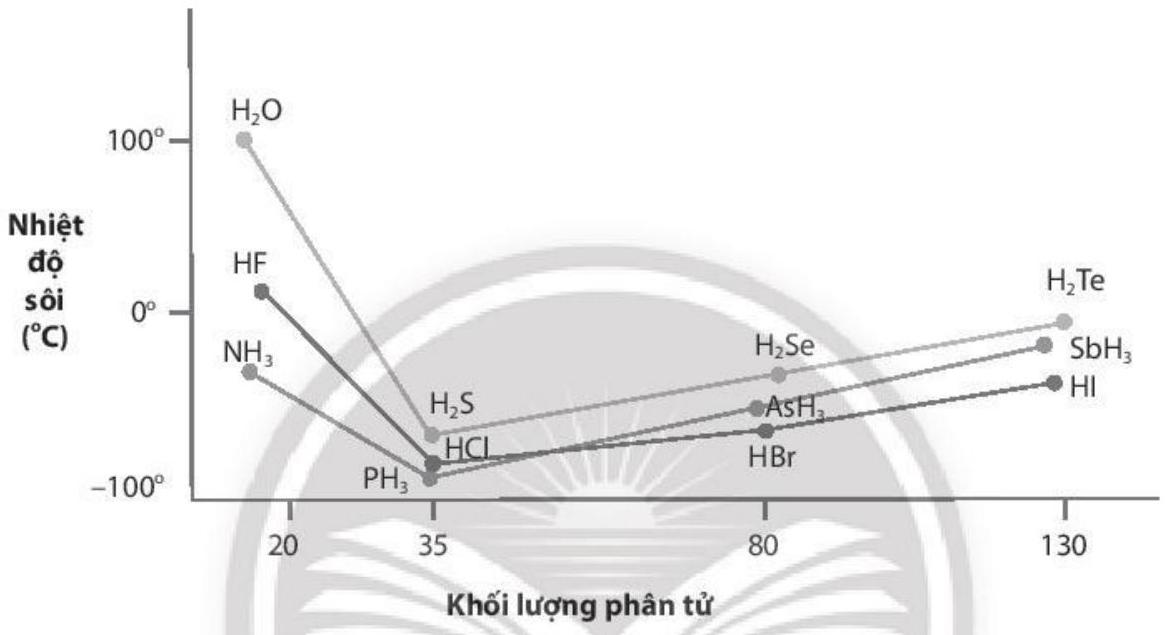
\includegraphics[max width=\textwidth, center]{2025_10_23_883c4b146e2332109fcdg-36}\\
a) Giải thích nhiệt độ sôi cao bất thường của các hợp chất với hydrogen của các nguyên tố đầu tiên trong mỗi nhóm.\\
b) Nhận xét nhiệt độ sôi của các hợp chất với hydrogen của các nguyên tố còn lại ở mỗi nhóm và giải thích nguyên nhân sự biến đổi nhiệt độ sôi của chúng.\\
11.15*. So sánh nhiệt độ nóng chảy và nhiệt độ sôi của pentane ( $\mathrm{CH}_{3} \mathrm{CH}_{2} \mathrm{CH}_{2} \mathrm{CH}_{2} \mathrm{CH}_{3}$ ) và neopentane $\left(\left(\mathrm{CH}_{3}\right)_{4} \mathrm{C}\right)$. Giải thích nguyên nhân sự khác biệt trên.\\
11.16*. Giải thích vì sao tetrachloromethane ( $\mathrm{CCl}_{4}$ ) tuy là phân tử không cực nhưng có nhiệt độ sôi cao hơn trichloromethane $\left(\mathrm{CHCl}_{3}\right)$ là phân tử có cực.

\section*{ÔN TẬP CHƯONG 3}
OT3.1. Ion nào sau đây có cấu hình electron của khí hiếm helium?\\
A. $\mathrm{Mg}^{2+}$.\\
B. $\mathrm{O}^{2-}$.\\
C. $\mathrm{Na}^{+}$.\\
D. $\mathrm{Li}^{+}$.

OT3.2. Trong sự hình thành phân tử lithium fluoride (LiF), ion lithium và ion fluoride đã lần lượt đạt được cấu hình electron bền của các khí hiếm nào?\\
A. Helium và neon.\\
B. Helium và argon.\\
C. Neon và argon.\\
D. Cùng là neon.

OT3.3. Không cần sử dụng hiệu độ âm điện, có bao nhiêu phân tử trong số các phân tử sau có liên kết ion $\mathrm{BaCl}_{2}, \mathrm{CS}_{2}, \mathrm{Na}_{2} \mathrm{O}$ và HI ?\\
A. 3 .\\
B. 2 .\\
C. 4.\\
D. 1.

OT3.4. Tồng số các phân tử có cực trong số các phân tử sau: $\mathrm{Cl}_{2}, \mathrm{O}_{2}, \mathrm{CCl}_{4}, \mathrm{CO}_{2}$ và $\mathrm{SO}_{2}$ là bao nhiêu?\\
A. 1 .\\
B. 2 .\\
C. 4 .\\
D. 3 .

OT3.5. Phân tử sodium fluoride ( NaF ) và magnesium oxide ( MgO ) có cùng 20 electron và khoảng cách giữa các hạt nhân là tương tự nhau ( 235 pm và 215 pm ). Giải thích tại sao nhiệt độ nóng chảy của NaF và MgO lại chênh lệch nhiều $\left(992^{\circ} \mathrm{C}\right.$ so với $2642^{\circ} \mathrm{C}$ ).

OT3.6. Lithium fluoride (LiF) và sodium chloride ( NaCl ) đều là các hợp chất ion. Dự đoán nhiệt độ sôi và nhiệt độ nóng chảy của chất nào cao hơn. Giải thích.

OT3.7. Sodium peroxide $\left(\mathrm{Na}_{2} \mathrm{O}_{2}\right)$ là một chất rắn màu vàng, thu được khi đốt sodium trong khí oxygen dư. Sodium peroxide được dùng để tẩy trắng gỗ, bột giấy, ... Nêu rõ bản chất hoá học giữa các nguyên tử (hoặc nhóm nguyên tử) trong phân tử $\mathrm{Na}_{2} \mathrm{O}_{2}$.

OT3.8. Liên kết hydrogen có phải là sự xen phủ giữa các orbital? Giải thích và cho ví dụ minh hoạ.

OT3.9. Năng lượng liên kết và độ dài liên kết của $\mathrm{C}-\mathrm{C}, \mathrm{C}=\mathrm{C}$ và $\mathrm{C} \equiv \mathrm{C}$ trong các phân tử $\mathrm{C}_{2} \mathrm{H}_{6}, \mathrm{C}_{2} \mathrm{H}_{4}$ và $\mathrm{C}_{2} \mathrm{H}_{2}$ được cho bởi bảng sau:

\begin{center}
\begin{tabular}{|l|l|l|l|}
\hline
Liên kết & $\mathrm{C}-\mathrm{C}$ trong $\mathrm{C}_{2} \mathrm{H}_{6}$ & $\mathrm{C}=\mathrm{C}$ trong $\mathrm{C}_{2} \mathrm{H}_{4}$ & $\mathbf{C \equiv C}$ trong $\mathbf{C}_{\mathbf{2}} \mathbf{H}_{\mathbf{2}}$ \\
\hline
Năng lượng liên kết ( $\mathrm{kJ} / \mathrm{mol}$ ) & 347 & 614 & 839 \\
\hline
Độ dài liên kết (nm) & 0,154 & 0,134 & 0,121 \\
\hline
\end{tabular}
\end{center}

a) Nêu mối quan hệ giữa chiều dài liên kết và năng lượng liên kết giữa các nguyên tử carbon trong các hydrocarbon đã cho.\\
b) Giải thích vì sao giá trị năng lượng liên kết tăng theo thứ tự $\mathrm{C}-\mathrm{C}, \mathrm{C}=\mathrm{C}, \mathrm{C} \equiv \mathrm{C}$.

OT3.10. Ethane $\left(\mathrm{C}_{2} \mathrm{H}_{6}\right)$ và fluoromethane $\left(\mathrm{CH}_{3} \mathrm{~F}\right)$ có kích thước tương đương nhau và đều có 18 electron. Như vậy khả năng hình thành các lưỡng cực tạm thời và lưỡng cực cảm ứng ở cả hai phân tử là như nhau dẫn đến nhiệt độ sôi của chúng phải tương tự nhau. Tuy nhiên, $\mathrm{C}_{2} \mathrm{H}_{6}$ có nhiệt độ sôi là $-89,0^{\circ} \mathrm{C}$ thấp hơn so với $\mathrm{CH}_{3} \mathrm{~F}$ là $-78,3^{\circ} \mathrm{C}$. Giải thích.

\section*{Chưong 4. PHÁN ÚNG OXI HOÁ - KHỦ}
\section*{Baii \\
 12 \\
 PHẢN ÚNG OXI HOÁ - KHỦ VÀ ÚNG DỤNG TRONG CUỘC SỐNG}
12.1. Số oxi hoá của nguyên tử $S$ trong hợp chất $S O_{2}$ là\\
A. +2 .\\
B. +4 .\\
C. +6 .\\
D. -1 .\\
12.2. Dấu hiệu để nhận ra phản ứng là phản ứng oxi hoá - khử dựa trên sự thay đổi đại lượng nào sau đây của nguyên tử?\\
A. Số mol.\\
B. Số oxi hoá.\\
C. Số khối.\\
D. Số proton.

Calcium chloride dùng trong điện phân để sản xuất calcium kim loại và điều chế các hợp kim của calcium. Với tính chất hút ẩm lớn, calcium chloride được dùng làm tác nhân sấy khí và chấtlỏng. Do nhiệt độ đông đặc thấp nên dung dịch calcium(II) chloride được dùng làm chất tải lạnh trong các hệthốnglạnh, ... Ngoài ra, calcium chloride còn được làm chất keo tụ trong hoá dược và dược phẩm hay trong công việc khoan dầu khí.

\begin{figure}[h]
\begin{center}
  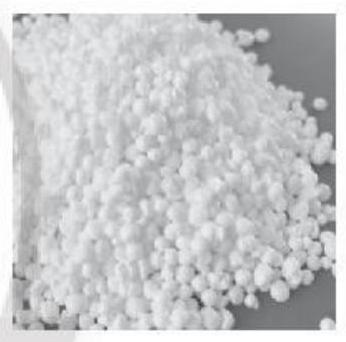
\includegraphics[width=\textwidth]{2025_10_23_883c4b146e2332109fcdg-39}
\captionsetup{labelformat=empty}
\caption{Calcium chloride}
\end{center}
\end{figure}

Dựa vào thông tin trên, hãy trả lời các câu hỏi 12.3. và 12.4.\\
12.3. Trong phản ứng tạo thành calcium(II) chloride từ đơn chất: $\mathrm{Ca}+\mathrm{Cl}_{2} \rightarrow \mathrm{CaCl}_{2}$. Kết luận nào sau đây đúng?\\
A. Mỗi nguyên tử calcium nhận 2 e .\\
B. Mỗi nguyên tử chlorine nhận 2 e .\\
C. Mỗi phân tử chlorine nhường 2 e .\\
D. Mỗi nguyên tử calcium nhường 2 e .\\
12.4. Phản ứng nào sau đây có sự thay đổi số oxi hoá của nguyên tố calcium?\\
A. $\mathrm{Ca}(\mathrm{OH})_{2}+\mathrm{CuCl}_{2} \rightarrow \mathrm{Cu}(\mathrm{OH})_{2}+\mathrm{CaCl}_{2}$\\
B. $\mathrm{CaCl}_{2} \xrightarrow{\text { điện phân nóng chảy }} \mathrm{Ca}+\mathrm{Cl}_{2}$\\
C. $3 \mathrm{CaCl}_{2}+2 \mathrm{~K}_{3} \mathrm{PO}_{4} \rightarrow \mathrm{Ca}_{3}\left(\mathrm{PO}_{4}\right)_{2}+6 \mathrm{KCl}$\\
D. $\mathrm{CaO}+2 \mathrm{HCl} \rightarrow \mathrm{CaCl}_{2}+\mathrm{H}_{2} \mathrm{O}$\\
12.5. Cho các phản ứng sau:\\
(a) $\mathrm{Ca}(\mathrm{OH})_{2}+\mathrm{Cl}_{2} \rightarrow \mathrm{CaOCl}_{2}+\mathrm{H}_{2} \mathrm{O}$\\
(b) $2 \mathrm{NO}_{2}+2 \mathrm{NaOH} \rightarrow \mathrm{NaNO}_{3}+\mathrm{NaNO}_{2}+\mathrm{H}_{2} \mathrm{O}$\\
(c) $\mathrm{O}_{3}+2 \mathrm{Ag} \rightarrow \mathrm{Ag}_{2} \mathrm{O}+\mathrm{O}_{2}$\\
(d) $2 \mathrm{H}_{2} \mathrm{~S}+\mathrm{SO}_{2} \rightarrow 3 \mathrm{~S}+2 \mathrm{H}_{2} \mathrm{O}$\\
(e) $4 \mathrm{KClO}_{3} \rightarrow \mathrm{KCl}+3 \mathrm{KClO}_{4}$

Số phản ứng oxi hoá - khử là\\
A. 2 .\\
B. 3.\\
C. 5.\\
D. 4 .\\
12.6. Phương trình phản ứng nào sau đây không thể hiện tính khử của ammonia $\left(\mathrm{NH}_{3}\right)$ ?\\
A. $4 \mathrm{NH}_{3}+5 \mathrm{O}_{2} \xrightarrow{\mathrm{xt}, \mathrm{t}^{\circ}} 4 \mathrm{NO}+6 \mathrm{H}_{2} \mathrm{O}$\\
B. $\mathrm{NH}_{3}+\mathrm{HCl} \rightarrow \mathrm{NH}_{4} \mathrm{Cl}$\\
C. $2 \mathrm{NH}_{3}+3 \mathrm{Cl}_{2} \rightarrow 6 \mathrm{HCl}+\mathrm{N}_{2}$\\
D. $4 \mathrm{NH}_{3}+3 \mathrm{O}_{2} \xrightarrow{\mathrm{t}^{\circ}} 2 \mathrm{~N}_{2}+6 \mathrm{H}_{2} \mathrm{O}$\\
12.7. Trong phản ứng: $3 \mathrm{Cu}+8 \mathrm{HNO}_{3} \rightarrow 3 \mathrm{Cu}\left(\mathrm{NO}_{3}\right)_{2}+2 \mathrm{NO}+4 \mathrm{H}_{2} \mathrm{O}$. Số phân tử nitric acid $\left(\mathrm{HNO}_{3}\right)$ đóng vai trò chất oxi hoá là\\
A. 8 .\\
B. 6 .\\
C. 4.\\
D. 2 .

Trong thiên nhiên manganesium là nguyên tố tương đối phổ biến, đứng thứ ba trong các kim loại chuyển tiếp, chỉ sau Fe và Ti. Các khoáng vật chính của manganesium là hausmanite $\left(\mathrm{Mn}_{3} \mathrm{O}_{4}\right)$, pyrolusite $\left(\mathrm{MnO}_{2}\right)$, braunite $\left(\mathrm{Mn}_{2} \mathrm{O}_{3}\right)$ và manganite $(\mathrm{MnOOH})$. Manganesium tồn tại ở rất nhiều trạng thái oxi hoá khác nhau từ +2 tới +7 .\\
Dựa vào thông tin trên, hãy trả lời các câu hỏi 12.8 đến 12.10.

\begin{figure}[h]
\begin{center}
  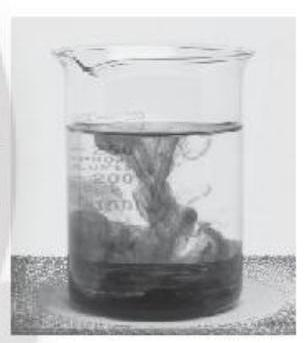
\includegraphics[width=\textwidth]{2025_10_23_883c4b146e2332109fcdg-40}
\captionsetup{labelformat=empty}
\caption{- Dung dịch \$\textbackslash mathrm\{KMnO}\_\{4\}\$\}\end{center}
\end{figure}

12.8. Cho các chất sau: $\mathrm{Mn}, \mathrm{MnO}_{2}, \mathrm{MnCl}_{2}, \mathrm{KMnO}_{4}$ Số oxi hoá của nguyên tố Mn trong các chất lần lượt là\\
A. $2,-2,-4,+8$.\\
B. $0,+4,+2,+7$.\\
C. $0,+4,-2,+7$.\\
D. $0,+2,-4,-7$.\\
12.9. Phản ứng nào sau đây không có sự thay đổi số oxi hoá của nguyên tố Mn?\\
A. $\mathrm{MnO}_{2}+4 \mathrm{HCl} \xrightarrow{\mathrm{t}^{\circ}} \mathrm{MnCl}_{2}+\mathrm{Cl}_{2}+2 \mathrm{H}_{2} \mathrm{O}$\\
B. $\mathrm{Mn}+\mathrm{O}_{2} \rightarrow \mathrm{MnO}_{2}$\\
C. $2 \mathrm{HCl}+\mathrm{MnO} \rightarrow \mathrm{MnCl}_{2}+\mathrm{H}_{2} \mathrm{O}$\\
D. $6 \mathrm{KI}+2 \mathrm{KMnO}_{4}+4 \mathrm{H}_{2} \mathrm{O} \rightarrow 3 \mathrm{I}_{2}+2 \mathrm{MnO}_{2}+8 \mathrm{KOH}$\\
12.10. Sục khí $\mathrm{SO}_{2}$ vào dung dịch $\mathrm{KMnO}_{4}$ (thuốc tím), màu tím nhạt dần rồi mất màu (biết sản phẩm tạo thành là $\mathrm{MnSO}_{4}, \mathrm{H}_{2} \mathrm{SO}_{4}$ và $\mathrm{H}_{2} \mathrm{O}$ ). Nguyên nhân là do\\
A. $\mathrm{SO}_{2}$ đã oxi hoá $\mathrm{KMnO}_{4}$ thành $\mathrm{MnO}_{2}$.\\
B. $\mathrm{SO}_{2}$ đã khử $\mathrm{KMnO}_{4}$ thành $\mathrm{Mn}^{2+}$.\\
C. $\mathrm{KMnO}_{4}$ đã khử $\mathrm{SO}_{2}$ thành $\stackrel{+6}{\mathrm{~S}}$.\\
D. $\mathrm{H}_{2} \mathrm{O}$ đã oxi hoá $\mathrm{KMnO}_{4}$ thành $\mathrm{Mn}^{2+}$.\\
12.11. Xác định số oxi hoá của các nguyên tố trong các chất và ion sau:\\
a) $\mathrm{Fe}, \mathrm{N}_{2}, \mathrm{SO}_{3}, \mathrm{H}_{2} \mathrm{SO}_{4}, \mathrm{CuS} ; \mathrm{Cu}_{2} \mathrm{~S} ; \mathrm{Na}_{2} \mathrm{O}_{2} . \mathrm{H}_{3} \mathrm{AsO}_{4}$.\\
b) $\mathrm{Br}_{2} ; \mathrm{O}_{3} ; \mathrm{HClO}_{3}, \mathrm{KClO}_{4} ; \mathrm{NaClO} ; \mathrm{NH}_{4} \mathrm{NO}_{3} ; \mathrm{N}_{2} \mathrm{O} ; \mathrm{NaNO}_{2}$.\\
c) $\mathrm{Br}^{-}, \mathrm{PO}_{4}^{3-}, \mathrm{MnO}_{4}^{-}, \mathrm{ClO}_{3}^{-}, \mathrm{H}_{2} \mathrm{PO}_{4}^{-}, \mathrm{SO}_{4}^{2-}, \mathrm{NH}_{4}^{+}$.\\
d) $\mathrm{MnO}_{2} ; \mathrm{K}_{2} \mathrm{MnO}_{4} ; \mathrm{K}_{2} \mathrm{Cr}_{2} \mathrm{O}_{7} ; \mathrm{K}_{2} \mathrm{CrO}_{4} ; \mathrm{Cr}_{2}\left(\mathrm{SO}_{4}\right)_{3} ; \mathrm{NaCrO}_{2}$.\\
e) $\mathrm{FeS}_{2} ; \mathrm{FeS} ; \mathrm{FeO} ; \mathrm{Fe}_{2} \mathrm{O}_{3} ; \mathrm{Fe}_{3} \mathrm{O}_{4} ; \mathrm{Fe}_{\mathrm{x}} \mathrm{O}_{\mathrm{y}}$.\\
12.12. Viết các quá trình nhường hay nhận electron của các biến đổi trong các dãy sau:\\
a) $\stackrel{-2}{\mathrm{~S}} \rightarrow \stackrel{0}{\mathrm{~S}} \rightarrow \stackrel{+4}{\mathrm{~S}} \rightarrow \stackrel{+6}{\mathrm{~S}} \rightarrow \stackrel{+4}{\mathrm{~S}}$\\
b) $\stackrel{-3}{\mathrm{~N}} \rightarrow \stackrel{0}{\mathrm{~N}} \rightarrow \stackrel{+2}{\mathrm{~N}} \rightarrow \stackrel{+4}{\mathrm{~N}} \rightarrow \stackrel{+5}{\mathrm{~N}} \rightarrow \stackrel{+2}{\mathrm{~N}}$\\
12.13. Phản ứng nào sau đây là phản ứng oxi hoá - khử? Giải thích.\\
a) $\mathrm{SO}_{3}+\mathrm{H}_{2} \mathrm{O} \rightarrow \mathrm{H}_{2} \mathrm{SO}_{4}$\\
b) $\mathrm{CaCO}_{3}+2 \mathrm{HCl} \rightarrow \mathrm{CaCl}_{2}+\mathrm{CO}_{2} \uparrow+\mathrm{H}_{2} \mathrm{O}$\\
c) $\mathrm{C}+\mathrm{H}_{2} \mathrm{O} \xrightarrow{\mathrm{t}^{\circ}} \mathrm{CO}+\mathrm{H}_{2}$\\
d) $\mathrm{CO}_{2}+\mathrm{Ca}(\mathrm{OH})_{2} \rightarrow \mathrm{CaCO}_{3}+\mathrm{H}_{2} \mathrm{O}$\\
e) $\mathrm{Ca}+2 \mathrm{H}_{2} \mathrm{O} \rightarrow \mathrm{Ca}(\mathrm{OH})_{2}+\mathrm{H}_{2} \uparrow$\\
g) $2 \mathrm{KMnO}_{4} \xrightarrow{\mathrm{t}^{\circ}} \mathrm{K}_{2} \mathrm{MnO}_{4}+\mathrm{MnO}_{2}+\mathrm{O}_{2} \uparrow$\\
12.14. Gỉ sét là quá trình oxi hoá kim loại, mỗi năm phá huỷ khoảng $25 \%$ sắt thép. Gỉ sét được hình thành do kim loại sắt $(\mathrm{Fe})$ trong gang hay thép kết hợp với oxygen khi có mặt nước hoặc không khí ẩm. Trên bề mặt gang hay thép bị gỉ hình thành những lớp xốp và giòn dễ vỡ, thường có màu nâu, nâu đỏ hoặc đỏ. Lớp gỉ này không có tác dụng bảo vệ sắt

\begin{figure}[h]
\begin{center}
  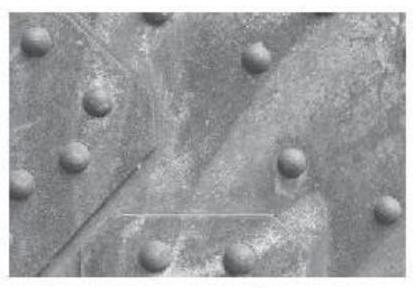
\includegraphics[width=\textwidth]{2025_10_23_883c4b146e2332109fcdg-41}
\captionsetup{labelformat=empty}
\caption{A Gỉ sắt}
\end{center}
\end{figure}

ở phía trong. Sau thời gian dài, bất kì khối sắt nào cũng sẽ bị gỉ hoàn toàn và phân huỷ. Thành phần chính của sắt gỉ gồm $\mathrm{Fe}(\mathrm{OH})_{2}, \mathrm{Fe}_{2} \mathrm{O}_{3} \cdot \mathrm{nH}_{2} \mathrm{O}$.

Một số phản ứng xảy ra trong quá trình gỉ sắt:


\begin{align*}
& \mathrm{Fe}+\mathrm{O}_{2}+\mathrm{H}_{2} \mathrm{O} \rightarrow \mathrm{Fe}(\mathrm{OH})_{2}  \tag{1}\\
& \mathrm{Fe}+\mathrm{O}_{2}+\mathrm{H}_{2} \mathrm{O}+\mathrm{CO}_{2} \rightarrow \mathrm{Fe}\left(\mathrm{HCO}_{3}\right)_{2}  \tag{2}\\
& \mathrm{Fe}\left(\mathrm{HCO}_{3}\right)_{2} \rightarrow \mathrm{Fe}(\mathrm{OH})_{2}+\mathrm{CO}_{2}  \tag{3}\\
& \mathrm{Fe}(\mathrm{OH})_{2}+\mathrm{O}_{2}+\mathrm{H}_{2} \mathrm{O} \rightarrow \mathrm{Fe}_{2} \mathrm{O}_{3} . \mathrm{nH}_{2} \mathrm{O} \tag{4}
\end{align*}


a) Phản ứng nào ở trên là phản ứng oxi hoá - khử?\\
b) Xác định sự thay đổi số oxi hoá của các nguyên tố, nêu rõ chất oxi hoá, chất khử.\\
c) Cân bằng phản ứng trên bằng phương pháp thăng bằng electron.\\
12.15. Rượu gạo là một thức uống có cồn lên men được chưng cất từ gạo theo truyền thống. Rượu gạo được làm từ quá trình lên men tinh bột gạo đã được chuyển thành đường. Vi khuẩn là nguồn gốc của các enzyme chuyển đổi tinh bột thành đường. Nhiệt độ phù hợp để lên men rượu khoảng $20-25^{\circ} \mathrm{C}$.\\
Phản ứng thuỷ phân và phản ứng lên men:\\
(1) $\left(\mathrm{C}_{6} \mathrm{H}_{10} \mathrm{O}_{5}\right)_{n}+n \mathrm{H}_{2} \mathrm{O} \rightarrow n \mathrm{C}_{6} \mathrm{H}_{12} \mathrm{O}_{6}$\\
(2) $\mathrm{C}_{6} \mathrm{H}_{12} \mathrm{O}_{6} \xrightarrow{\mathrm{I}^{\circ} \text {, enzyme }} 2 \mathrm{C}_{2} \mathrm{H}_{5} \mathrm{OH}+2 \mathrm{CO}_{2}$

\begin{figure}[h]
\begin{center}
  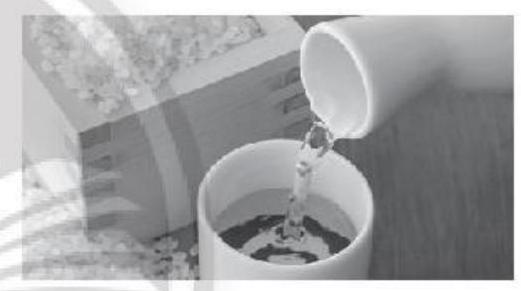
\includegraphics[width=\textwidth]{2025_10_23_883c4b146e2332109fcdg-42}
\captionsetup{labelformat=empty}
\caption{- Rượu nấu từ gạo}
\end{center}
\end{figure}

a) Phản ứng nào ở trên là phản ứng oxi hoá - khử? Giải thích.\\
b) Trong phản ứng oxi hoá - khử, em hãy xác định số oxi hoá của các nguyên tố, nêu rõ chất oxi hoá, chất khử.\\
c) Cân bằng phản ứng oxi hoá - khử trên bằng phương pháp thăng bằng electron.\\
12.16. Cân bằng phản ứng sau bằng phương pháp thăng bằng electron, nêu rõ chất oxi hoá, chất khử trong mỗi trường hợp sau:\\
a) $\mathrm{H}_{2} \mathrm{~S}+\mathrm{SO}_{2} \rightarrow \mathrm{~S}+\mathrm{H}_{2} \mathrm{O}$\\
b) $\mathrm{SO}_{2}+\mathrm{H}_{2} \mathrm{O}+\mathrm{Cl}_{2} \rightarrow \mathrm{H}_{2} \mathrm{SO}_{4}+\mathrm{HCl}$\\
c) $\mathrm{FeS}_{2}+\mathrm{O}_{2} \rightarrow \mathrm{Fe}_{2} \mathrm{O}_{3}+\mathrm{SO}_{2}$\\
d) $\mathrm{C}_{12} \mathrm{H}_{22} \mathrm{O}_{11}+\mathrm{H}_{2} \mathrm{SO}_{4} \rightarrow \mathrm{CO}_{2}+\mathrm{SO}_{2}+\mathrm{H}_{2} \mathrm{O}$\\
12.17*. Cho potassium iodide (KI) tác dụng với potassium permanganate $\left(\mathrm{KMnO}_{4}\right)$ trong dung dịch sulfuric acid $\left(\mathrm{H}_{2} \mathrm{SO}_{4}\right)$, thu được $3,02 \mathrm{~g}$ manganese(II) sulfate $\left(\mathrm{MnSO}_{4}\right), \mathrm{I}_{2}$ và $\mathrm{K}_{2} \mathrm{SO}_{4}$.\\
a) Tính số gam iodine $\left(\mathrm{I}_{2}\right)$ tạo thành.\\
b) Tính khối lượng potassium iodide (KI) đã tham gia phản ứng.\\
12.18*. Hoà tan 14 g Fe trong dung dịch $\mathrm{H}_{2} \mathrm{SO}_{4}$ loãng, dư, thu được dung dịch X . Thêm dung dịch $\mathrm{KMnO}_{4} 1 \mathrm{M}$ vào dung dịch X . Biết $\mathrm{KMnO}_{4}$ có thể oxi hoá FeSO ${ }_{4}$ trong môi trường $\mathrm{H}_{2} \mathrm{SO}_{4}$ thành $\mathrm{Fe}_{2}\left(\mathrm{SO}_{4}\right)_{3}$ và bị khử thành $\mathrm{MnSO}_{4}$. Phản ứng xảy ra hoàn toàn. Lập phương trình hoá học cho phản ứng oxi hoá - khử trên. Tính thể tích dung dịch $\mathrm{KMnO}_{4} 1 \mathrm{M}$ đã phản ứng.\\
12.19*. Nitric acid $\left(\mathrm{HNO}_{3}\right)$ là hợp chất vô cơ, trong tự nhiên, được hình thành trong những cơn mưa giông kèm sấm chớp. Nitric acid là một acid độc, ăn mòn và dễ gây cháy, là một trong những tác nhân gây ra mưa acid.\\
Thực hiện thí nghiệm xác định công thức của một oxide của kim loại sắt bằng nitric acid đặc nóng, thu được 2,479 lít (đkc) khí màu nâu là nitrogen dioxide. Phần dung dịch đem cô cạn thì được $72,6 \mathrm{~g} \mathrm{Fe}\left(\mathrm{NO}_{3}\right)_{3}$. Giả sử phản ứng không tạo thành các sản phẩm khác (biết 1 mol khí chiếm 24,79 lít đo ở đkc $25^{\circ} \mathrm{C}, 1$ bar).\\
a) Viết phản ứng và cân bằng bằng phương pháp thăng bằng electron.\\
b) Xác định công thức của iron oxide.\\
12.20*. Có nhiều vụ tai nạn giao thông xảy ra do người lái xe uống rượu. Theo luật định, hàm lượng ethanol trong máu người lái xe không vượt quá $0,02 \%$ theo khối lượng. Để xác định hàm lượng ethanol trong máu của người lái xe cần chuẩn độ ethanol bằng $\mathrm{K}_{2} \mathrm{Cr}_{2} \mathrm{O}_{7}$ trong môi trường acid. Khi đó $\mathrm{Cr}^{+6}$ bị khử thành $\mathrm{Cr}^{+3}$, ethanol $\left(\mathrm{C}_{2} \mathrm{H}_{5} \mathrm{OH}\right)$ bị oxi hoá thành acetaldehyde $\left(\mathrm{CH}_{3} \mathrm{CHO}\right)$.\\
a) Hãy viết phương trình hoá học của phản ứng.\\
b) Khi chuẩn độ 25 g huyết tương máu của một lái xe cần dùng 20 mL dung dịch $\mathrm{K}_{2} \mathrm{Cr}_{2} \mathrm{O}_{7} 0,01 \mathrm{M}$. Người lái xe đó có vi phạm luật hay không? Tại sao? Giả sử rằng trong thí nghiệm trên chỉ có ethanol tác dụng với $\mathrm{K}_{2} \mathrm{Cr}_{2} \mathrm{O}_{7}$.

\section*{ÔN TẬP CHƯONG 4}
OT4.1. Sản xuất gang trong công nghiệp bằng cách sử dụng khí CO khử $\mathrm{Fe}_{2} \mathrm{O}_{3}$ ở nhiệt độ cao theo phản ứng sau:

$$
\mathrm{Fe}_{2} \mathrm{O}_{3}+3 \mathrm{CO} \xrightarrow{\mathrm{t}^{\circ}} 2 \mathrm{Fe}+3 \mathrm{CO}_{2}
$$

Trong phản ứng trên chất đóng vai trò chất khử là\\
A. $\mathrm{Fe}_{2} \mathrm{O}_{3}$.\\
B. CO .\\
C. Fe.\\
D. $\mathrm{CO}_{2}$.

OT4.2. Cho các phân tử có công thức cấu tạo sau:\\
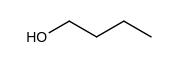
\includegraphics{smile-0fc5a791cf282450699c8f3470338a3e1e399b14}\\
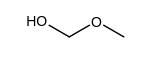
\includegraphics{smile-958568a22d3b651308cf7b8bb03c2c0fb39e5865}\\
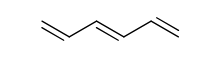
\includegraphics{smile-769e7e0de1da77c25bd6b32b601a7db81ef32a22}

Số oxi hoá trung bình của nguyên tử C trong các phân tử trên lần lượt là\\
A. $-3,-2,-2$.\\
B. $-3,-3,-2$.\\
C. $-2,-2,-2$.\\
D. $-3,-2,-3$.

OT4.3. Thực hiện các phản ứng sau:\\
(a) $\mathrm{Ca}(\mathrm{OH})_{2}+\mathrm{Cl}_{2} \longrightarrow \mathrm{CaOCl}_{2}+\mathrm{H}_{2} \mathrm{O}$\\
(b) $3 \mathrm{Cl}_{2}+6 \mathrm{KOH} \xrightarrow{\mathrm{t}^{\circ}} 5 \mathrm{KCl}+\mathrm{KClO}_{3}+3 \mathrm{H}_{2} \mathrm{O}$\\
(c) $\mathrm{Cl}_{2}+2 \mathrm{FeCl}_{2} \longrightarrow 2 \mathrm{FeCl}_{3}$\\
(d) $2 \mathrm{KClO}_{3} \xrightarrow{\mathrm{t}^{\circ}} 2 \mathrm{KCl}+3 \mathrm{O}_{2}$

Số phản ứng chlorine đóng vai trò chất oxi hoá là\\
A. 1 .\\
B. 2 .\\
C. 3.\\
D. 4 .

OT4.4. Bromine vừa là chất oxi hoá, vừa là chất khử trong phản ứng nào sau đây?\\
A. $3 \mathrm{Br}_{2}+6 \mathrm{NaOH} \longrightarrow 5 \mathrm{NaBr}+\mathrm{NaBrO}_{3}+3 \mathrm{H}_{2} \mathrm{O}$\\
B. $\mathrm{Br}_{2}+\mathrm{H}_{2} \xrightarrow{\mathrm{t}^{\circ}} 2 \mathrm{HBr}$\\
C. $3 \mathrm{Br}_{2}+2 \mathrm{Al} \rightarrow 2 \mathrm{AlBr}_{3}$\\
D. $\mathrm{Br}_{2}+2 \mathrm{KI} \rightarrow \mathrm{I}_{2}+2 \mathrm{KBr}$

OT4.5. Nguyên tử sulfur chỉ thể hiện tính khử (trong điều kiện phản ứng phù hợp) trong hợp chất nào sau đây?\\
A. $\mathrm{SO}_{2}$.\\
B. $\mathrm{H}_{2} \mathrm{SO}_{4}$.\\
C. $\mathrm{H}_{2} \mathrm{~S}$.\\
D. $\mathrm{Na}_{2} \mathrm{SO}_{3}$.

OT4.6. Tính số oxi hoá các nguyên tố có đánh dấu *:\\
a) $\mathrm{Na}_{2} \stackrel{*}{\mathrm{CrO}}, \mathrm{Ca}_{3}\left(\stackrel{*}{\mathrm{PO}_{4}}\right)_{2}, \mathrm{CaSiO}_{3}, \mathrm{NaCrO}, \mathrm{FeS}_{2}$.\\
b) $\stackrel{*}{\mathrm{~N}} \mathrm{H}_{4}^{+}, \stackrel{*}{\mathrm{Cr}_{2}} \mathrm{O}_{7}^{2-}, \stackrel{*}{\mathrm{MnO}_{4}^{2-}}, \stackrel{*}{\mathrm{NO}_{2}^{-}}$.

OT4.7. Chất được gạch chân trong các phương trình hoá học sau đây là chất oxi hoá hay chất khử, nêu lí do.\\
a) $\underline{\mathrm{Br}}_{2}+2 \mathrm{KI} \rightarrow \mathrm{I}_{2}+2 \mathrm{KBr}$\\
b) $3 \mathrm{Zn}+8 \mathrm{HNO}_{3} \rightarrow 3 \mathrm{Zn}\left(\mathrm{NO}_{3}\right)_{2}+3 \mathrm{NO}+4 \mathrm{H}_{2} \mathrm{O}$\\
c) $\underline{\mathrm{K}}_{2} \underline{\mathrm{Cr}}_{2} \underline{\mathrm{O}}_{7}+14 \mathrm{HCl} \rightarrow 2 \mathrm{CrCl}_{3}+2 \mathrm{KCl}+3 \mathrm{Cl}_{2}+7 \mathrm{H}_{2} \mathrm{O}$

OT4.8. Dẫn ra hai phản ứng, trong đó có một phản ứng oxi hoá - khử và một không phải phản ứng oxi hoá- khử.\\
OT4.9. Dưới tác dụng của các chất xúc tác, glucose tạo thành các sản phẩm khác nhau.

\begin{itemize}
  \item Lên men tạo thành ethanol:
\end{itemize}


\begin{equation*}
\underset{\text { (glucose) }}{\mathrm{C}_{6} \mathrm{H}_{12} \mathrm{O}_{6}} \xrightarrow[\text { (ethanol) }]{\text { enzyme }} \underset{\text { (eth }}{\mathrm{C}_{2} \mathrm{H}_{5} \mathrm{OH}}+\mathrm{CO}_{2} \tag{1}
\end{equation*}


\begin{itemize}
  \item Ethanol lên men thành acetic acid:
\end{itemize}


\begin{equation*}
\mathrm{CH}_{3}-\mathrm{CH}_{2}-\mathrm{OH}+\mathrm{O}_{2} \xrightarrow{\text { enzyme }} \underset{\text { (acetic acid) }}{\mathrm{CH}_{3}-\mathrm{COOH}+\mathrm{H}_{2} \mathrm{O}} \tag{2}
\end{equation*}


a) Cho biết vai trò của các chất trong các phản ứng (1) và (2).\\
b) Tính lượng glucose cần dùng để thu được 1 lít acetic acid 1 M . Giả sử hiệu suất của cả quá trình là $50 \%$.\\
OT4.10. Ion $\mathrm{Ca}^{2+}$ cần thiết cho máu của người hoạt động bình thường. Nồng độ ion calcium không bình thường là dấu hiệu của bệnh. Để xác định nồng độ ion calcium, người ta lấy mẫu máu, sau đó kết tủa ion calcium dưới dạng calcium oxalate $\left(\mathrm{CaC}_{2} \mathrm{O}_{4}\right)$ rồi cho calcium oxalate tác dụng với dung dịch potassium permanganate trong môi trường acid theo phản ứng sau:

$$
\mathrm{KMnO}_{4}+\mathrm{CaC}_{2} \mathrm{O}_{4}+\mathrm{H}_{2} \mathrm{SO}_{4} \rightarrow \mathrm{CaSO}_{4}+\mathrm{K}_{2} \mathrm{SO}_{4}+\mathrm{MnSO}_{4}+\mathrm{CO}_{2} \uparrow+\mathrm{H}_{2} \mathrm{O}
$$

a) Cân bằng phương trình phản ứng.\\
b) Giả sử calcium oxalate kết tủa từ 1 mL máu một người tác dụng vừa hết với $2,05 \mathrm{~mL}$ dung dịch potassium permanganate $\left(\mathrm{KMnO}_{4}\right) 4,88.10^{-4} \mathrm{M}$. Xác định nồng độ ion calcium trong máu người đó bằng đơn vị $\mathrm{mg} \mathrm{Ca}^{2+} / 100 \mathrm{~mL}$ máu.\\
OT4.11. Hỗn hợp ammonium perchlorate $\left(\mathrm{NH}_{4} \mathrm{ClO}_{4}\right)$ và bột nhôm là nhiên liệu rắn của tàu vũ trụ con thoi theo phản ứng sau:

$$
\mathrm{NH}_{4} \mathrm{ClO}_{4} \rightarrow \mathrm{~N}_{2} \uparrow+\mathrm{Cl}_{2} \uparrow+\mathrm{O}_{2} \uparrow+\mathrm{H}_{2} \mathrm{O}
$$

Mỗi một lần phóng tàu con thoi tiêu tốn 750 tấn ammonium perchlorate. Giả sử tất cả oxygen sinh ra tác dụng với bột nhôm, hãy tính khối lượng nhôm phản ứng với oxygen và khối lượng aluminium oxide sinh ra.\\
OT4.12. Cho $30,3 \mathrm{~g}$ hổn hợp Al và Zn tác dụng vừa đủ với 11,15 lít $\mathrm{O}_{2}$ (đkc), thu được hổn hợp các oxide. Viết các phương trình phản ứng xảy ra và tính khối lượng các oxide tạo thành.

OT4.13. Sodium peroxide $\left(\mathrm{Na}_{2} \mathrm{O}_{2}\right)$, potassium superoxide $\left(\mathrm{KO}_{2}\right)$ là những chất oxi hoá mạnh, dễ dàng hấp thụ khí carbon dioxide và giải phóng khí oxygen. Do đó, chúng được sử dụng trong bình lặn hoặc tàu ngầm để hấp thụ khí carbon dioxide và cung cấp khí oxygen cho con người trong hô hấp theo các phản ứng sau:\\
$\mathrm{Na}_{2} \mathrm{O}_{2}+\mathrm{CO}_{2} \rightarrow \mathrm{Na}_{2} \mathrm{CO}_{3}+\mathrm{O}_{2} \uparrow$\\
$\mathrm{KO}_{2}+\mathrm{CO}_{2} \rightarrow \mathrm{~K}_{2} \mathrm{CO}_{3}+\mathrm{O}_{2} \uparrow$\\
a) Cân bằng các phản ứng biết rằng nguyên tử oxygen trong $\mathrm{Na}_{2} \mathrm{O}_{2}, \mathrm{KO}_{2}$ là nguyên tố tự oxi hoá - khử.

\begin{figure}[h]
\begin{center}
  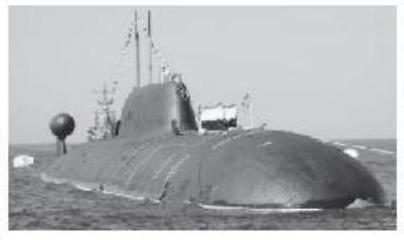
\includegraphics[width=\textwidth]{2025_10_23_883c4b146e2332109fcdg-46(1)}
\captionsetup{labelformat=empty}
\caption{A Tàu ngầm}
\end{center}
\end{figure}

\begin{figure}[h]
\begin{center}
  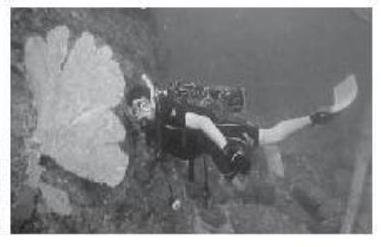
\includegraphics[width=\textwidth]{2025_10_23_883c4b146e2332109fcdg-46}
\captionsetup{labelformat=empty}
\caption{A Thợ lặn dùng bình dưỡng khí}
\end{center}
\end{figure}

b) Theo nghiên cứu, khi hô hấp, thể tích khí carbon dioxide một người thải ra xấp xỉ thể tích khí oxygen hít vào. Cần trộn $\mathrm{Na}_{2} \mathrm{O}_{2}$ và $\mathrm{KO}_{2}$ theo tỉ lệ số mol như thế nào để thể tích khí carbon dioxide hấp thụ bằng thể tích khi oxygen sinh ra?\\
OT4. 14. Copper(II) sulfate được sử dụng làm nguyên liệu trong phân bón, làm thuốc kháng nấm. Ngoài ra,còn dùng để diệt rêu - tảo trong bể bơi, ... Copper(II) sulfate được sản xuất chủ yếu sử dụng từ nguồn nguyên liệu tái chế. Phế liệu được tinh chế cùng kim loại nóng chảy được đổ vào nước để tạo thành những mảnh xốp. Hổn hợp này được hoà tan trong dung dịch sulfuric acid loãng trong không khí theo phương trình: $\mathrm{Cu}+\mathrm{O}_{2}+\mathrm{H}_{2} \mathrm{SO}_{4} \rightarrow \mathrm{CuSO}_{4}+\mathrm{H}_{2} \mathrm{O}$ (1\\
Ngoài ra, copper(II) sulfate còn được điều chế bằng cách cho đồng phế liệu tác dụng với dung dịch sunfuric acid đặc, nóng: $\mathrm{Cu}+\mathrm{H}_{2} \mathrm{SO}_{4} \rightarrow \mathrm{CuSO}_{4}+\mathrm{SO}_{2}+\mathrm{H}_{2} \mathrm{O}$ (2).\\

\includegraphics[max width=\textwidth, center]{2025_10_23_883c4b146e2332109fcdg-46(2)}

\section*{- Tinh thể muối copper(II) sulfate}
a) Cân bằng 2 phản ứng trên theo phương pháp thăng bằng electron.\\
b) Trong hai cách trên, cách nào ít làm ô nhiễm môi trường hơn?

OT4.15. Cho $1,12 \mathrm{~g}$ kim loại X tác dụng với dung dịch sulfuric acid đặc, nóng, dư thu được 0,7437 lít khí $\mathrm{SO}_{2}$ (đkc) và muối $\mathrm{X}_{2}\left(\mathrm{SO}_{4}\right)_{3}$.\\
a) Viết phản ứng và cân bằng phương trình hoá học theo phương pháp thăng bằng electron.\\
b) Xác định kim loại $X$.

\section*{Chuong 5. NĂNG LUỌNG HOÁ HỌC}
\section*{Bai \\
 13}
\section*{ENTHALPY TẠO THÀNH VÀ BIẾN THIÊN ENTHALPY CỦA PHẢN ỨNG HOÁ HỌC}
13.1. Cho phương trình nhiệt hoá học của phản ứng:\\
$2 \mathrm{H}_{2}(g)+\mathrm{O}_{2}(g) \rightarrow 2 \mathrm{H}_{2} \mathrm{O}(l)$\\
$\Delta_{\mathrm{r}} \mathrm{H}_{298}^{\circ}=-571,68 \mathrm{~kJ}$\\
Phản ứng trên là phản ứng\\
A. thu nhiệt.\\
B. toả nhiệt.\\
C. không có sự thay đồi năng lượng.\\
D. có sự hấp thụ nhiệt lượng từ môi trường xung quanh.\\
13.2. Cho phương trình nhiệt hoá học của phản ứng:\\
$\mathrm{N}_{2}(g)+\mathrm{O}_{2}(g)$ $\_\_\_\_$ $\xrightarrow{\mathrm{t}^{\circ}} 2 \mathrm{NO}(g)$\\
$\Delta_{\mathrm{r}} \mathrm{H}_{298}^{\circ}=+179,20 \mathrm{~kJ}$\\
Phản ứng trên là phản ứng\\
A. thu nhiệt.\\
B. không có sự thay đổi năng lượng.\\
C. toả nhiệt.\\
D. có sự giải phóng nhiệt lượng ra môi trường.\\
13.3. Dựa vào phương trình nhiệt hoá học của phản ứng sau:\\
$\mathrm{CO}_{2}(g) \rightarrow \mathrm{CO}(g)+\frac{1}{2} \mathrm{O}_{2}(g)$

$$
\Delta_{\mathrm{r}} \mathrm{H}_{298}^{\circ}=+280 \mathrm{~kJ}
$$

Giá trị $\Delta_{\mathrm{r}} \mathrm{H}_{298}^{\circ}$ của phản ứng: $2 \mathrm{CO}_{2}(g) \rightarrow 2 \mathrm{CO}(g)+\mathrm{O}_{2}(g)$ là\\
A. +140 kJ .\\
B. -1120 kJ .\\
C. +560 kJ .\\
D. -420 kJ .\\
13.4. Phương trình nhiệt hoá học:\\
$3 \mathrm{H}_{2}(\mathrm{~g})+\mathrm{N}_{2}(\mathrm{~g}) \xrightarrow{\mathrm{t}^{\circ}} 2 \mathrm{NH}_{3}(\mathrm{~g}) \quad \Delta_{\mathrm{r}} \mathrm{H}_{298}^{\circ}=-91,80 \mathrm{~kJ}$\\
Lượng nhiệt toả ra khi dùng $9 \mathrm{~g} \mathrm{H}_{2}(\mathrm{~g})$ để tạo thành $\mathrm{NH}_{3}(\mathrm{~g})$ là\\
A. $-275,40 \mathrm{~kJ}$.\\
B. $-137,70 \mathrm{~kJ}$.\\
C. $-45,90 \mathrm{~kJ}$.\\
D. $-183,60 \mathrm{~kJ}$.\\
13.5. Điều kiện nào sau đây không phải là điều kiện chuẩn?\\
A. Áp suất 1 bar và nhiệt độ $25^{\circ} \mathrm{C}$ hay 298 K .\\
B. Áp suất 1 bar và nhiệt độ 298 K .\\
C. Áp suất 1 bar và nhiệt độ $25^{\circ} \mathrm{C}$.\\
D. Áp suất 1 bar và nhiệt độ 25 K .\\
13.6. Dựa vào phương trình nhiệt hoá học của các phản ứng sau:


\begin{equation*}
\mathrm{CS}_{2}(\mathrm{l})+3 \mathrm{O}_{2}(\mathrm{~g}) \xrightarrow{\mathrm{t}^{\circ}} \mathrm{CO}_{2}(\mathrm{~g})+2 \mathrm{SO}_{2}(\mathrm{~g}) \quad \Delta_{\mathrm{r}} \mathrm{H}_{298}^{\circ}=-1110,21 \mathrm{~kJ} \tag{1}
\end{equation*}



\begin{equation*}
\mathrm{CO}_{2}(g) \rightarrow \mathrm{CO}(g)+\frac{1}{2} \mathrm{O}_{2}(g) \tag{2}
\end{equation*}


$\Delta_{\mathrm{r}} \mathrm{H}_{298}^{\mathrm{o}}=+280,00 \mathrm{~kJ}$


\begin{equation*}
\mathrm{Na}(s)+2 \mathrm{H}_{2} \mathrm{O}(l) \rightarrow \mathrm{NaOH}(a q)+\mathrm{H}_{2}(g) \tag{3}
\end{equation*}


$\Delta_{\mathrm{r}} \mathrm{H}_{298}^{\circ}=-367,50 \mathrm{~kJ}$


\begin{equation*}
\mathrm{ZnSO}_{4}(s) \rightarrow \mathrm{ZnO}(s)+\mathrm{SO}_{3}(g) \tag{4}
\end{equation*}


$\Delta_{\mathrm{r}} \mathrm{H}_{298}^{\circ}=+235,21 \mathrm{~kJ}$

Cặp phản ứng thu nhiệt là:\\
A. (1) và (2).\\
B. (3) và (4).\\
C. (1) và (3).\\
D. (2) và (4).\\
13.7. Dựa vào phương trình nhiệt hoá học của phản ứng sau:

$$
3 \mathrm{Fe}(s)+4 \mathrm{H}_{2} \mathrm{O}(l) \rightarrow \mathrm{Fe}_{3} \mathrm{O}_{4}(s)+4 \mathrm{H}_{2}(g) \quad \Delta_{r} \mathrm{H}_{298}^{\circ}=+26,32 \mathrm{~kJ}
$$

Giá trị $\Delta_{\mathrm{r}} \mathrm{H}_{298}^{\circ}$ của phản ứng: $\mathrm{Fe}_{3} \mathrm{O}_{4}(s)+4 \mathrm{H}_{2}(g) \rightarrow 3 \mathrm{Fe}(s)+4 \mathrm{H}_{2} \mathrm{O}(l)$ là\\
A. $-26,32 \mathrm{~kJ}$.\\
B. $+13,16 \mathrm{~kJ}$.\\
C. $+19,74 \mathrm{~kJ}$.\\
D. $-10,28 \mathrm{~kJ}$.\\
13.8. a) Enthalpy tạo thành của hợp chất là gì?\\
b) Biến thiên enthalpy trong các phản ứng hoá học là gì?\\
c) Enthalpy tạo thành khác với enthalpy tạo thành chuẩn ở điểm nào?\\
d) Tại sao enthalpy tạo thành chuẩn của đơn chất lại bằng không?\\
13.9. Các quá trình sau đây là toả nhiệt hay thu nhiệt?\\
a) Nước hoá rắn.\\
b) Sự tiêu hoá thức ăn.\\
c) Quá trình chạy của con người.\\
d) Khí $\mathrm{CH}_{4}$ đốt ở trong lò.\\
e) Hoà tan KBr vào nước làm cho nước trở nên lạnh.\\
g) Sulfuric acid đặc khi thêm vào nước làm cho nước nóng lên.\\
13.10. Hãy nêu 1 phản ứng toả nhiệt và 1 phản ứng thu nhiệt mà em biết.\\
13.11. Khi đun nóng muối ammonium nitrate bị nhiệt phân theo phương trình:

$$
\mathrm{NH}_{4} \mathrm{NO}_{3} \xrightarrow{t^{\circ}} \mathrm{N}_{2} \mathrm{O}+2 \mathrm{H}_{2} \mathrm{O}
$$

Hãy dự đoán phản ứng trên là toả nhiệt hay thu nhiệt.\\
13.12. Một phản ứng mà giá trị của $\Delta_{\mathrm{r}} \mathrm{H}_{298}^{\circ}>0$ thì phản ứng đó không xảy ra ở điều kiện chuẩn nếu không cung cấp năng lượng. Giải thích.\\
13.13. Cho các đơn chất sau đây: $\mathrm{C}($ graphite,$s), \mathrm{Br}_{2}(l), \mathrm{Br}_{2}(g), \mathrm{Na}(s), \mathrm{Na}(g), \mathrm{Hg}(l)$, $\mathrm{Hg}(s)$. Đơn chất nào có $\Delta_{\mathrm{f}} \mathrm{H}_{298}^{\circ}=0$ ?\\
13.14. Cho 2 sơ đồ biểu diễn sự thay đổi nhiệt độ theo thời gian của phản ứng (1) và (2). Sơ đồ nào chỉ quá trình thu nhiệt và sơ đồ nào chỉ quá trình toả nhiệt. Giải thích.

\begin{figure}[h]
\begin{center}
  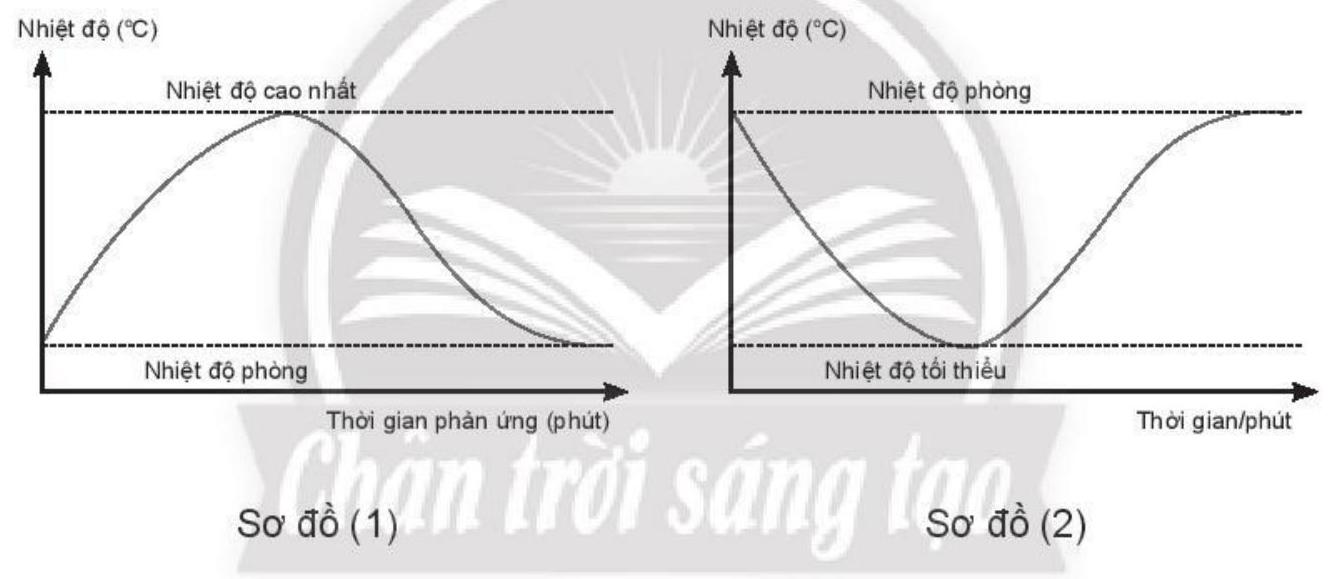
\includegraphics[width=\textwidth]{2025_10_23_883c4b146e2332109fcdg-49}
\captionsetup{labelformat=empty}
\caption{A Sơ đồ biểu diễn sự thay đổi nhiệt độ theo thời gian của phản ứng}
\end{center}
\end{figure}

13.15. Dựa vào Bảng 13.1, SGK trang 84 , viết phương trình nhiệt hoá học của 2 phản ứng sau đây:\\
a) Phản ứng tạo thành $\mathrm{Al}_{2} \mathrm{O}_{3}$.\\
b) Phản ứng tạo thành NO .\\
13.16. Viết phương trình nhiệt hoá học ứng với sơ đồ biểu diễn biến thiên enthalpy của hai phản ứng sau:\\
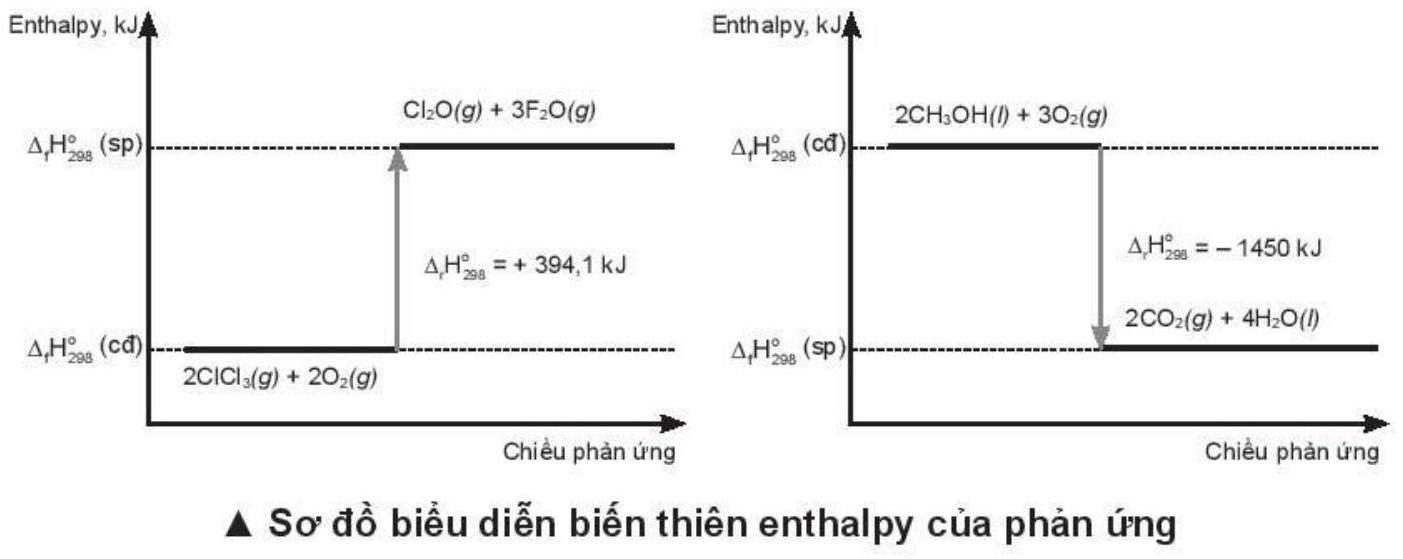
\includegraphics[max width=\textwidth, center]{2025_10_23_883c4b146e2332109fcdg-50}\\
13.17. Cho phản ứng:\\
$2 \mathrm{ZnS}(\mathrm{s})+3 \mathrm{O}_{2}(\mathrm{~g}) \xrightarrow{\mathrm{t}^{\circ}} 2 \mathrm{ZnO}(\mathrm{s})+2 \mathrm{SO}_{2}(\mathrm{~g}) \quad \Delta_{\mathrm{r}} \mathrm{H}_{298}^{\circ}=-285,66 \mathrm{~kJ}$\\
Xác định giá trị của $\Delta_{\mathrm{r}} \mathrm{H}_{298}^{\circ}$ khi:\\
a) Lấy gấp 3 lần khối lượng của các chất phản ứng.\\
b) Lấy một nửa khối lượng của các chất phản ứng.\\
c) Đảo chiều của phản ứng.\\
13.18*. Điều chế $\mathrm{NH}_{3}$ từ $\mathrm{N}_{2}(g)$ và $\mathrm{H}_{2}(g)$ làm nguồn chất tải nhiệt, nguồn để điều chế nitric acid và sản xuất phân urea.

Viết phương trình nhiệt hoá học của phản ứng tạo thành $\mathrm{NH}_{3}$, biết khi sử dụng 7 g khí $\mathrm{N}_{2}$ sinh ra $22,95 \mathrm{~kJ}$ nhiệt.\\
13.19. Viết phương trình nhiệt hoá học của các quá trình tạo thành những chất dưới đây từ đơn chất:\\
a) Nước ở trạng thái khí, biết rằng khi tạo thành 1 mol hơi nước toả ra $214,6 \mathrm{~kJ}$ nhiệt.\\
b) Nước lỏng, biết rằng sự tạo thành 1 mol nước lỏng toả ra $285,49 \mathrm{~kJ}$ nhiệt.\\
c) Ammonia ( $\mathrm{NH}_{3}$ ), biết rằng sự tạo thành $2,5 \mathrm{~g}$ ammonia toả ra $22,99 \mathrm{~kJ}$ nhiệt.\\
d) Phản ứng nhiệt phân đá vôi $\left(\mathrm{CaCO}_{3}\right)$, biết rằng đề thu được $11,2 \mathrm{~g}$ vôi $(\mathrm{CaO})$ phải cung cấp $6,94 \mathrm{kcal}$.\\
13.20. Dựa vào Bảng 13.1, SGK trang 84, sắp xếp các oxide sau đây: $\mathrm{Fe}_{2} \mathrm{O}_{3}(s)$, $\mathrm{Cr}_{2} \mathrm{O}_{3}(s), \mathrm{Al}_{2} \mathrm{O}_{3}(s)$ theo thứ tự giảm dần độ bền nhiệt.

\section*{Bai \\
 14 \\
 \textbackslash section*\{TÍNH BIẾN THIÊN ENTHANPY CỦA PHẢN ỨNG HOÁ HỌC\}}
14.1. Trình bày cách tính enthalpy của phản ứng hoá học dựa vào năng lượng liên kết và dựa vào enthalpy tạo thành của các chất.\\
14.2. Cho phản ứng tổng quát: $\mathrm{aA}+\mathrm{bB} \rightarrow \mathrm{mM}+\mathrm{nN}$. Hãy chọn các phương án tính đúng $\Delta_{\mathrm{r}} \mathrm{H}_{298}^{\circ}$ của phản ứng:\\
(a) $\Delta_{\mathrm{r}} \mathrm{H}^{\circ}{ }_{298 \mathrm{~K}}=\mathrm{m} \times \Delta_{\mathrm{f}} \mathrm{H}_{298}^{\circ}(\mathrm{M})+\mathrm{n} \times \Delta_{\mathrm{f}} \mathrm{H}_{298}^{\circ}(\mathrm{N})-\mathrm{a} \times \Delta_{\mathrm{f}} \mathrm{H}_{298}^{\circ}(\mathrm{A})-\mathrm{b} \times \Delta_{\mathrm{f}} \mathrm{H}_{298}^{\circ}(\mathrm{B})$\\
(b) $\Delta_{\mathrm{r}} \mathrm{H}_{298}^{\circ}=\mathrm{a} \times \Delta_{\mathrm{f}} \mathrm{H}_{298}^{\circ}(\mathrm{A})+\mathrm{b} \times \Delta_{\mathrm{f}} \mathrm{H}_{298}^{\circ}(\mathrm{B})-\mathrm{m} \times \Delta_{\mathrm{f}} \mathrm{H}_{298}^{\circ}(\mathrm{M})-\mathrm{n} \times \Delta_{\mathrm{f}} \mathrm{H}_{298}^{\circ}(\mathrm{N})$\\
(c) $\Delta_{r} H_{298}^{\circ}=a \times E_{b}(A)+b \times E_{b}(B)-m \times E_{b}(M)-n \times E_{b}(N)$\\
(d) $\Delta_{\mathrm{r}} \mathrm{H}_{298}^{\circ}=\mathrm{m} \times \mathrm{E}_{\mathrm{b}}(\mathrm{M})+\mathrm{n} \times \mathrm{E}_{\mathrm{b}}(\mathrm{N})-\mathrm{a} \times \mathrm{E}_{\mathrm{b}}(\mathrm{A})-\mathrm{b} \times \mathrm{E}_{\mathrm{b}}(\mathrm{B})$\\
14.3. Thành phần chính của đa số các loại đá dùng trong xây dựng là $\mathrm{CaCO}_{3}$, chúng vừa có tác dụng chịu nhiệt, vừa chịu được lực. Dựa vào bảng 13.1 SGK trang 84 , tính $\Delta_{\mathrm{r}} \mathrm{H}_{298}^{\circ}$ của phản ứng:

$$
\mathrm{CaCO}_{3}(\mathrm{~s}) \xrightarrow{\mathrm{t}^{\circ}} \mathrm{CaO}(\mathrm{~s})+\mathrm{CO}_{2}(\mathrm{~g})
$$

Phản ứng có xảy ra thuận lợi ở điều kiện thường không?\\
14.4. Propene là nguyên liệu cho sản xuất nhựa polypropylene (PP). PP được sử dụng để sản xuất các sản phẩm ống, màng, dây cách điện, kéo sợi, đồ gia dụng và các sản phẩm tạo hình khác.\\
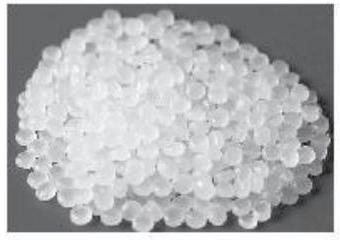
\includegraphics[max width=\textwidth, center]{2025_10_23_883c4b146e2332109fcdg-51(2)}\\
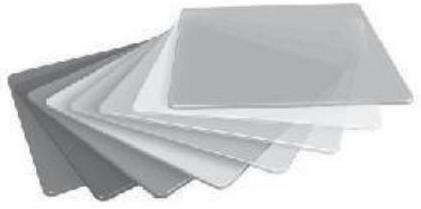
\includegraphics[max width=\textwidth, center]{2025_10_23_883c4b146e2332109fcdg-51(1)}\\
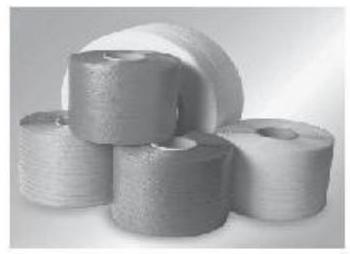
\includegraphics[max width=\textwidth, center]{2025_10_23_883c4b146e2332109fcdg-51}

\begin{itemize}
  \item Các sản phẩm từ nhựa polypropylene (PP)
\end{itemize}

Phản ứng tạo thành propene từ propyne:

$$
\mathrm{CH}_{3}-\mathrm{C} \equiv \mathrm{CH}(\mathrm{~g})+\mathrm{H}_{2}(\mathrm{~g}) \xrightarrow{\mathrm{t}^{\circ}, \mathrm{Pd} / \mathrm{PbCO}_{3}} \mathrm{CH}_{3}-\mathrm{CH}=\mathrm{CH}_{2}(\mathrm{~g})
$$

a) Hãy xác định số liên kết $\mathrm{C}-\mathrm{H} ; \mathrm{C}-\mathrm{C} ; \mathrm{C} \equiv \mathrm{C}$ trong hợp chất $\mathrm{CH}_{3}-\mathrm{C} \equiv \mathrm{CH}$ (propyne).\\
b) Từ năng lượng của các liên kết (Bảng 14.1, SGK trang 89), hãy tính biến thiên enthalpy của phản ứng tạo thành propene trên.\\
14.5. Tính nhiệt tạo thành chuẩn của HF và NO dựa vào năng lượng liên kết (Bảng 14.1 SGK), của $\mathrm{F}_{2}, \mathrm{H}_{2}, \mathrm{HF}, \mathrm{N}_{2}, \mathrm{O}_{2}, \mathrm{NO}$. Giải thích sự khác nhau về nhiệt tạo thành của HF và NO .\\
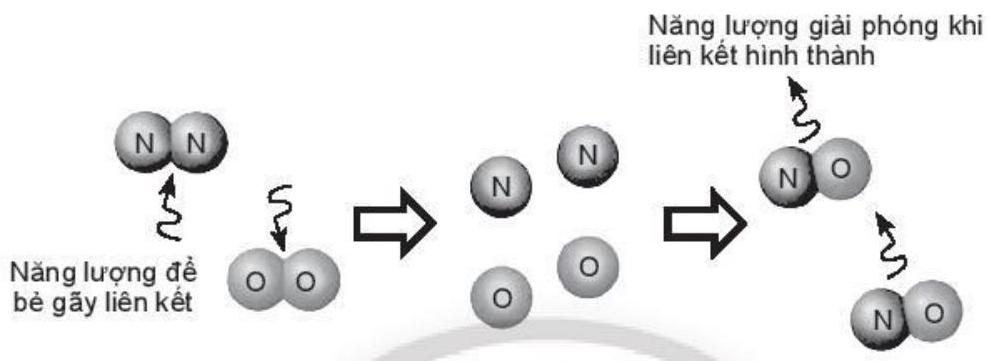
\includegraphics[max width=\textwidth, center]{2025_10_23_883c4b146e2332109fcdg-52(1)}

\section*{- Sự tạo thành NO từ $\mathrm{N}_{2}$ và $\mathrm{O}_{2}$}
14.6. Phosgene là chất khí không màu, mùi cỏ mục, dễ hoá lỏng; khối lượng riêng $1,420 \mathrm{~g} / \mathrm{cm}^{3}$ ( $0^{\circ} 0^{\circ} \mathrm{C}$ ); $\mathrm{t}_{\mathrm{s}}=8,2^{\circ} \mathrm{C}$. Phosgene ít tan trong nướC; dễ tan trong các dung môi hữu cơ, bị thuỷ phân\\
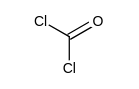
\includegraphics{smile-7112bf2f08ed966b886d2cd5c6982fa95f1d70ba}\\
chậm bằng hơi nước; không cháy; là sản phẩm công nghiệp quan trọng; dùng trong tổng hợp hữu cơ để sản xuất sản phẩm nhuộm, chất diệt cỏ, polyurethane,\\
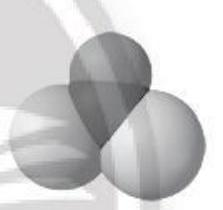
\includegraphics[max width=\textwidth, center]{2025_10_23_883c4b146e2332109fcdg-52}

\begin{itemize}
  \item Hình mô phỏng và công thức phân tử phosgene ( $\mathrm{COCl}_{2}$ )
\end{itemize}

Phosgene là một chất độc. Ở nồng độ $0,005 \mathrm{mg} / \mathrm{L}$ đã nguy hiểm đối với người; trong khoảng $0,1-0,3 \mathrm{mg} / \mathrm{L}$, gây tử vong sau khoảng 15 phút.\\
Phosgene được điều chế bằng cách cho hỗn hợp CO và $\mathrm{Cl}_{2}$ đi qua than hoạt tính. Biết: $\mathrm{E}_{\mathrm{b}}(\mathrm{Cl}-\mathrm{Cl})=243 \mathrm{~kJ} / \mathrm{mol} ; \mathrm{E}_{\mathrm{b}}(\mathrm{C}-\mathrm{Cl})=339 \mathrm{~kJ} / \mathrm{mol} \mathrm{E}_{\mathrm{b}}(\mathrm{C}=\mathrm{O})=745 \mathrm{~kJ} / \mathrm{mol}$; $\mathrm{E}_{\mathrm{b}}(\mathrm{C} \equiv \mathrm{O})=1075 \mathrm{~kJ} / \mathrm{mol}$.

Hãy tính biến thiên enthalpy của phản ứng tạo thành phosgene từ CO và $\mathrm{Cl}_{2}$.\\
14.7. Kim loại nhôm có thể khử được oxide của nhiều nguyên tố. Dựa vào nhiệt tạo thành chuẩn của các chất (Bảng 13.1 SGK), tính biến thiên enthalpy của phản ứng nhôm khử 1 mol mỗi oxide sau:\\
a) $\mathrm{Fe}_{3} \mathrm{O}_{4}(\mathrm{~s})$\\
b) $\mathrm{Cr}_{2} \mathrm{O}_{3}(\mathrm{~s})$.\\
14.8*. Cho 3 hydrocarbon $X, Y, Z$ đều có 2 nguyên tử $C$ trong phân tử. Số nguyên tử H trong các phân tử tăng dần theo thứ tự $\mathrm{X}, \mathrm{Y}, \mathrm{Z}$.\\
a) Viết công thức cấu tạo của $X, Y, Z$.\\
b) Viết phương trình đốt cháy hoàn toàn $X, Y, Z$ với hệ số nguyên tối giản.\\
c) Tính biến thiên enthalpy của mỗi phản ứng dựa vào enthalpy tạo thành tiêu chuẩn trong bảng sau.

\begin{center}
\begin{tabular}{|c|c|c|c|c|c|}
\hline
Chất & $\mathrm{X}(\mathrm{g})$ & $\mathrm{Y}(\mathrm{g})$ & $\mathrm{Z}(\mathrm{g})$ & $\mathrm{CO}_{2}(\mathrm{~g})$ & $\mathrm{H}_{2} \mathrm{O}(\mathrm{g})$ \\
\hline
$\Delta_{\mathrm{f}} \mathrm{H}_{298}^{\circ}(\mathrm{kJ} / \mathrm{mol})$ & $+227,0$ & $+52,47$ & $-84,67$ & $-393,5$ & $-241,82$ \\
\hline
\end{tabular}
\end{center}

d) Từ kết quả tính toán đưa ra kết luận về ứng dụng của phản ứng đốt cháy $X, Y, Z$ trong thực tiễn.\\
14.9. Cho các phản ứng:\\
$\mathrm{CaCO}_{3}(s) \rightarrow \mathrm{CaO}(s)+\mathrm{CO}_{2}(g)$

$$
\Delta_{\mathrm{r}} \mathrm{H}_{298}^{\circ}=+178,49 \mathrm{~kJ}
$$

$\mathrm{C}_{2} \mathrm{H}_{5} \mathrm{OH}(l)+3 \mathrm{O}_{2}(g) \rightarrow 2 \mathrm{CO}_{2}(g)+3 \mathrm{H}_{2} \mathrm{O}(l)$

$$
\Delta_{\mathrm{r}} \mathrm{H}_{298}^{\circ}=-1370,70 \mathrm{~kJ}
$$

C (graphite, $s$ ) $+\mathrm{O}_{2}(g) \rightarrow \mathrm{CO}_{2}(g)$

$$
\Delta_{\mathrm{r}} \mathrm{H}_{298}^{\circ}=-393,51 \mathrm{~kJ}
$$

a) Phản ứng nào có thể tự xảy ra (sau giai đoạn khơi mào ban đầu), phản ứng nào không thể tự xảy ra?\\
b) Khối lượng ethanol hay graphite cần dùng khi đốt cháy hoàn toàn đủ tạo lượng nhiệt cho quá trình nhiệt phân hoàn toàn $0,1 \mathrm{~mol} \mathrm{CaCO}_{3}$. Giả thiết hiệu suất các quá trình đều là $100 \%$.\\
14.10. Lactic acid hay acid sữa là hợp chất hoá học đóng vai trò quan trọng trong nhiều quá trình sinh hoá, lần đầu tiên được phân tách vào năm 1780 bởi nhà hoá học Thuy. Điển Carl Wilhelm Scheele. Lactic acid

\begin{figure}[h]
\begin{center}
  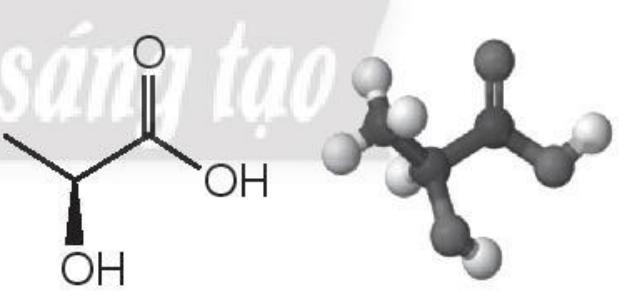
\includegraphics[width=\textwidth]{2025_10_23_883c4b146e2332109fcdg-53}
\captionsetup{labelformat=empty}
\caption{- Công thức phân tử và mô hình phân tử lactic acid}
\end{center}
\end{figure}

có công thức phân tử $\mathrm{C}_{3} \mathrm{H}_{6} \mathrm{O}_{3}$, công thức cấu tạo $\mathrm{CH}_{3}-\mathrm{CH}(\mathrm{OH})-\mathrm{COOH}$ Khi vận động mạnh cơ thể không đủ cung cấp oxygen, thì cơ thể sẽ chuyển hoá glucose thành lactic acid từ các tế bào để cung cấp năng lượng cho cơ thể (lactic acid tạo thành từ quá trình này sẽ gây mỏi cơ) theo phương trình sau:

$$
\mathrm{C}_{6} \mathrm{H}_{12} \mathrm{O}_{6}(a q) \rightarrow 2 \mathrm{C}_{3} \mathrm{H}_{6} \mathrm{O}_{3}(a q) \quad \Delta_{\mathrm{r}} \mathrm{H}_{298}^{\circ}=-150 \mathrm{~kJ}
$$

Biết rằng cơ thể chỉ cung cấp $98 \%$ năng lượng nhờ oxygen, năng lượng còn lại nhờ vào sự chuyển hoá glucose thành lactic acid.

Giả sử một người chạy bộ trong một thời gian tiêu tốn 300 kcal. Tính khối lượng lactic acid tạo ra từ quá trình chuyển hoá đó (biết $1 \mathrm{cal}=4,184 \mathrm{~J}$ ).\\
14.11. Chloromethane $\left(\mathrm{CH}_{3} \mathrm{Cl}\right)$, còn được gọi là methyl chloride, Refrigerant- 40 hoặc $\mathrm{HCC} 40 . \mathrm{CH}_{3} \mathrm{Cl}$ từng được sử dụng rộng rãi như một chất làm lạnh. Hợp chất khí này rất dễ cháy, có thể không mùi hoặc có mùi thơm nhẹ.\\
Từ năng lượng của các liên kết (Bảng 14.1 SGK), hãy tính biến thiên enthalpy của phản ứng tạo thành chloromethane:

$$
\mathrm{CH}_{4}(g)+\mathrm{Cl}_{2}(g) \rightarrow \mathrm{CH}_{3} \mathrm{Cl}(g)+\mathrm{HCl}(g)
$$

Cho biết phản ứng dễ dàng xảy ra dưới ánh sáng mặt trời. Kết quả tính có mâu thuẫn với khả năng dễ xảy ra của phản ứng không.\\
14.12*. Một xe tải đang vận chuyển đất đèn (thành phần chính là $\mathrm{CaC}_{2}$ và CaO ) gặp mưa xảy ra sự cố, xe tải đã bốc cháy.\\
a) Viết phản ứng của $\mathrm{CaC}_{2}$ và CaO với nước.\\
b) Xe tải bốc cháy do các phản ứng trên toả nhiệt kích thích phản ứng cháy của acetylene:

$$
\mathrm{C}_{2} \mathrm{H}_{2}(g)+2,5 \mathrm{O}_{2}(g) \xrightarrow{\mathrm{t}^{\circ}} 2 \mathrm{CO}_{2}(g)+\mathrm{H}_{2} \mathrm{O}(g)
$$

Dựa vào Bảng 13.1 SGK, tính biến thiên enthalpy của các phản ứng trên. Cho biết phản ứng toả nhiệt hay thu nhiệt.\\
14.13. Cho phương trình hoá học của phản ứng:

$$
\mathrm{C}_{2} \mathrm{H}_{4}(g)+\mathrm{H}_{2} \mathrm{O}(l) \rightarrow \mathrm{C}_{2} \mathrm{H}_{5} \mathrm{OH}(l)
$$

Tính biến thiên enthalpy của phản ứng theo nhiệt tạo thành chuẩn của các chất (Bảng 13.1 SGK).\\
14.14*. Cho phản ứng phân huỷ hydrazine: $\mathrm{N}_{2} \mathrm{H}_{4}(g) \rightarrow \mathrm{N}_{2}(g)+2 \mathrm{H}_{2}(g)$\\
a) Tính $\Delta_{\mathrm{r}} \mathrm{H}_{298}^{\circ}$ theo năng lượng liên kết của phản ứng trên.\\
b) Hydrazine $\left(\mathrm{N}_{2} \mathrm{H}_{4}\right)$ là chất lỏng ở điều kiện thường (sôi ở $114^{\circ} \mathrm{C}$, khối lượng riêng $1,021 \mathrm{~g} / \mathrm{cm}^{3}$ ). Hãy đề xuất lí do $\mathrm{N}_{2} \mathrm{H}_{4}$ được sử dụng làm nhiên liệu trong động cơ tên lửa. Biết: $\mathrm{E}_{\mathrm{b}}(\mathrm{N}-\mathrm{N})=160 \mathrm{~kJ} / \mathrm{mol} ; \mathrm{E}_{\mathrm{b}}(\mathrm{N}-\mathrm{H})=391 \mathrm{~kJ} / \mathrm{mol}$; $\mathrm{E}_{\mathrm{b}}(\mathrm{N} \equiv \mathrm{N})=945 \mathrm{~kJ} / \mathrm{mol}, \mathrm{E}_{\mathrm{b}}(\mathrm{H}-\mathrm{H})=432 \mathrm{~kJ} / \mathrm{mol}$.\\
14.15. Quá trình hoà tan calcium chloride trong nước:

$$
\mathrm{CaCl}_{2}(s) \rightarrow \mathrm{Ca}^{2+}(a q)+2 \mathrm{Cl}^{-}(a q) \quad \Delta_{\mathrm{r}} \mathrm{H}_{298}^{\circ}=?
$$

\begin{center}
\begin{tabular}{|c|c|c|c|}
\hline
Chất & $\mathrm{CaCl}_{2}$ & $\mathrm{Ca}^{2+}$ & $\mathrm{Cl}^{-}$ \\
\hline
$\Delta_{\mathrm{f}} \mathrm{H}^{\circ}{ }_{298}(\mathrm{~kJ} / \mathrm{mol})$ & $-795,0$ & $-542,83$ & $-167,16$ \\
\hline
\end{tabular}
\end{center}

Tính biến thiên enthalpy của quá trình.

\section*{ÔN TẬP CHƯONG 5}
OT5.1. Tìm hiểu và giải thích 2 quá trình sau:\\
a) Tại sao khi xoa cồn vào da, ta cảm thấy lạnh?\\
b) Phản ứng phân huỷ $\mathrm{Fe}(\mathrm{OH})_{3}(s)$ phải cung cấp nhiệt độ liên tục.

OT5.2. Cho phương trình nhiệt hoá học của phản ứng sau:\\
C(kim cương) $\longrightarrow$ C(graphite)

$$
\Delta_{\mathrm{r}} \mathrm{H}_{298}^{\circ}=-1,9 \mathrm{~kJ}
$$

Kim cương hay graphite là dạng bền hơn của carbon?\\
OT5.3. Cho hai phương trình nhiệt hoá học sau:


\begin{equation*}
\mathrm{CO}(g)+\frac{1}{2} \mathrm{O}_{2}(g) \rightarrow \mathrm{CO}_{2}(g) \tag{1}
\end{equation*}


$$
\Delta_{\mathrm{r}} \mathrm{H}_{298}^{\circ}=-283,00 \mathrm{~kJ}
$$


\begin{equation*}
\mathrm{H}_{2}(g)+\mathrm{F}_{2}(g) \rightarrow 2 \mathrm{HF}(g) \tag{2}
\end{equation*}


$$
\Delta_{\mathrm{r}} \mathrm{H}_{298}^{\circ}=-546,00 \mathrm{~kJ}
$$

So sánh nhiệt giữa hai phản ứng (1) và (2). Phản ứng nào xảy ra thuận lợi hơn?\\
OT5.4. Cho hai phương trình nhiệt hoá học sau:\\
$\mathrm{CO}(g)+\frac{1}{2} \mathrm{O}_{2}(g) \rightarrow \mathrm{CO}_{2}(g)$

$$
\Delta_{\mathrm{r}} \mathrm{H}_{298}^{\circ}=-283,00 \mathrm{~kJ}
$$

$\mathrm{C}_{2} \mathrm{H}_{5} \mathrm{OH}(l)+\frac{7}{2} \mathrm{O}_{2}(g) \rightarrow 2 \mathrm{CO}_{2}(g)+3 \mathrm{H}_{2} \mathrm{O}(l)$

$$
\Delta_{\mathrm{r}} \mathrm{H}_{298}^{\circ}=-1366,89 \mathrm{~kJ}
$$

Khi đốt cháy cùng 1 mol CO và $\mathrm{C}_{2} \mathrm{H}_{5} \mathrm{OH}$ thì phản ứng nào toả ra lượng nhiệt lớn hơn?

OT5.5. Cho phương trình nhiệt hoá học sau:

$$
\mathrm{H}_{2}(g)+\mathrm{F}_{2}(g) \rightarrow 2 \mathrm{HF}(g)
$$

$$
\Delta_{\mathrm{r}} \mathrm{H}_{298}^{\circ}=-546,00 \mathrm{~kJ}
$$

Vẽ sơ đồ biểu diễn biến thiên enthalpy của phản ứng.\\
OT5.6. Cho các phương trình nhiệt hoá học sau:

$$
\begin{array}{ll}
2 \mathrm{H}_{2}(g)+\mathrm{O}_{2}(g) \rightarrow 2 \mathrm{H}_{2} \mathrm{O}(l) & \Delta_{\mathrm{r}} \mathrm{H}_{298}^{\circ}=-571,68 \mathrm{~kJ} \\
\frac{1}{2} \mathrm{H}_{2}(g)+\frac{1}{2} \mathrm{I}_{2}(g) \rightarrow \mathrm{HI}(g) & \Delta_{\mathrm{r}} \mathrm{H}_{298}^{\circ}=+25,9 \mathrm{~kJ}
\end{array}
$$

Xác định biến thiên enthalpy của 2 phản ứng sau:

$$
\begin{array}{ll}
\mathrm{H}_{2}(g)+\frac{1}{2} \mathrm{O}_{2}(g) \rightarrow \mathrm{H}_{2} \mathrm{O}(l) & \Delta_{\mathrm{r}} \mathrm{H}_{298}^{\circ}=? \\
\mathrm{HI}(g) \rightarrow \frac{1}{2} \mathrm{H}_{2}(g)+\frac{1}{2} \mathrm{I}_{2}(g) & \Delta_{\mathrm{r}} \mathrm{H}_{298}^{\circ}=?
\end{array}
$$

OT5.7. Mỗi quá trình dưới đây là tự diễn ra hay không?\\
a) Cho $\mathrm{CaC}_{2}$ vào nước, khí $\mathrm{C}_{2} \mathrm{H}_{2}$ thoát ra.\\
b) Khí CO khử FeO ở nhiệt độ phòng.\\
c) Các phân tử nước được chuyển thành khí hydrogen và oxygen.

Với quá trình không tự diễn ra, dự đoán giá trị của nhiệt phản ứng.\\
OT5.8. Thí nghiệm phân huỷ hydrogen peroxide $\left(\mathrm{H}_{2} \mathrm{O}_{2}\right)$ thành nước và khí oxygen có xúc tác KI theo phương trình nhiệt hoá học sau:

$$
2 \mathrm{H}_{2} \mathrm{O}_{2}(\mathrm{aq}) \xrightarrow{\mathrm{KI}} \mathrm{O}_{2}(\mathrm{~g})+2 \mathrm{H}_{2} \mathrm{O}(\mathrm{l}) \quad \Delta_{\mathrm{r}} \mathrm{H}_{298}^{\circ}=-196 \mathrm{~kJ}
$$

Phản ứng trên là phản ứng thu nhiệt hay toả nhiệt? Hãy đề xuất cách chứng $\operatorname{minh}$ khí sinh ra là oxygen. Nêu ứng dụng của thí nghiệm trên trong thực tiễn.

OT5.9. Cho phương trình nhiệt hoá học sau:

$$
\mathrm{NaOH}(a q)+\mathrm{HCl}(a q) \rightarrow \mathrm{NaCl}(a q)+\mathrm{H}_{2} \mathrm{O}(l) \quad \Delta_{\mathrm{r}} \mathrm{H}_{298}^{\circ}=-57,3 \mathrm{~kJ}
$$

a) Vẽ sơ đồ biểu diễn biến thiên enthalpy của phản ứng.\\
b) Tính lượng nhiệt toả ra khi dùng dung dịch có chứa 8 g NaOH trung hoà với lượng vừa đủ dung dịch HCl .

OT5.10*. Phản ứng của glycerol với nitric acid (khử nước) tạo thành trinitroglycerin $\left(\mathrm{C}_{3} \mathrm{H}_{5} \mathrm{O}_{3}\left(\mathrm{NO}_{2}\right)_{3}\right)$. Trinitroglycerin là một loại thuốc nổ, khi phân huỷ tạo thành sản phẩm gồm có nitrogen, oxygen, carbon dioxide và hơi nước.\\
a) Viết phương trình phản ứng hoá học của phản ứng điều chế trinitroglycerin từ glycerol với nitric acid và phản ứng phân huỷ của trinitroglycerin\\
b) Nếu phân huỷ $45,4 \mathrm{~g}$ trinitroglycerin, tính số mol khí và hơi tạo thành.\\
c) Khi phân huỷ 1 mol trinitroglycerin tạo thành 1448 kJ nhiệt lượng. Tính Iượng nhiệt tạo thành khi phân huỷ 1 kg trinitroglycerin.

OT5.11. Cho các phương trình nhiệt hoá học của phản ứng:\\
a) $3 \mathrm{H}_{2}(g)+\frac{3}{2} \mathrm{O}_{2}(g) \rightarrow 3 \mathrm{H}_{2} \mathrm{O}(l) \Delta_{\mathrm{r}} \mathrm{H}_{298}^{\circ}=-857,52 \mathrm{~kJ}$\\
b) $2 \mathrm{~S}(s)+3 \mathrm{O}_{2}(g) \rightarrow 2 \mathrm{SO}_{3}(g) \Delta_{\mathrm{r}} \mathrm{H}_{298}^{\circ}=+792,2 \mathrm{~kJ}$

Ở điều kiện chuẩn nếu đốt cháy hoàn toàn $1,2 \mathrm{~g} \mathrm{H}_{2}(\mathrm{a})$ và $3,2 \mathrm{~g} \mathrm{~S}(\mathrm{~b})$ thì lượng nhiệt toả ra hay cần cung cấp là bao nhiêu?

OT5.12. Tìm hiểu ứng dụng của silver bromide $(\mathrm{AgBr})$ trên phim ảnh. Phản ứng xảy ra là toả nhiệt hay thu nhiệt? Giải thích.

OT5.13. Glucose là một loại monosaccarit với công thức phân tử $\mathrm{C}_{6} \mathrm{H}_{12} \mathrm{O}_{6}$ được tạo ra bởi thực vật và hầu hết các loại tảo trong quá trình quang hợp từ nước và $\mathrm{CO}_{2}$, sử dụng năng lượng từ ánh sáng mặt trời. Dung dịch glucose $5 \% (\mathrm{D}=1,1 \mathrm{~g} / \mathrm{mL})$ là dung dịch đường tiêm tĩnh mạch, là loại thuốc thiết yếu, quan trọng của Tổ chức Y tế Thế giới (WHO) và hệ thống y tế cơ bản. Phương trình nhiệt hoá học của phản ứng oxi hoá glucose:

$$
\mathrm{C}_{6} \mathrm{H}_{12} \mathrm{O}_{6}(\mathrm{~s})+6 \mathrm{O}_{2}(\mathrm{~g}) \rightarrow 6 \mathrm{CO}_{2}(\mathrm{~g})+6 \mathrm{H}_{2} \mathrm{O}(\mathrm{l}) \quad \Delta_{\mathrm{r}} \mathrm{H}_{298}^{\circ}=-2803,0 \mathrm{~kJ}
$$

Tính năng lượng tối đa khi một người bệnh được truyền 1 chai 500 mL dung dịch glucose $5 \%$.

OT5.14. Khí gas chứa chủ yếu các thành phần chính: Propane $\left(\mathrm{C}_{3} \mathrm{H}_{8}\right)$, butane $\left(\mathrm{C}_{4} \mathrm{H}_{10}\right)$ và một số thành phần khác. Để tạo mùi cho gas nhà sản xuất đã pha trộn thêm chất tạo mùi đặc trưng như methanethiol $\left(\mathrm{CH}_{3} \mathrm{SH}\right)$, có mùi giống tỏi, hành tây. Trong thành phần khí gas, tỉ lệ hoà trộn phổ biến của propane: butane theo thsứ tự là $30: 70$ đến $50: 50$.\\
a) Mục đích việc pha trộn thêm chất tạo mùi đặc trưng vào khí gas là gì?\\
b) Cho các phương trình nhiệt hoá học sau:

$$
\begin{array}{ll}
\mathrm{C}_{3} \mathrm{H}_{8}(s)+5 \mathrm{O}_{2}(g) \rightarrow 3 \mathrm{CO}_{2}(g)+4 \mathrm{H}_{2} \mathrm{O}(l) & \Delta_{\mathrm{r}} \mathrm{H}_{298}^{\circ}=-2220 \mathrm{~kJ} \\
\mathrm{C}_{4} \mathrm{H}_{10}(s)+\frac{13}{2} \mathrm{O}_{2}(g) \rightarrow 4 \mathrm{CO}_{2}(g)+5 \mathrm{H}_{2} \mathrm{O}(l) & \Delta_{\mathrm{r}} \mathrm{H}_{298}^{\circ}=-2874 \mathrm{~kJ}
\end{array}
$$

Tính nhiệt lượng toả ra khi đốt cháy hoàn toàn 1 bình gas 12 kg với tỉ lệ thể tích của propane : butane là $30: 70$ (thành phần khác không đáng kể) ở điều kiện chuẩn.\\
c) Giả sử một hộ gia đình cần 6000 kJ nhiệt mỗi ngày, sau bao nhiêu ngày sẽ sử dụng hết 1 bình gas (với hiệu suất hấp thụ nhiệt khoảng $60 \%$ )?

\section*{Chương 6. TỐC ĐỘ PHẢN ÚNG HOÁ HỌC}
\section*{15}
\section*{PHƯƠNG TRİNH TỐC ĐỘ PHẢN ÚNG VÀ HẰNG SỐ TỐC ĐỘ PHẢN ỨNG}
15.1. Cho phương trình hoá học:\\
$2 \mathrm{KMnO}_{4}(a q)+10 \mathrm{FeSO}_{4}(a q)+8 \mathrm{H}_{2} \mathrm{SO}_{4}(a q) \rightarrow 5 \mathrm{Fe}_{2}\left(\mathrm{SO}_{4}\right)_{3}(a q)+\mathrm{K}_{2} \mathrm{SO}_{4}(a q)+2 \mathrm{MnSO}_{4}(a q)+8 \mathrm{H}_{2} \mathrm{O}(l)$\\
Với cùng một lượng các chất tham gia phản ứng, chất phản ứng hết nhanh nhất là:\\
A. $\mathrm{KMnO}_{4}$.\\
B. $\mathrm{FeSO}_{4}$.\\
C. $\mathrm{H}_{2} \mathrm{SO}_{4}$.\\
D. Cả 3 chất hết cùng lúc.\\
15.2. Đối với phản ứng: $A+3 B \rightarrow 2 C$, phát biểu nào sau đây đúng?\\
A. Tốc độ tiêu hao chất $B$ bằng $3 / 2$ tốc độ tạo thành chất $C$.\\
B. Tốc độ tiêu hao chất $B$ bằng $2 / 3$ tốc độ tạo thành chất $C$.\\
C. Tốc độ tiêu hao chất B bằng 3 tốc độ tạo thành chất C .\\
D. Tốc độ tiêu hao chất $B$ bằng $1 / 3$ tốc độ tạo thành chất $C$.\\
15.3. Biểu đồ nào sau đây không biểu diễn sự phụ thuộc nồng độ chất tham gia với thời gian

\begin{figure}[h]
\begin{center}
\captionsetup{labelformat=empty}
\caption{A.}
  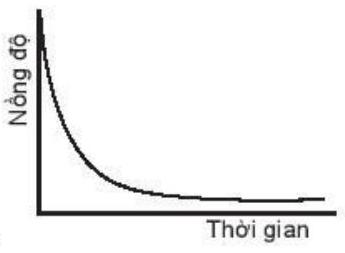
\includegraphics[width=\textwidth]{2025_10_23_883c4b146e2332109fcdg-58(3)}
\end{center}
\end{figure}

\begin{figure}[h]
\begin{center}
\captionsetup{labelformat=empty}
\caption{B.}
  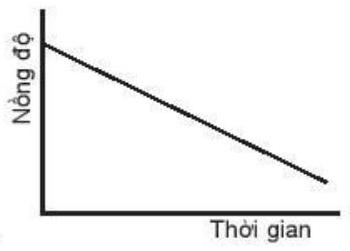
\includegraphics[width=\textwidth]{2025_10_23_883c4b146e2332109fcdg-58}
\end{center}
\end{figure}

\begin{figure}[h]
\begin{center}
\captionsetup{labelformat=empty}
\caption{C.}
  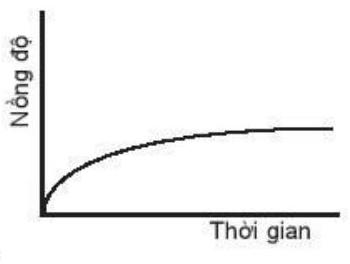
\includegraphics[width=\textwidth]{2025_10_23_883c4b146e2332109fcdg-58(2)}
\end{center}
\end{figure}

\begin{figure}[h]
\begin{center}
\captionsetup{labelformat=empty}
\caption{D.}
  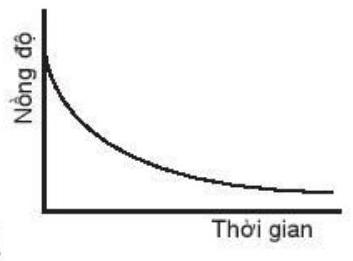
\includegraphics[width=\textwidth]{2025_10_23_883c4b146e2332109fcdg-58(1)}
\end{center}
\end{figure}

15.4. Đồ thị biểu diễn đường cong động học của phản ứng giữa oxygen và hydrogen tạo thành nước, $\mathrm{O}_{2}(g)+2 \mathrm{H}_{2}(g) \rightarrow 2 \mathrm{H}_{2} \mathrm{O}(g)$. Đường cong nào của hydrogen?\\
A. Đường cong số (1).\\
B. Đường cong số (2).\\
C. Đường cong số (3).\\
D. Đường cong số (2) hoặc (3) đều đúng.\\
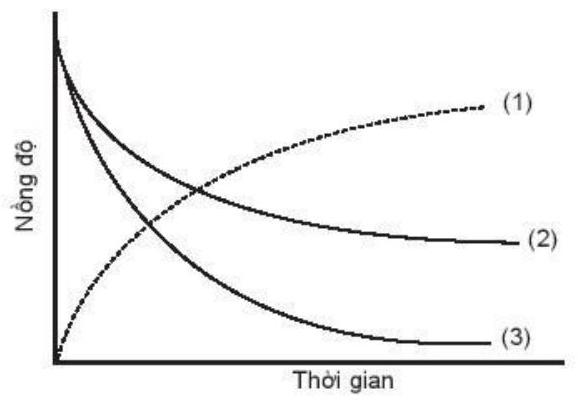
\includegraphics[max width=\textwidth, center]{2025_10_23_883c4b146e2332109fcdg-59}\\
15.5. Phương trình tổng hợp ammonia $\left(\mathrm{NH}_{3}\right), \mathrm{N}_{2}(g)+3 \mathrm{H}_{2}(g) \rightarrow 2 \mathrm{NH}_{3}(g)$. Nếu tốc độ tạo thành $\mathrm{NH}_{3}$ là $0,345 \mathrm{M} / \mathrm{s}$ thì tốc độ của chất phản ứng $\mathrm{H}_{2}$ là\\
A. $0,345 \mathrm{M} / \mathrm{s}$.\\
B. $0,690 \mathrm{M} / \mathrm{s}$.\\
C. $0,173 \mathrm{M} / \mathrm{s}$.\\
D. $0,518 \mathrm{M} / \mathrm{s}$.\\
15.6. Phương trình hoá học của phản ứng: $\mathrm{CHCl}_{3}(g)+\mathrm{Cl}_{2}(g) \rightarrow \mathrm{CCl}_{4}(g)+\mathrm{HCl}(g)$. Khi nồng độ của $\mathrm{CHCl}_{3}$ giảm 4 lần, nồng độ $\mathrm{Cl}_{2}$ giữ nguyên thì tốc độ phản ứng sẽ\\
A. tăng gấp đôi.\\
B. giảm một nửa.\\
C. tăng 4 lần.\\
D. giảm 4 lần.\\
15.7. Cho phương trình hoá học của phản ứng:

$$
\mathrm{CO}(g)+\mathrm{H}_{2} \mathrm{O}(g) \rightarrow \mathrm{CO}_{2}(g)+\mathrm{H}_{2}(g)
$$

Viết biểu thức tốc độ của phản ứng trên. Khi nồng độ CO tăng 2 lần, lượng hơi nước không thay đổi, tốc độ phản ứng thay đổi như thế nào?\\
15.8. Từ dữ kiện trong Ví dụ 1 (SGK trang 95 ), tính tốc độ trung bình của phản ứng theo giá trị nồng độ của $\mathrm{MgCl}_{2}$ trong 40 giây (bỏ qua sự thay đổi không đáng\\
kể về thể tích dung dịch sau phản ứng). So sánh giá trị tốc độ phản ứng tính theo HCl với tính theo $\mathrm{MgCl}_{2}$.\\
15.9. Một số phản ứng diễn ra với số mol chất phản ứng cụ thể theo thời gian được thể hiện trong bảng dưới đây:

\begin{center}
\begin{tabular}{|l|l|l|l|}
\hline
Phản ứng & Lượng chất phản ứng (mol) & Thời gian (s) & Tốc độ phản ứng (mol/s) \\
\hline
1 & 2 & 30 & ? \\
\hline
2 & 5 & 120 & ? \\
\hline
3 & 1 & 90 & ? \\
\hline
4 & 3,2 & 90 & ? \\
\hline
5 & 5,9 & 30 & ? \\
\hline
\end{tabular}
\end{center}

a) Tính tốc độ trung bình của mỗi phản ứng\\
b) Phản ứng nào diến ra với tốc độ nhanh nhất? Phản ứng nào diễn ra với tốc độ chậm nhất?\\
15.10. Hai phương trình hoá học của phản ứng xảy ra với cùng một lượng $\mathrm{Cl}_{2}$ như sau:


\begin{align*}
& \mathrm{Mg}(s)+\mathrm{Cl}_{2}(g) \rightarrow \mathrm{MgCl}_{2}(s)  \tag{1}\\
& 2 \mathrm{Na}(s)+\mathrm{Cl}_{2}(g) \rightarrow 2 \mathrm{NaCl}(s) \tag{2}
\end{align*}


Sau 1 phút, khối lượng $\mathrm{MgCl}_{2}$ được tạo ra 2 gam.\\
a) Tính tốc độ trung bình ( $\mathrm{mol} / \mathrm{s}$ ) của phản ứng (1).\\
b) Nếu tốc độ trung bình xảy ra trong phản ứng (2) tương đương (1), thì khối lượng sản phẩm NaCl thu được là bao nhiêu?\\
15.11. Cho phản ứng tert-butyl chloride (tert- $\mathrm{C}_{4} \mathrm{H}_{9} \mathrm{Cl}$ ) với nước:

$$
\mathrm{C}_{4} \mathrm{H}_{9} \mathrm{Cl}(l)+\mathrm{H}_{2} \mathrm{O}(l) \rightarrow \mathrm{C}_{4} \mathrm{H}_{9} \mathrm{OH}(a q)+\mathrm{HCl}(a q)
$$

Tính tốc độ trung bình của phản ứng theo tert-butyl chloride, với nồng độ ban đầu là $0,22 \mathrm{M}$, sau 4 s , nồng độ còn lại $0,10 \mathrm{M}$.\\
15.12. Xét phản ứng hoá học đơn giản giữa hai chất $A$ và $B$ theo phương trình: $A+B \rightarrow C$. Từ thông tin đã cho, hoàn thành bảng dưới đây:

\begin{center}
\begin{tabular}{|l|l|l|l|}
\hline
Thực nghiệm & Nồng độ chất $A$ (M) & Nồng độ chất B (M) & Tốc độ phản ứng (M/s) \\
\hline
1 & 0,20 & 0,050 & 0,24 \\
\hline
2 & ? & 0,030 & 0,20 \\
\hline
3 & 0,40 & ? & 0,80 \\
\hline
\end{tabular}
\end{center}

15.13. Xét phản ứng phân huỷ khí $\mathrm{N}_{2} \mathrm{O}_{5}$ xảy ra như sau:

$$
2 \mathrm{~N}_{2} \mathrm{O}_{5}(g) \rightarrow 4 \mathrm{NO}_{2}(g)+\mathrm{O}_{2}(g)
$$

a) Viết biểu thức tính tốc độ phản ứng theo sự biến thiên nồng độ của chất tham gia và sản phẩm theo thời gian.\\
b) Sau khoảng thời gian $\mathrm{t}(\mathrm{s})$, tốc độ tạo thành $\mathrm{O}_{2}$ là $9,0 \times 10^{-6}(\mathrm{M} / \mathrm{s})$, tính tốc độ của các chất còn lại trong phản ứng.\\
15.14. Sulfuric acid $\left(\mathrm{H}_{2} \mathrm{SO}_{4}\right)$ là hoá chất quan trọng trong công nghiệp, ứng dụng trong sản xuất phân bón, lọc dầu, xử lí nước thải, ... Một giai đoạn để sản xuất $\mathrm{H}_{2} \mathrm{SO}_{4}$ là phản ứng $2 \mathrm{SO}_{2}(\mathrm{~g})+\mathrm{O}_{2}(\mathrm{~g}) \rightarrow 2 \mathrm{SO}_{3}(\mathrm{~g})$, kết quả thực nghiệm của phản ứng cho giá trị theo bảng:

\begin{center}
\begin{tabular}{|l|l|l|l|}
\hline
Thời gian (s) & $\mathbf{S O}_{\mathbf{2}} \boldsymbol{(} \mathbf{M} \boldsymbol{)}$ & $\mathbf{O}_{\mathbf{2}} \boldsymbol{(} \mathbf{M} \boldsymbol{)}$ & $\mathrm{SO}_{3}$ (M) \\
\hline
300 & 0,0270 & 0,0500 & 0,0072 \\
\hline
720 & 0,0194 & 0,0462 & 0,0148 \\
\hline
\end{tabular}
\end{center}

Tính tốc độ trung bình của phản ứng trong khoảng thời gian trên.

\section*{16}
\section*{CÁC YẾU TỐ ẢNH HUỞNG ĐẾN TỐC ĐỘ PHẢN ÚNG HOÁ HỌC}
16.1. Khi tăng nồng độ chất tham gia, thì\\
A. tốc độ phản ứng tăng.\\
B. tốc độ phản ứng giảm.\\
C. không ảnh hưởng đến tốc độ phản ứng.\\
D. có thể tăng hoặc giảm tốc độ phản ứng.\\
16.2. Yếu tố nào sau đây làm giảm tốc độ phản ứng:\\
A. Sử dụng enzyme cho phản ứng.\\
B. Thêm chất ức chế vào hỗn hợp chất tham gia.\\
C. Tăng nồng độ chất tham gia.\\
D. Nghiền chất tham gia dạng khối thành bột.\\
16.3. Các enzyme là chất xúc tác, có chức năng:\\
A. Giảm năng lượng hoạt hoá của phản ứng.\\
B. Tăng năng lượng hoạt hoá của phản ứng.\\
C. Tăng nhiệt độ của phản ứng.\\
D. Giảm nhiệt độ của phản ứng.\\
16.4. Yếu tố nào dưới đây không ảnh hưởng đến tốc độ phản ứng:\\
A. Nhiệt độ chất phản ứng.\\
B. Thể vật lí của chất phản ứng (rắn, lỏng, kích thước lớn, nhỏ, ...).\\
C. Nồng độ chất phản ứng.\\
D. Tỉ trọng của chất phản ứng.\\
16.5. Sản phẩm của phản ứng được tạo ra qua các bước theo hình bên dưới:\\
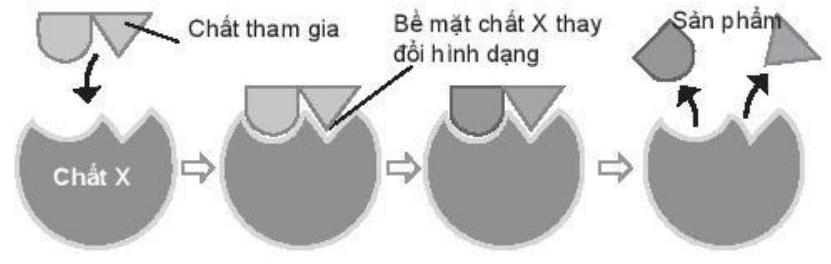
\includegraphics[max width=\textwidth, center]{2025_10_23_883c4b146e2332109fcdg-62}

Vai trò của chất X là\\
A. chất xúc tác.\\
B. làm tăng năng lượng hoạt hoá của chất tham gia phản ứng.\\
C. Iàm giảm năng lượng hoạt hoá của chất tham gia phản ứng.\\
D. làm tăng nồng độ chất tham gia phản ứng.\\
16.6. Tốc độ của một phản ứng hoá học\\
A. chỉ phụ thuộc vào nồng độ các chất tham gia phản ứng.\\
B. tăng khi nhiệt độ của phản ứng tăng.\\
C. càng nhanh khi giá trị năng lượng hoạt hoá càng lớn.\\
D. không phụ thuộc vào diện tích bề mặt.\\
16.7. Hoàn thành bảng sau, cho biết mỗi thay đổi sẽ làm tăng hay giảm tốc độ của phản ứng

\begin{center}
\begin{tabular}{|l|l|}
\hline
Yếu tố ảnh hưởng & Tốc độ phản ứng \\
\hline
Đun nóng chất tham gia & Tăng \\
\hline
Thêm xúc tác phù hợp &  \\
\hline
Pha loãng dung dịch &  \\
\hline
Ngưng dùng enzyme (chất xúc tác) &  \\
\hline
Giảm nhiệt độ &  \\
\hline
Tăng nhiệt độ &  \\
\hline
Giảm diện tích bề mặt &  \\
\hline
Tăng nồng độ chất phản ứng &  \\
\hline
Chia nhỏ chất phản ứng thành mảnh nhỏ &  \\
\hline
\end{tabular}
\end{center}

16.8. Có 3 phương pháp chính được sử dụng để tăng tốc độ của phản ứng hoá học: tăng nồng độ, tăng nhiệt độ và thêm chất xúc tác. Theo lí thuyết va chạm, hãy giải thích 3 phương pháp đó.\\
16.9. Hoàn thành bảng sau, cho biết yếu tố chính ảnh hưởng đến tốc độ phản ứng trong từng trường hợp

\begin{center}
\begin{tabular}{|l|l|}
\hline
Tình huống & Yếu tố ảnh hưởng \\
\hline
Duy trì thổi không khí vào bếp để than cháy đều &  \\
\hline
Than đá được nghiền nhỏ dùng trong quá trình luyện kim loại &  \\
\hline
Thức ăn được tiêu hoá trong dạ dày nhờ acid và enzyme &  \\
\hline
Xác của một số loài động vật được bảo quản nguyên vẹn ở Bắc cực và Nam cực hàng ngàn năm &  \\
\hline
Vụ nổ bụi xảy ra tại một xưởng cưa &  \\
\hline
\end{tabular}
\end{center}

16.10. Trong thí nghiệm 3 (SGK trang 102), người ta cân khối lượng chất rắn trước và sau phản ứng thấy không đổi, chứng tỏ chất xúc tác có tham gia như là một chất phản ứng không? Giải thích.\\
16.11. Tốc độ các phản ứng sau chịu ảnh hưởng của yếu tố nào?\\
a) Than củi đang cháy, dùng quạt thổi thêm không khí vào, sự cháy diễn ra mạnh hơn.\\
b) Phản ứng oxi hoá $\mathrm{SO}_{2}$ thành $\mathrm{SO}_{3}$ diễn ra nhanh hơn khi có mặt của $\mathrm{V}_{2} \mathrm{O}_{5}$.\\
c) Aluminium dạng bột phản ứng với dung dịch hydrochloric acid nhanh hơn so với aluminium dạng lá.\\
d) Để thực phẩm trong tủ lạnh giúp cho thực phẩm được tươi lâu hơn.\\
e) Sử dụng nồi áp suất để hầm thức ăn giúp thức ăn nhanh chín.\\
g) Sử dụng các loại men thích hợp để làm sữa chua, lên men rượu, giấm, ...\\
16.12. Chè (trà) xanh là thực phẩm được dùng phổ biến để nấu nước uống, có tác dụng chống lão hoá, giảm nguy cơ bị ung thư, phòng một số bệnh về tim mạch và giảm cân, ... Tuy nhiên, uống nhiều nước chè xanh hay nước chè đặc sẽ gây thiếu hựt hồng cầu trong máu, đau dạ dày, xót ruột, buồn nôn. Caffeine là chất kích thích cũng có nhiều trong lá chè, làm thần kinh căng thẳng, mất ngủ, suy giảm trí nhớ và dễ gây nghiện.\\
Hãy làm rõ yếu tố nồng độ các chất có trong lá chè xanh, caffeine ảnh hưởng đến sức khoẻ con người trong khuyến cáo trên.\\
16.13. Bộ chuyển đổi xúc tác là thiết bị được sử dụng để giảm lượng khí thải từ động cơ đốt trong của ô tô và các loại phương tiện giao thông hiện đại.\\
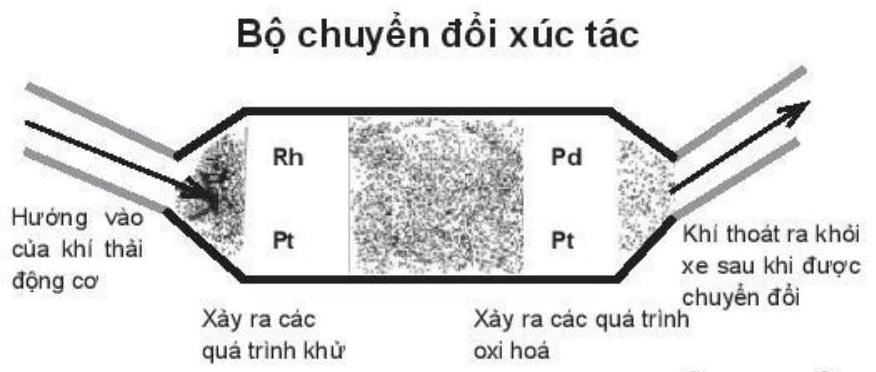
\includegraphics[max width=\textwidth, center]{2025_10_23_883c4b146e2332109fcdg-65(1)}

Thiết bị có sử dụng các kim loại platinum, rhodium và palladium để thúc đẩy quá trình nhường, nhận electron của chất trong khí thải, nó hoạt động theo cơ chế phản ứng oxi hoá - khử, chuyển đổi khoảng $98 \%$ khí thải độc hại thành khí ít độc hại hoặc không độc hại cho môi trường. Khí thải chứa các hydrocarbon bị oxi hoá thành carbon dioxide và nước, carbon monoxide thành carbon dioxide, các oxide của nitrogen bị khử thành nitrogen và oxygen giải phóng ra môi trường.\\
Thiết bị trên vận dụng yếu tố nào để tác động đến phản ứng?\\
16.14. Năm 1785, một vụ nổ xảy ra tại nhà kho nhà Giacomelli (Roma, Italia) làm nghề nghiền bột mi. Sau khi điều tra, nguyên nhân ban đầu dẫn đến vụ nổ là do bột mì khô. Sự cố xảy ra khi bột mì bay trong không khí, chạm tới nguồn lửa của chiếc đèn, đây là vụ nổ bụi đầu tiên trong lịch sử. Sau đó là các vụ nổ bụi trong hầm than, xưởng sản xuất sữa bột, dược phẩm, nhựa, kim loại, ... có tác nhân tương tự gồm: nguồn oxygen, nguồn nhiệt, bụi có thể cháy được, nồng độ bụi để đạt được vụ nổ và không gian đủ kín.\\
Thí nghiệm như hình bên cho thấy, bột mì không dễ cháy. Tại sao bột mì và một số loại bụi khác có thể gây ra nổ bụi? Để ngăn ngừa và hạn chế nổ bụi, có thể can thiệp vào những tác nhân nào?\\
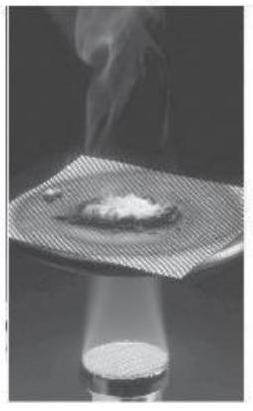
\includegraphics[max width=\textwidth, center]{2025_10_23_883c4b146e2332109fcdg-65}\\
16.15. Hệ thống phun nhiên liệu điện tử (Electronic Fuel Injection - EFI) được sử dụng trong động cơ ô tô, xe máy giúp tiết kiệm nhiên liệu, xe vận hành êm và giảm ô nhiểm môi trường. Hệ thống sử dụng bộ điều khiển điện tử để can thiệp vào bước phun nhiên liệu vào buồng đốt, nhiên liệu được phun giọt cực nhỏ (1); hệ thống điều chỉnh chính xác tỉ lệ nhiên liệu - không khí trước khi phun vào buồng đốt, một cách đồng đều, nhiên liệu được đốt cháy hoàn toàn (2). Khi phương tiện thay đổi vận tốc (tăng hoặc giảm), hệ thống sẽ nhanh chóng thay đổi lượng nhiên liệu - không khí phù hợp đề phun vào buồng đốt (3), nên\\
tiết kiệm nhiên liệu và giảm lượng khí thải gây ô nhiễm môi trường. Các ý (1), (2), (3) vận dụng yếu tố chính nào ảnh hưởng đến tốc độ phản ứng?\\
16.16. Aspirin (acetylsalicylic acid, $\mathrm{C}_{9} \mathrm{H}_{8} \mathrm{O}_{4}$ ) là thuốc hạ sốt, giảm đau, có tính kháng viêm, được sử dụng khá phổ biến trên thế giới, khoảng 25000 tấn mỗi năm. Khi uống aspirin, phản ứng thuỷ phân xảy ra như sau:\\
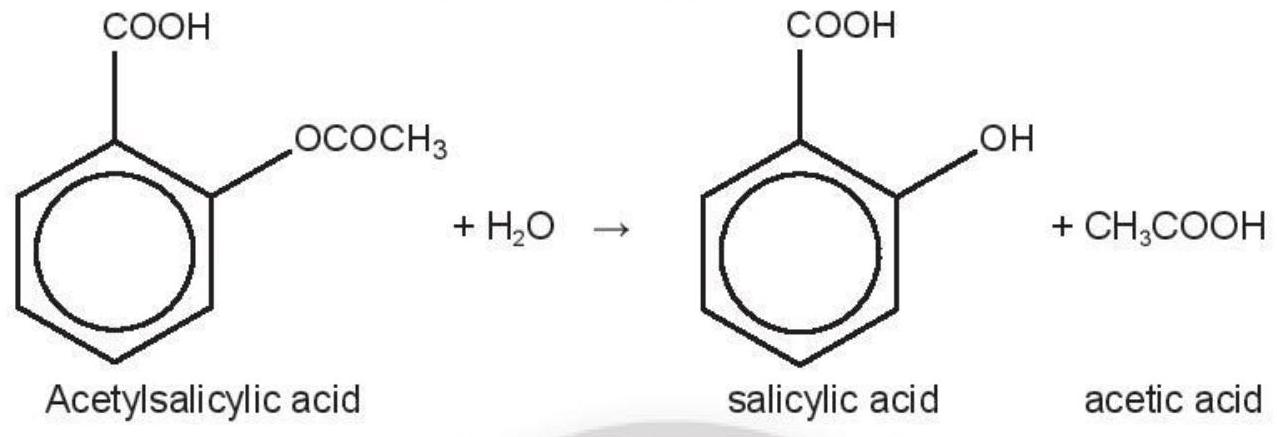
\includegraphics[max width=\textwidth, center]{2025_10_23_883c4b146e2332109fcdg-66}

Salicylic acid là thành phần chính có tác dụng hạ sốt, giảm đau và viêm nhiễm, nên có nhiều nghiên cứu tập trung vào phản ứng thuỷ phân này và các yếu tố ảnh hưởng đến tốc độ phản ứng. Dữ liệu về quá trình thuỷ phân của một mẫu aspirin trong nước (môi trường trung tính) ở $37^{\circ} \mathrm{C}$ ( ) thể hiện trong bảng:

\begin{center}
\begin{tabular}{|l|l|l|}
\hline
Thời gian (h) & Nồng độ aspirin (M) & Nồng độ salicylic acid (M) \\
\hline
0 & $5,55 \times 10^{-3}$ & 0 \\
\hline
2 & $5,51 \times 10^{-3}$ & $0,040 \times 10^{-3}$ \\
\hline
5 & $5,45 \times 10^{-3}$ & $0,10 \times 10^{-3}$ \\
\hline
10 & $5,35 \times 10^{-3}$ & $0,20 \times 10^{-3}$ \\
\hline
20 & $5,15 \times 10^{-3}$ & $0,40 \times 10^{-3}$ \\
\hline
30 & $4,96 \times 10^{-3}$ & $0,59 \times 10^{-3}$ \\
\hline
40 & $4,78 \times 10^{-3}$ & $0,77 \times 10^{-3}$ \\
\hline
50 & $4,61 \times 10^{-3}$ & $0,94 \times 10^{-3}$ \\
\hline
100 & $3,83 \times 10^{-3}$ & $1,72 \times 10^{-3}$ \\
\hline
200 & $2,64 \times 10^{-3}$ & $2,91 \times 10^{-3}$ \\
\hline
300 & $1,82 \times 10^{-3}$ & $3,73 \times 10^{-3}$ \\
\hline
\end{tabular}
\end{center}

(*) Ở điều kiện này, phản ứng xảy ra rất chậm, trong môi trường acid, như điều kiện trong dạ dày, phản ứng xảy ra nhanh hơn.\\
a) Tính tốc độ trung bình của phản ứng thuỷ phân aspirin sau thời gian 2,5 , $10, \ldots, 300$ giờ.\\
b) Nhận xét sự thay đổi tốc độ phản ứng theo thời gian. Giải thích.\\
c) Vẽ đồ thị biểu diễn sự biến thiên nồng độ chất tham gia và sản phẩm theo thời gian của phản ứng trên.\\
16.17. Hoạt động trong phòng thí nghiệm

\section*{Chuẩn bị}
Dưng cụ: Cân phân tích, cốc thuỷ tinh, đồng hồ bấm giây.\\
Hoá chất: $\mathrm{CaCO}_{3}$ dạng khối, dung dịch HCl 2 M .

\section*{Tiến hành}
Bước 1: Cân 5-7 viên đá vôi, ghi giá trị $m_{1}$.\\
Bước 2: Rót 100 ml dung dịch HCl vào cốc thuỷ tinh, cân khối lượng cốc, ghi giá trị $\mathrm{m}_{2}$.\\
Bước 3: Để yên cốc trên giá cân. Cho các viên đá vôi vào cốc dung dịch HCl . Ghi nhận tổng khối lượng hiển thị trên cân sau mối 30 giây, thực hiện trong 10 phút.

\section*{Yêu cầu}
\begin{enumerate}
  \item Vận dụng định luật bảo toàn khối lượng, tính khối lượng khí $\mathrm{CO}_{2}$ sau mỗi 30 giây.
  \item Tính tốc độ trung bình của phản ứng sau khoảng thời gian $1,2,3,4$ phút.
  \item Nhận xét tốc độ phản ứng thay đổi thế nào theo thời gian. Giải thích.
  \item Vẽ biểu đồ biểu diễn khối lượng $\mathrm{CO}_{2}$ trong các thời điểm khác nhau.
\end{enumerate}

\section*{ÔN TẬP CHƯONG 6}
OT6.1. Phản ứng $2 \mathrm{NO}(\mathrm{g})+\mathrm{O}_{2}(\mathrm{~g}) \rightarrow 2 \mathrm{NO}_{2}(\mathrm{~g})$ có biểu thức tốc độ tức thời: $v=k \times \mathrm{C}_{\mathrm{NO}}^{2} \times \mathrm{C}_{\mathrm{O}_{2}}$. Nếu nồng độ của NO giảm 2 lần, giữ nguyên nồng độ oxygen, thì tốc độ sẽ\\
A. giảm 2 lần.\\
B. giảm 4 lần.\\
C. giảm 3 lần.\\
D. giữ nguyên.

OT6.2. Nếu mỗi đồ thị có các chất phản ứng cùng nồng độ và trục thời gian thì tốc độ của chất phản ứng nào xảy ra nhanh nhất?

\begin{figure}[h]
\begin{center}
\captionsetup{labelformat=empty}
\caption{A.}
  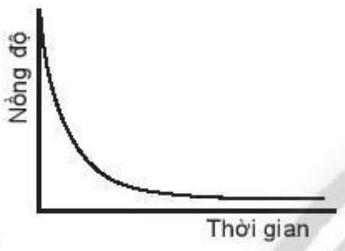
\includegraphics[width=\textwidth]{2025_10_23_883c4b146e2332109fcdg-68(2)}
\end{center}
\end{figure}

\begin{figure}[h]
\begin{center}
\captionsetup{labelformat=empty}
\caption{B.}
  \includegraphics[width=\textwidth]{2025_10_23_883c4b146e2332109fcdg-68(3)}
\end{center}
\end{figure}

\begin{figure}[h]
\begin{center}
\captionsetup{labelformat=empty}
\caption{C.}
  \includegraphics[width=\textwidth]{2025_10_23_883c4b146e2332109fcdg-68}
\end{center}
\end{figure}

\begin{figure}[h]
\begin{center}
\captionsetup{labelformat=empty}
\caption{D.}
  \includegraphics[width=\textwidth]{2025_10_23_883c4b146e2332109fcdg-68(1)}
\end{center}
\end{figure}

OT6.3. Thanh phát sáng là một sản phẩm quen thuộc được dùng giải trí. Đặt 2 thanh phát quang hoá học vào 2 cốc nước nóng (trái) và lạnh (phải) như hình bên, yếu tố ảnh hưởng đến độ phát sáng của 2 thanh là\\
A. nồng độ.\\
B. chất xúc tác.\\
C. bề mặt tiếp xúc.\\
D. nhiệt độ.\\
\includegraphics[max width=\textwidth, center]{2025_10_23_883c4b146e2332109fcdg-68(4)}

OT6.4. Trong hầu hết các phản ứng hoá học, tốc độ phản ứng tăng khi nhiệt độ tăng. Muốn pha một cốc trà đá có đường, bằng cách thêm đá viên và đường vào cốc trà nóng, thứ tự nào sẽ được cho vào trước?

OT6.5. Cho phương trình hoá học của phản ứng:

$$
2 \mathrm{CO}(g)+\mathrm{O}_{2}(g) \rightarrow 2 \mathrm{CO}_{2}(g)
$$

Với biểu thức tốc độ tức thời là: $v=k \times \mathrm{C}_{\mathrm{CO}}^{2} \times \mathrm{C}_{\mathrm{O}_{2}}$, khi nồng độ mol của CO là 1 M và $\mathrm{O}_{2}$ là 1 M , tính giá trị $v$ và nêu ý nghĩa của $k$.

OT6.6. Từ thí nghiệm ảnh hưởng của bề mặt tiếp xúc đến tốc độ phản ứng trong SGK trang 101, 102, nếu ở bình (2), sau thời gian 60 giây, thể tích khí $\mathrm{CO}_{2}$ thu được là 30 mL . Tính tốc độ trung bình ( $\mathrm{mL} / \mathrm{s}$ ) của phản ứng trong 60 giây.

OT6.7. Trong phản ứng: $\mathrm{A} \rightarrow$ sản phẩm\\
Tại thời điểm $t=0$, nồng độ chất $A$ là $0,1563 \mathrm{M}$, sau 1 phút, nồng độ chất $A$ là $0,1496 \mathrm{M}$ và sau 2 phút, nồng độ chất A là $0,1431 \mathrm{M}$.\\
a) Tính tốc độ trung bình của phản ứng trong phút thứ nhất và trong phút thứ 2 .\\
b) Nhận xét tốc độ phản ứng trong phút thứ nhất và phút thứ 2. Giải thích.

OT6.8. Xét phản ứng phân huỷ $\mathrm{N}_{2} \mathrm{O}_{5}$ theo phương trình hoá học:\\
$2 \mathrm{~N}_{2} \mathrm{O}_{5}(g) \rightarrow 4 \mathrm{NO}_{2}(g)+\mathrm{O}_{2}(g)$, xảy ra ở $56^{\circ} \mathrm{C}$ cho kết quả theo bảng:

\begin{center}
\begin{tabular}{|c|c|c|c|}
\hline
Thòi gian (s) & $\mathbf{N}_{2} \mathbf{O}_{5} \mathbf{( M )}$ & $\mathbf{N O}_{2} \mathbf{( M )}$ & $\mathbf{O}_{2} \mathbf{( M )}$ \\
\hline
240 & 0,0388 & 0,0315 & 0,0079 \\
\hline
600 & 0,0196 & 0,0699 & 0,0175 \\
\hline
\end{tabular}
\end{center}

Tính tốc độ trung bình của phản ứng trong khoảng thời gian trên.\\
OT6.9. Sự phân huỷ $\mathrm{H}_{2} \mathrm{O}_{2}$ theo phương trình hoá học: $2 \mathrm{H}_{2} \mathrm{O}_{2}(a q) \rightarrow 2 \mathrm{H}_{2} \mathrm{O}(l)+\mathrm{O}_{2}(g)$, được nghiên cứu và cho kết quả tại một nhiệt độ cụ thể như sau:

\begin{center}
\begin{tabular}{|l|l|}
\hline
Thời gian (s) & $\mathrm{H}_{2} \mathrm{O}_{2}(\mathrm{~mol} / \mathrm{L})$ \\
\hline
0 & 1,000 \\
\hline
120 & 0,910 \\
\hline
300 & 0,780 \\
\hline
600 & 0,590 \\
\hline
1200 & 0,370 \\
\hline
1800 & 0,220 \\
\hline
2400 & 0,130 \\
\hline
3000 & 0,082 \\
\hline
3600 & 0,050 \\
\hline
\end{tabular}
\end{center}

a) Tính tốc độ trung bình của phản ứng phân huỷ $\mathrm{H}_{2} \mathrm{O}_{2}$ theo thời gian.\\
b) Tốc độ phản ứng thay đổi thế nào theo thời gian? Giải thích sự thay đổi đó.

\section*{Chuong 7. NGUYÊN TÓ NHÓM VIIA - HALOGEN}
\section*{TÍNH CHẤT VẬT LÍ VÀ HOÁ HỌC CÁC ĐƠN CHẤT NHÓM VIIA}
17.1. Trong bảng tuần hoàn các nguyên tố hoá học, halogen thuộc nhóm\\
A. IA.\\
B. IIA.\\
C. VIIA.\\
D. VIIIA.\\
17.2. Halogen tồn tại thể lỏng ở điều kiện thường là\\
A. fluorine.\\
B. bromine.\\
C. Iodine.\\
D. chlorine.\\
17.3. Đơn chất halogen ở thể khí, màu vàng lục là\\
A. chlorine.\\
B. Iodine.\\
C. bromine.\\
D. fluorine.\\
17.4. Nguyên tố có tính oxi hoá yếu nhất thuộc nhóm VIIA là\\
A. chlorine.\\
B. lodine.\\
C. bromine.\\
D. fluorine.\\
17.5. Cấu hình electron nguyên tử thuộc nguyên tố halogen là\\
A. $n s^{2} n p^{2}$.\\
B. $n s^{2} n p^{3}$.\\
C. $n s^{2} n p^{5}$.\\
D. $\mathrm{ns}^{2} \mathrm{np}^{6}$.\\
17.6. Ứng dụng nào sau đây không phải của $\mathrm{Cl}_{2}$ ?\\
A. Xử lí nước bể bơi.\\
B. Sát trùng vết thương trong y tế.\\
C. Sản xuất nhựa PVC.\\
D. Sản xuất bột tầy trắng.\\
17.7. Halogen nào được dùng trong sản xuất nhựa Teflon?\\
A. Chlorine.\\
B. Iodine.\\
C. Fluorine.\\
D. Bromine.\\
17.8. Nguyên tố halogen được dùng trong sản xuất nhựa PVC là\\
A. chlorine.\\
B. bromine.\\
C. phosphorus.\\
D. carbon.\\
17.9. Halogen được điều chế bằng cách điện phân có màn ngăn dung dịch muối ăn là\\
A. fluorine.\\
B. chlorine.\\
C. bromine.\\
D. Iodine.\\
17.10. Nguyên tố halogen dùng làm gia vị, cần thiết cho tuyến giáp và phòng ngừa khuyết tật trí tuệ là\\
A. chlorine.\\
B. iodine.\\
C. bromine.\\
D. fluorine.\\
17.11. Halogen nào tạo liên kết ion bền nhất với sodium?\\
A. Chlorine.\\
B. Bromine.\\
C. lodine.\\
D. Fluorine.\\
17.12. Liên kết trong phân tử đơn chất halogen là\\
A. liên kết van der Waals.\\
B. liên kết cộng hoá trị.\\
C. liên kết ion.\\
D. liên kết cho nhận.\\
17.13. Theo chiều từ $\mathrm{F} \rightarrow \mathrm{Cl} \rightarrow \mathrm{Br} \rightarrow \mathrm{I}$, bán kính của nguyên tử\\
A. tăng dần.\\
B. giảm dần.\\
C. không thay đổi.\\
D. không có quy luật.\\
17.14. Đặc điểm của halogen là\\
A. nguyên tử chỉ nhận thêm 1 electron trong các phản ứng hoá học.\\
B. tạo liên kết cộng hoá trị với nguyên tử hydrogen.\\
C. nguyên tử có số oxi hoá -1 trong tất cả hợp chất.\\
D. nguyên tử có 5 electron hoá trị.\\
17.15. Phát biểu nào sau đây là không đúng?\\
A. Trong tự nhiên, không tồn tại đơn chất halogen.\\
B. Tính oxi hoá của đơn chất halogen giảm dần từ $F_{2}$ đến $I_{2}$.\\
C. Khí chlorine ẩm và nước chlorine đều có tính tẩy màu.\\
D. Fluorine có tính oxi hoá mạnh hơn chlorine, oxi hoá $\mathrm{Cl}^{-}$trong dung dịch NaCl thành $\mathrm{Cl}_{2}$.\\
17.16. Giá trị độ âm điện của halogen và hydrogen trong bảng sau:

\begin{center}
\begin{tabular}{|c|c|c|c|c|c|}
\hline
Nguyên tố & H & F & Cl & Br & I \\
\hline
Giá trị độ âm điện & 2,20 & 3,98 & 3,16 & 2,96 & 2,66 \\
\hline
\end{tabular}
\end{center}

Dựa vào giá trị độ âm điện, sắp xếp theo thứ tự giảm dần khả năng liên kết của halogen với hydrogen. So sánh độ phân cực của các phân tử hydrogen halide.\\
17.17. Cho phương trình hoá học của 2 phản ứng như sau:

$$
\begin{aligned}
\mathrm{Cl}_{2}+2 \mathrm{NaBr} & \rightarrow 2 \mathrm{NaCl}+\mathrm{Br}_{2} \\
\mathrm{Br}_{2}+2 \mathrm{Nal} & \rightarrow 2 \mathrm{NaBr}+\mathrm{I}_{2}
\end{aligned}
$$

Phương trình chứng minh tính chất nào của halogen?\\
17.18. Hoàn thành phương trình hoá học của các phản ứng chứng minh tính chất halogen:\\
a) $\mathrm{Br}_{2}+\mathrm{K} \rightarrow$\\
b) $\mathrm{F}_{2}+\mathrm{H}_{2} \mathrm{O} \rightarrow$\\
c) $\mathrm{Cl}_{2}+\mathrm{Ca}(\mathrm{OH})_{2} \rightarrow$\\
d) $\mathrm{Cl}_{2}+\mathrm{NaI} \rightarrow$

Nhận xét vai trò của halogen trong các phản ứng trên.\\
17.19. Muối NaCl có lẫn một ít Nal. Nhận biết sự có mặt của muối Nal có trong hỗn hợp.\\
17.20. Trong hợp chất, số oxi hoá của halogen (trừ F ) thường là $-1,+1,+3,+5,+7$.

Tại sao các số oxi hoá chẵn không đặc trưng đối với halogen trong hợp chất?\\
17.21. Tại sao trong hợp chất của halogen, nguyên tố fluorine chỉ thể hiện số oxi hoá -1 , còn các nguyên tố chlorine, bromine, iodine là $-1,+1,+3,+5,+7$ ?\\
17.22. Tại sao đơn chất halogen ít tan trong nước, tan nhiều trong dung môi hữu cơ không phân cực như hexane $\left(\mathrm{C}_{6} \mathrm{H}_{14}\right)$, carbon tetrachloride $\left(\mathrm{CCl}_{4}\right)$ ?\\
17.23. Tại sao chỉ có tên gọi nước chlorine, bromine, iodine nhưng không có nước fluorine?\\
17.24. Một học sinh thực hiện thí nghiệm và cho kết quả như sau:

Bước 1: Lấy 2 mL dung dịch NaBr vào ống nghiệm, dung dịch không màu.\\
Bước 2: Lấy tiếp 1 mL hexane vao ống nghiệm, lắc mạnh để quan sát khả năng hoà tan của 2 chất lỏng. Nhận thấy 2 chất lỏng không tan vào nhau và phân tách lớp.\\
Bước 3: Thêm 1 mL nước $\mathrm{Cl}_{2}$ vào ống nghiệm, lắc đều rồi để yên. Quan sát thấy lớp chất lỏng phía trên có màu da cam.\\
Viết phương trình hoá học của phản ứng. Thí nghiệm trên chứng minh tính chất vật lí và hoá học nào của halogen tương ứng?\\
17.25. Xác nhận đúng, sai cho các phát biểu trong bảng sau:

\begin{center}
\begin{tabular}{|l|l|l|l|}
\hline
\multirow{2}{*}{STT} & \multirow{2}{*}{Phát biểu} & \multicolumn{2}{|r|}{Xác nhận} \\
\hline
 &  & Đúng & Sai \\
\hline
1 & Halogen vừa có tính oxi hoá, vừa có tính khử &  &  \\
\hline
2 & Nước chlorine và Javel đều có tính tầy màu &  &  \\
\hline
3 & Halogen tồn tại cả đơn chất và hợp chất trong tự nhiên &  &  \\
\hline
4 & $\mathrm{Cl}_{2}$ có tính oxi hoá mạnh hơn $\mathrm{Br}_{2}$ &  &  \\
\hline
5 & $\mathrm{Cl}_{2}$ khử được $\mathrm{I}^{-}$trong dung dịch NaI thành $\mathrm{I}_{2}$ &  &  \\
\hline
6 & Nhỏ nước iodine vào mặt cắt củ khoai, xuất hiện màu xanh đen &  &  \\
\hline
7 & Hợp chất của fluorine làm thuốc chống sâu răng, chất dẻo Teflon &  &  \\
\hline
\end{tabular}
\end{center}

17.26. Các hợp chất hypochlorite hay Chlorine ( $\mathrm{NaClO}, \mathrm{Ca}(\mathrm{ClO})_{2}$ ) là các hoá chất có tính oxi hoá rất mạnh, có khả năng sát trùng, sát khuẩn, làm sạch nguồn nước (Chlorine được nhắc đến là tên thương mại, không phải đơn chất $\mathrm{Cl}_{2}$ ). Chlorine ở nồng độ xác định có khả năng tiêu diệt một số mầm bệnh như:

\begin{center}
\begin{tabular}{|l|l|}
\hline
Mầm bệnh & Thời gian tiêu diệt \\
\hline
E. coli O157: H7 (gây tiêu chảy ra máu, suy thận) & < 1 phút \\
\hline
Hepatilis A virus (gây bệnh viêm gan siêu vi A) & 16 phút \\
\hline
Ki sinh trùng Giardia (gây tiêu chảy, đau bụng và sụt cân) & 45 phút \\
\hline
\end{tabular}
\end{center}

Chlorine cần dùng là tổng lượng chlorine cần thiết để tiêu diệt mầm bệnh và oxi hoá các chất khử trong nước như iron, manganese, hydrogen sulfide và lượng chlorine tự do còn lại sau khoảng thời gian nhất định. Một nhà máy xử lí nước muốn làm sạch 1 lít nước thì lượng chlorine cần dùng trong 1 ngày là 11 mg để duy trì lượng chlorine tự do từ 0,1 đến $0,2 \mathrm{mg} / \mathrm{L}$ tại vòi sử dụng. Một ngày, nhà máy phải cung cấp $3000 \mathrm{~m}^{3}$ nước xử lí, thì lượng chlorine cần dùng là bao nhiêu?\\
17.27. Việt Nam là nước xuất khẩu thuỷ sản thứ 3 trên thế giới, sau Na Uy và Trung Quốc (Theo Bộ Nông nghiệp và Phát triển nông thôn Việt Nam, tháng 12/2021), xuất khẩu tới hơn 170 nước trên thế giới, trong đó có thị trường lớn như Mỹ và Châu Âu, được xem là thị trường khó tính, nên tiêu chuẩn chất lượng được kiểm soát chặt chẽ trước khi nhập nguyên liệu và sau khi thành phẩm, đóng gói. Trong danh mục tiêu chuẩn chất lượng sản phẩm có chỉ tiêu về dư lượng chlorine không vượt quá $1 \mathrm{mg} / \mathrm{L}$ (chlorine sử dụng trong quá trình sơ chế nguyên liệu để diệt vi sinh vật).\\
Phương pháp chuẩn độ iodine-thiosulfate được dùng để xác định dư lượng chlorine trong thực phẩm theo phương trình: $\quad \mathrm{Cl}_{2}+2 \mathrm{KI} \rightarrow 2 \mathrm{KCl}+\mathrm{I}_{2}$\\
$\mathrm{I}_{2}$ được nhận biết bằng hồ tinh bột, $\mathrm{I}_{2}$ bị khử bởi dung dịch chuẩn sodium thiosulfate theo phương trình: $\mathrm{I}_{2}+2 \mathrm{Na}_{2} \mathrm{~S}_{2} \mathrm{O}_{3} \rightarrow 2 \mathrm{NaI}+\mathrm{Na}_{2} \mathrm{~S}_{4} \mathrm{O}_{6}$.\\
Dựa vào thể tích dung dịch $\mathrm{Na}_{2} \mathrm{~S}_{2} \mathrm{O}_{3}$ phản ứng, tính được dư lượng chlorine trong dung dịch mẫu.\\
Tiến hành chuẩn độ 100 mL dung dịch mẫu bằng dung dịch $\mathrm{Na}_{2} \mathrm{~S}_{2} \mathrm{O}_{3} 0,01 \mathrm{M}$, thể tích $\mathrm{Na}_{2} \mathrm{~S}_{2} \mathrm{O}_{3}$ dùng hết $0,28 \mathrm{~mL}$ (dụng cụ chứa dung dịch chuẩn $\mathrm{Na}_{2} \mathrm{~S}_{2} \mathrm{O}_{3}$ là loại microburet 1 mL , vạch chia $0,01 \mathrm{~mL}$ ). Mẫu sản phẩm trên đủ tiêu chuẩn về dư lượng chlorine cho phép để xuất khẩu không? Giải thích.

\section*{18}
\section*{HYDROGEN HALIDE VÀ MỘT SỐ PHẢN ÚNG CỦA ION HALIDE}
18.1. Hydrogen halide có nhiệt độ sôi cao nhất là\\
A. HI .\\
B. HCl .\\
C. HBr .\\
D. HF .\\
18.2. Phân tử có tương tác van der Waals lớn nhất là\\
A. HCl .\\
B. HI .\\
C. HBr .\\
D. HF .\\
18.3. Hydrohalic acid có tính acid mạnh nhất là\\
A. HF .\\
B. HBr .\\
C. HI.\\
D. HCl .\\
18.4. Hydrohalic acid có tính ăn mòn thuỷ tinh là\\
A. HBr .\\
B. HI .\\
C. HCl .\\
D. HF .\\
18.5. Liên kết hydrogen của phân tử nào được biểu diễn đúng?\\
A. $\ldots \mathrm{H}-\mathrm{I} \ldots \mathrm{H}-\mathrm{I} \ldots \mathrm{H}-\mathrm{I} \ldots$\\
B. $\ldots \mathrm{H}-\mathrm{Cl} \ldots \mathrm{H}-\mathrm{Cl} \ldots \mathrm{H}-\mathrm{Cl} \ldots$\\
C. $\ldots \mathrm{H}-\mathrm{Br} \ldots \mathrm{H}-\mathrm{Br} \ldots \mathrm{H}-\mathrm{Br} \ldots$\\
D. $\ldots \mathrm{H}-\mathrm{F} \ldots \mathrm{H}-\mathrm{F} \ldots \mathrm{H}-\mathrm{F}$\\
18.6. Ion halide được sắp xếp theo chiều giảm dần tính khử:\\
A. $\mathrm{F}^{-}, \mathrm{Cl}^{-}, \mathrm{Br}^{-}, \mathrm{I}^{-}$.\\
B. $\mathrm{I}^{-}, \mathrm{Br}^{-}, \mathrm{Cl}^{-}, \mathrm{F}^{-}$.\\
C. $\mathrm{F}^{-}, \mathrm{Br}^{-}, \mathrm{Cl}^{-}, \mathrm{I}^{-}$.\\
D. $\mathrm{I}^{-}, \mathrm{Br}^{-}, \mathrm{F}^{-}, \mathrm{Cl}^{-}$.\\
18.7. Hydrogen halide có nhiều liên kết hydrogen nhất với nước là\\
A. HF .\\
B. HCl .\\
C. HBr .\\
D. HI.\\
18.8. Chất hay ion nào có tính khử mạnh nhất?\\
A. $\mathrm{Cl}_{2}$.\\
B. $\mathrm{Cl}^{-}$.\\
C. $I_{2}$.\\
D. $I^{-}$.\\
18.9. Dung dịch dùng để nhận biết các ion halide là\\
A. Quỳ tím.\\
B. $\mathrm{AgNO}_{3}$.\\
C. NaOH .\\
D. HCl .\\
18.10. Rót 3 mL dung dịch HBr 1 M vào 2 mL dung dịch NaOH 1 M , cho quỳ tím vào dung dịch sau phản ứng, mẩu quỳ tím sẽ\\
A. hoá màu đỏ.\\
B. hoá màu xanh.\\
C. mất màu tím.\\
D. không đổi màu.\\
18.11. Trong phòng thí nghiệm, chlorine được điều chế bằng cách oxi hoá hợp chất\\
A. NaCl .\\
B. HCl .\\
C. $\mathrm{KMnO}_{4}$.\\
D. $\mathrm{KClO}_{3}$.\\
18.12. Cách thu khí hydrogen halide trong phòng thí nghiệm phù hợp là:

\begin{figure}[h]
\begin{center}
  \includegraphics[width=\textwidth]{2025_10_23_883c4b146e2332109fcdg-75(1)}
\captionsetup{labelformat=empty}
\caption{Hình 1}
\end{center}
\end{figure}

\begin{figure}[h]
\begin{center}
  \includegraphics[width=\textwidth]{2025_10_23_883c4b146e2332109fcdg-75(2)}
\captionsetup{labelformat=empty}
\caption{Hinh 2}
\end{center}
\end{figure}

\begin{figure}[h]
\begin{center}
  \includegraphics[width=\textwidth]{2025_10_23_883c4b146e2332109fcdg-75}
\captionsetup{labelformat=empty}
\caption{Hinh 3}
\end{center}
\end{figure}

A. Hinh 1.\\
B. Hinh 2.\\
C. Hinh 3.\\
D. Hình 1 và 2.\\
18.13. Chọn phát biểu không đúng:\\
A. Các hydrogen halide tan tốt trong nước tạo dung dịch acid.\\
B. Ion $\mathrm{F}^{-}$và $\mathrm{Cl}^{-}$không bị oxi hoá bởi dung dịch $\mathrm{H}_{2} \mathrm{SO}_{4}$ đặc.\\
C. Các hydrogen halide làm quỳ tím hoá đỏ.\\
D. Tính acid của các hydrohalic acid tăng dần từ HF đến HI .\\
18.14. Hydrogen chloride được điều chế bằng cách cho tinh thể sodium chloride tác dụng với sulfuric acid đặc. Tuy nhiên, không thể dùng phương pháp này để điều chế hydrogen bromide. Nêu nguyên nhân và đề nghị phương pháp hoá học điều chế hydrogen bromide.\\
18.15. Dung dịch HBr và HI đậm đặc không màu, thường được đựng trong lọ thuỷ tinh sẩm màu, sau một thời gian sử dụng, dưới ảnh hưởng của không khí, dung dịch HBr có màu vàng cam, dung dịch HI có màu vàng đậm. Giải thích sự thay đồi màu sắc của 2 dung dịch acid trên.\\
18.16. Cho bảng thông tin sau:

\begin{center}
\begin{tabular}{|l|l|l|l|l|}
\hline
Đặc điểm & HF & $\mathbf{H C l}$ & HBr & HI \\
\hline
Năng lượng liên kết ( $\mathrm{kJ} / \mathrm{mol}$ ) & 565 & 427 & 363 & 295 \\
\hline
Độ dài liên kết ( $\AA$ ) & 0,92 & 1,27 & 1,41 & 1,61 \\
\hline
\begin{tabular}{l}
Hằng số điện li acid $\left(\mathrm{K}_{\mathrm{a}}\right)^{(*)}$ \\
(*) Đại lượng đo độ mạnh của một acid trong dung dịch \\
\end{tabular} & $7 \times 10^{-4}$ & $1 \times 10^{7}$ & $1 \times 10^{9}$ & $1 \times 10^{10}$ \\
\hline
\end{tabular}
\end{center}

a) Sắp xếp theo thứ tự giảm dần tính acid của các hydrohalic acid.\\
b) Dựa vào bảng thông tin, giải thích thứ tự tính acid của các hydrohalic acid.\\
18.17. Đặt cốc thuỷ tinh lên cân, chỉnh cân về số 0 , rót vào cốc dung dịch HCl 1 M đến khối lượng 100 g . Thêm tiếp 1 lượng bột magnesium vào cốc, khi không còn khí thoát ra, cân thể hiện giá trị $105,5 \mathrm{~g}$.\\
a) Khối lượng magnesium thêm vào là bao nhiêu?\\
b) Tính khối lượng muối và thể tích khí hydrogen (đkc) được tạo ra.\\
18.18. Trong chế độ dinh đưỡng của trẻ sơ sinh và trẻ nhỏ rất chú trọng thành phần sodium chloride $(\mathrm{NaCl})$ trong thực phẩm. Theo khuyến cáo của Tổ chức Y tế thế giới (WHO), lượng muối cần thiết trong 1 ngày đối với trẻ sơ sinh là $0,3 \mathrm{~g}$, với trẻ dưới 1 tuổi là $1,5 \mathrm{~g}$, dưới 2 tuổi là $2,3 \mathrm{~g}$. Nếu trẻ ăn thừa muối sẽ ảnh hưởng đến hệ bài tiết, thận, tăng nguy cơ còi xương, ... Trẻ ăn thừa muối có xu hướng ăn mặn hơn bình thường và là một trong những nguyên nhân làm tăng huyết áp, suy thận, ung thư khi trưởng thành. Ở từng nhóm tuổi trên, tính lượng ion chloride trong NaCl cho cơ thể mỗi ngày.\\
18.19. "Muối i-ốt" có thành phần chính là sodium chloride $(\mathrm{NaCl})$ có bổ sung một lượng nhỏ potassium iodide (KI) nhằm bổ sung nguyên tố vi lượng iodine cho cơ thể, nhằm ngăn bệnh bứu cổ, phòng ngừa khuyết tật trí tuệ và phát triển, ... Trong 100 g muối i-ốt có chứa hàm lượng ion iodide dao động từ $2200 \mu \mathrm{~g}$ $2500 \mu \mathrm{~g}$; Iượng iodide cần thiết cho một thiếu niên hay người trưởng thành từ $66 \mu \mathrm{~g}-110 \mu \mathrm{~g} / \mathrm{ng}$ ày. Trung bình, một thiếu niên hay trưởng thành cần bao nhiêu g muối i-ốt trong một ngày?\\
18.20. Rong biển, còn gọi là tảo bẹ, loài sinh vật sống dưới biển, được xem là nguồn thực phẩm có giá trị dinh dưỡng cao cho con người. Rong biển khô cung cấp đường, chất xơ, đạm, vitamin A , vitamin B2 và muối khoáng. Trong đó, thành phần được quan tâm hơn cả là nguyên tố vi lượng iodine. Trung bình, trong 100 gam tảo bẹ khô có chứa khoảng $1000 \mu \mathrm{~g}$ iodine. Để sản xuất 1 tấn iodine thì cần bao nhiêu tấn tảo bẹ khô?\\
18.21. Ninh Thuận là tỉnh có 3 trong số 7 đồng muối lớn của cả nước là Cà Ná, Tri Hải và Đầm Vua, sản lượng muối của Ninh Thuận chiếm khoảng $50 \%$ sản lượng muối cả nước. Nghề làm muối truyền thống có quy trình: cải tạo ô ruộng muối, dẫn nước biển vào, phơi nắng để nước biển bốc hơi và thu hoạch muối. Sản lượng muối hằng năm đạt hơn 426500 tấn (giai đoạn 2021 - 2025), tăng trưởng 650000 tấn (đến năm 2030) đảm bảo cho yêu cầu phát triển công nghiệp, tạo việc làm cho lực lượng lao động địa phương (theo Thông tấn xã Việt Nam).\\
Nước biển từ biển và đại dương có độ mặn khoảng 3,5\% (độ mặn không đồng nhất trên toàn cầu, phần lớn từ $3,1-3,8 \%$ ), với khối lượng riêng $1,02-1,03 \mathrm{~g} / \mathrm{mL}$, nghĩa là mỗi lít nước biển có khoảng 36 g muối. Độ mặn được tính bằng tổng lượng (đơn vị gam) hoà tan của 11 ion chính (chiếm $99,99 \%$ ) là: $\mathrm{Na}^{+}, \mathrm{Ca}^{2+}, \mathrm{Mg}^{2+}, \mathrm{Fe}^{3+}, \mathrm{NH}_{4}{ }^{+}, \mathrm{Cl}^{-}, \mathrm{SO}_{4}{ }^{2-}, \mathrm{HCO}_{3}{ }^{-}, \mathrm{CO}_{3}{ }^{2-}, \mathrm{NO}_{2}{ }^{-}, \mathrm{NO}_{3}{ }^{-}$ có trong 1 kg nước biển, trong đó ion $\mathrm{Cl}^{-}(55,04 \%), \mathrm{Na}^{+}(30,61 \%), \mathrm{SO}_{4}{ }^{2-} (7,68 \%)$ và $\mathrm{Mg}^{2+}(3,69 \%)$.\\
a) Để khai thác được sản lượng 426500 tấn/ năm như hiện tại và 650 000/ năm (đến năm 2030) thì thể tích nước biển cần dẫn vào ruộng muối là bao nhiêu? (Tính toán nhằm cung cấp số liệu để tính diện tích ruộng muối, từ đó xây dựng quy trình sản xuất để đạt năng suất cao hơn, ...)\\
b) Tính khối lượng ion chloride được khai thác từ nước biển hàng năm.

\section*{ÔN TẬP CHƯONG 7}
OT7.1. Cấu hình electron nào của nguyên tử halogen?\\
A. $1 s^{2} 2 s^{2} 2 p^{6}$.\\
B. $1 s^{2} 2 s^{2} 2 p^{6} 3 s^{2}$.\\
C. $1 s^{2} 2 s^{2} 2 p^{6} 3 s^{2} 3 p^{5}$.\\
D. $1 s^{2} 2 s^{2} 2 p^{6} 3 s^{2} 3 p^{6} 4 s^{2} 3 d^{7}$.

OT7.2. Dung dịch $\mathrm{AgNO}_{3}$ không tác dụng với dung dịch.\\
A. NaI.\\
B. NaF .\\
C. NaCl .\\
D. NaBr

OT7.3. Phương trình hoá học nào viết sai?\\
A. $\mathrm{Br}_{2}+\mathrm{Cu} \rightarrow \mathrm{CuBr}_{2}$\\
B. $2 \mathrm{HCl}+\mathrm{Na}_{2} \mathrm{CO}_{3} \rightarrow 2 \mathrm{NaCl}+\mathrm{H}_{2} \mathrm{O}+\mathrm{CO}_{2}$\\
C. $\mathrm{NaBr}+\mathrm{AgNO}_{3} \rightarrow \mathrm{AgBr}+\mathrm{NaNO}_{3}$\\
D. $\mathrm{Cl}_{2}+\mathrm{Fe} \rightarrow \mathrm{FeCl}_{2}$

OT7.4. Nước chlorine có tính tẩy màu là do:\\
A. HCl có tính acid mạnh.\\
B. $\mathrm{Cl}_{2}$ vừa có tính khử vừa có tính oxi hoá.\\
C. HClO có tính oxi hoá mạnh.\\
D. $\mathrm{Cl}_{2}$ có tính oxi hoá mạnh.

OT7.5. Halogen không có tính khử là\\
A. fluorine.\\
B. bromine.\\
C. iodine.\\
D. chlorine.

OT7.6. Phương trình hoá học của 2 phản ứng như sau:

$$
\begin{aligned}
\mathrm{Cl}_{2}+2 \mathrm{NaBr} & \rightarrow 2 \mathrm{NaCl}+\mathrm{Br}_{2} \\
\mathrm{Br}_{2}+2 \mathrm{NaI} & \rightarrow 2 \mathrm{NaBr}+\mathrm{I}_{2}
\end{aligned}
$$

So sánh tính khử của các ion halide qua 2 phản ứng. Giải thích.\\
OT7.7. Ghi hiện tượng vào các ô trống trong bảng và viết phương trình hoá học của phản ứng (nếu có).

\begin{center}
\begin{tabular}{|c|c|c|c|c|c|}
\hline
Mẫu chất & \begin{tabular}{c}
Dung dịch \\
potassium \\
fluoride \\
\end{tabular} & \begin{tabular}{c}
Dung dịch \\
potassium \\
chloride \\
\end{tabular} & \begin{tabular}{c}
Dung dịch \\
potassium \\
bromide \\
\end{tabular} & \begin{tabular}{c}
Dung dịch \\
potassium \\
iodide \\
\end{tabular} & \begin{tabular}{c}
Cánh hoa \\
hồng \\
\end{tabular} \\
\hline
Nước chlorine &  &  &  &  &  \\
\hline
\end{tabular}
\end{center}

OT7.8. Chlorine tạo được các acid có oxygen trong thành phần phân tử. Tên và công thức của các acid có oxygen của chlorine theo bảng:

\begin{center}
\begin{tabular}{|l|l|l|l|}
\hline
HClO & Hypochlorous acid & $\mathrm{ClO}^{-}$ & Hypochlorite \\
\hline
$\mathrm{HClO}_{2}$ & Chlorous acid & $\mathrm{ClO}_{2}^{-}$ & Chlorite \\
\hline
$\mathrm{HClO}_{3}$ & Chloric acid & $\mathrm{ClO}_{3}^{-}$ & Chlorate \\
\hline
$\mathrm{HClO}_{4}$ & Perchloric acid & $\mathrm{ClO}_{4}^{-}$ & Perchlorate \\
\hline
\end{tabular}
\end{center}

Acid có hậu tố -ous thì tạo muối có hậu tố -ite; acid có hậu tố -ic tạo muối có hậu tố -ate; acid có mức oxi hoá của nguyên tố trung tâm thấp nhất có tiền tố hypo-; acid có mức oxi hoá của nguyên tố trung tâm cao nhất có tiền tố per-. Áp dụng quy tắc trên, đọc tên các chất sau: $\mathrm{HBrO} ; \mathrm{HBrO}_{2} ; \mathrm{HBrO}_{3}$; $\mathrm{HBrO}_{4} ; \mathrm{NaBrO} ; \mathrm{KBrO}_{2} ; \mathrm{KBrO}_{3}$ và $\mathrm{KBrO}_{4}$.

OT7.9. Nghiền mịn 10 g một mẫu đá vôi trong tự nhiên, hoà tan trong lượng dư dung dịch HCl thu được 4 g khí carbonic. Tính hàm lượng calcium carbonate trong mẫu đá vôi.


\end{document}